\documentclass[10pt]{article}
\usepackage[utf8]{inputenc}
\usepackage{titlesec}

\title{\Huge \textbf{Eletromagnetismo 1 - Relatório do Projeto}}
\author{
Aluno: Victor Miguel de Morais Costa (vmmc2) \\
Professor: Odilon Maroja da Costa Pereira Filho \\
Turma: 2020.2 (ES201)
}
\date{}

%%%%%%%%%%%%%%%%%%%%%%%%%%%%%%%%%%%%
\usepackage[colorlinks=true,allcolors=blue]{hyperref}
\usepackage{natbib}
\usepackage{graphicx}
\usepackage[brazilian]{babel}

\usepackage[a4paper,bindingoffset=0.2cm,%
            left=3cm,right=3cm,top=3cm,bottom=3cm,%
            footskip=.65cm]{geometry}
%%%%%%%%%%%%%%%%%%%%%%%%%%%%%%%%%%%%

\begin{document}
\maketitle

\newpage
\centering {\title{\Huge \textbf {Trabalho}}}

\section{Formulação matemática do sistema linear matricial}

    \subsection{Enunciado}
    \begin{figure}[ht]
    \centerline{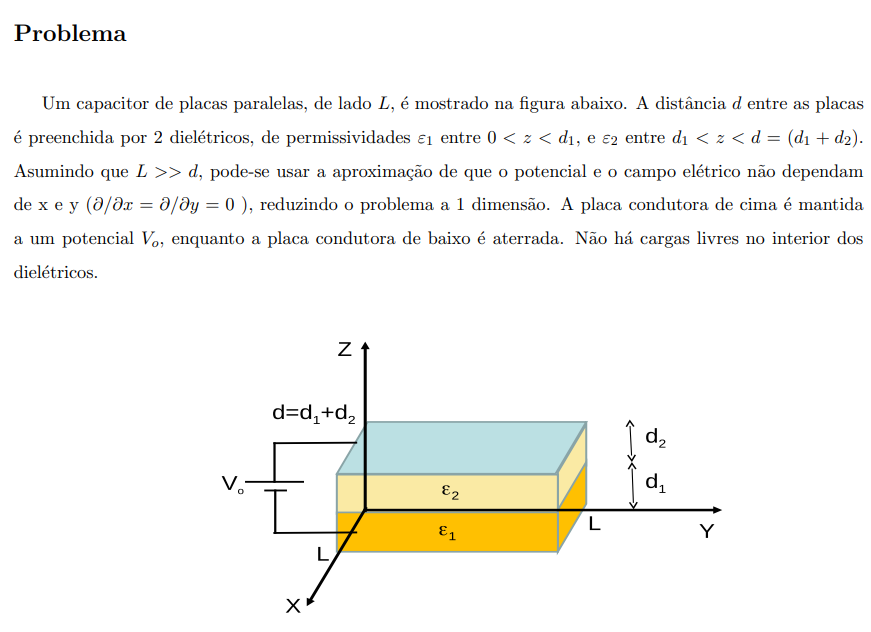
\includegraphics[width=15cm,height=15cm]{Enunciado/Enunciado.png}}
    \label{fig:dale}
    \end{figure}

    \subsection{Solução pelo Metodo dos Elementos Finitos - 1D}
    \begin{itemize}
    \item O primeiro passo para resolver o problema proposto no projeto é realizar a análise do domínio do problema afim de discretizar o domínio em questão. 
    \item Em seguida, o método dos elementos finitos em uma dimensão (FEM - 1D) será aplicado a fim de obter o sistema matricial linear que representa o domínio do problema.
    \item Por fim, uma vez obtido o sistema matricial linear equivalente ao domínio do problema, serão aplicadas as condições de contorno de Dirichlet adequadas.
    \item Segue abaixo a formulação matemática para chegar no resultado desejado:
    \end{itemize}
    
    
    \begin{figure}[!htb]
    \centerline{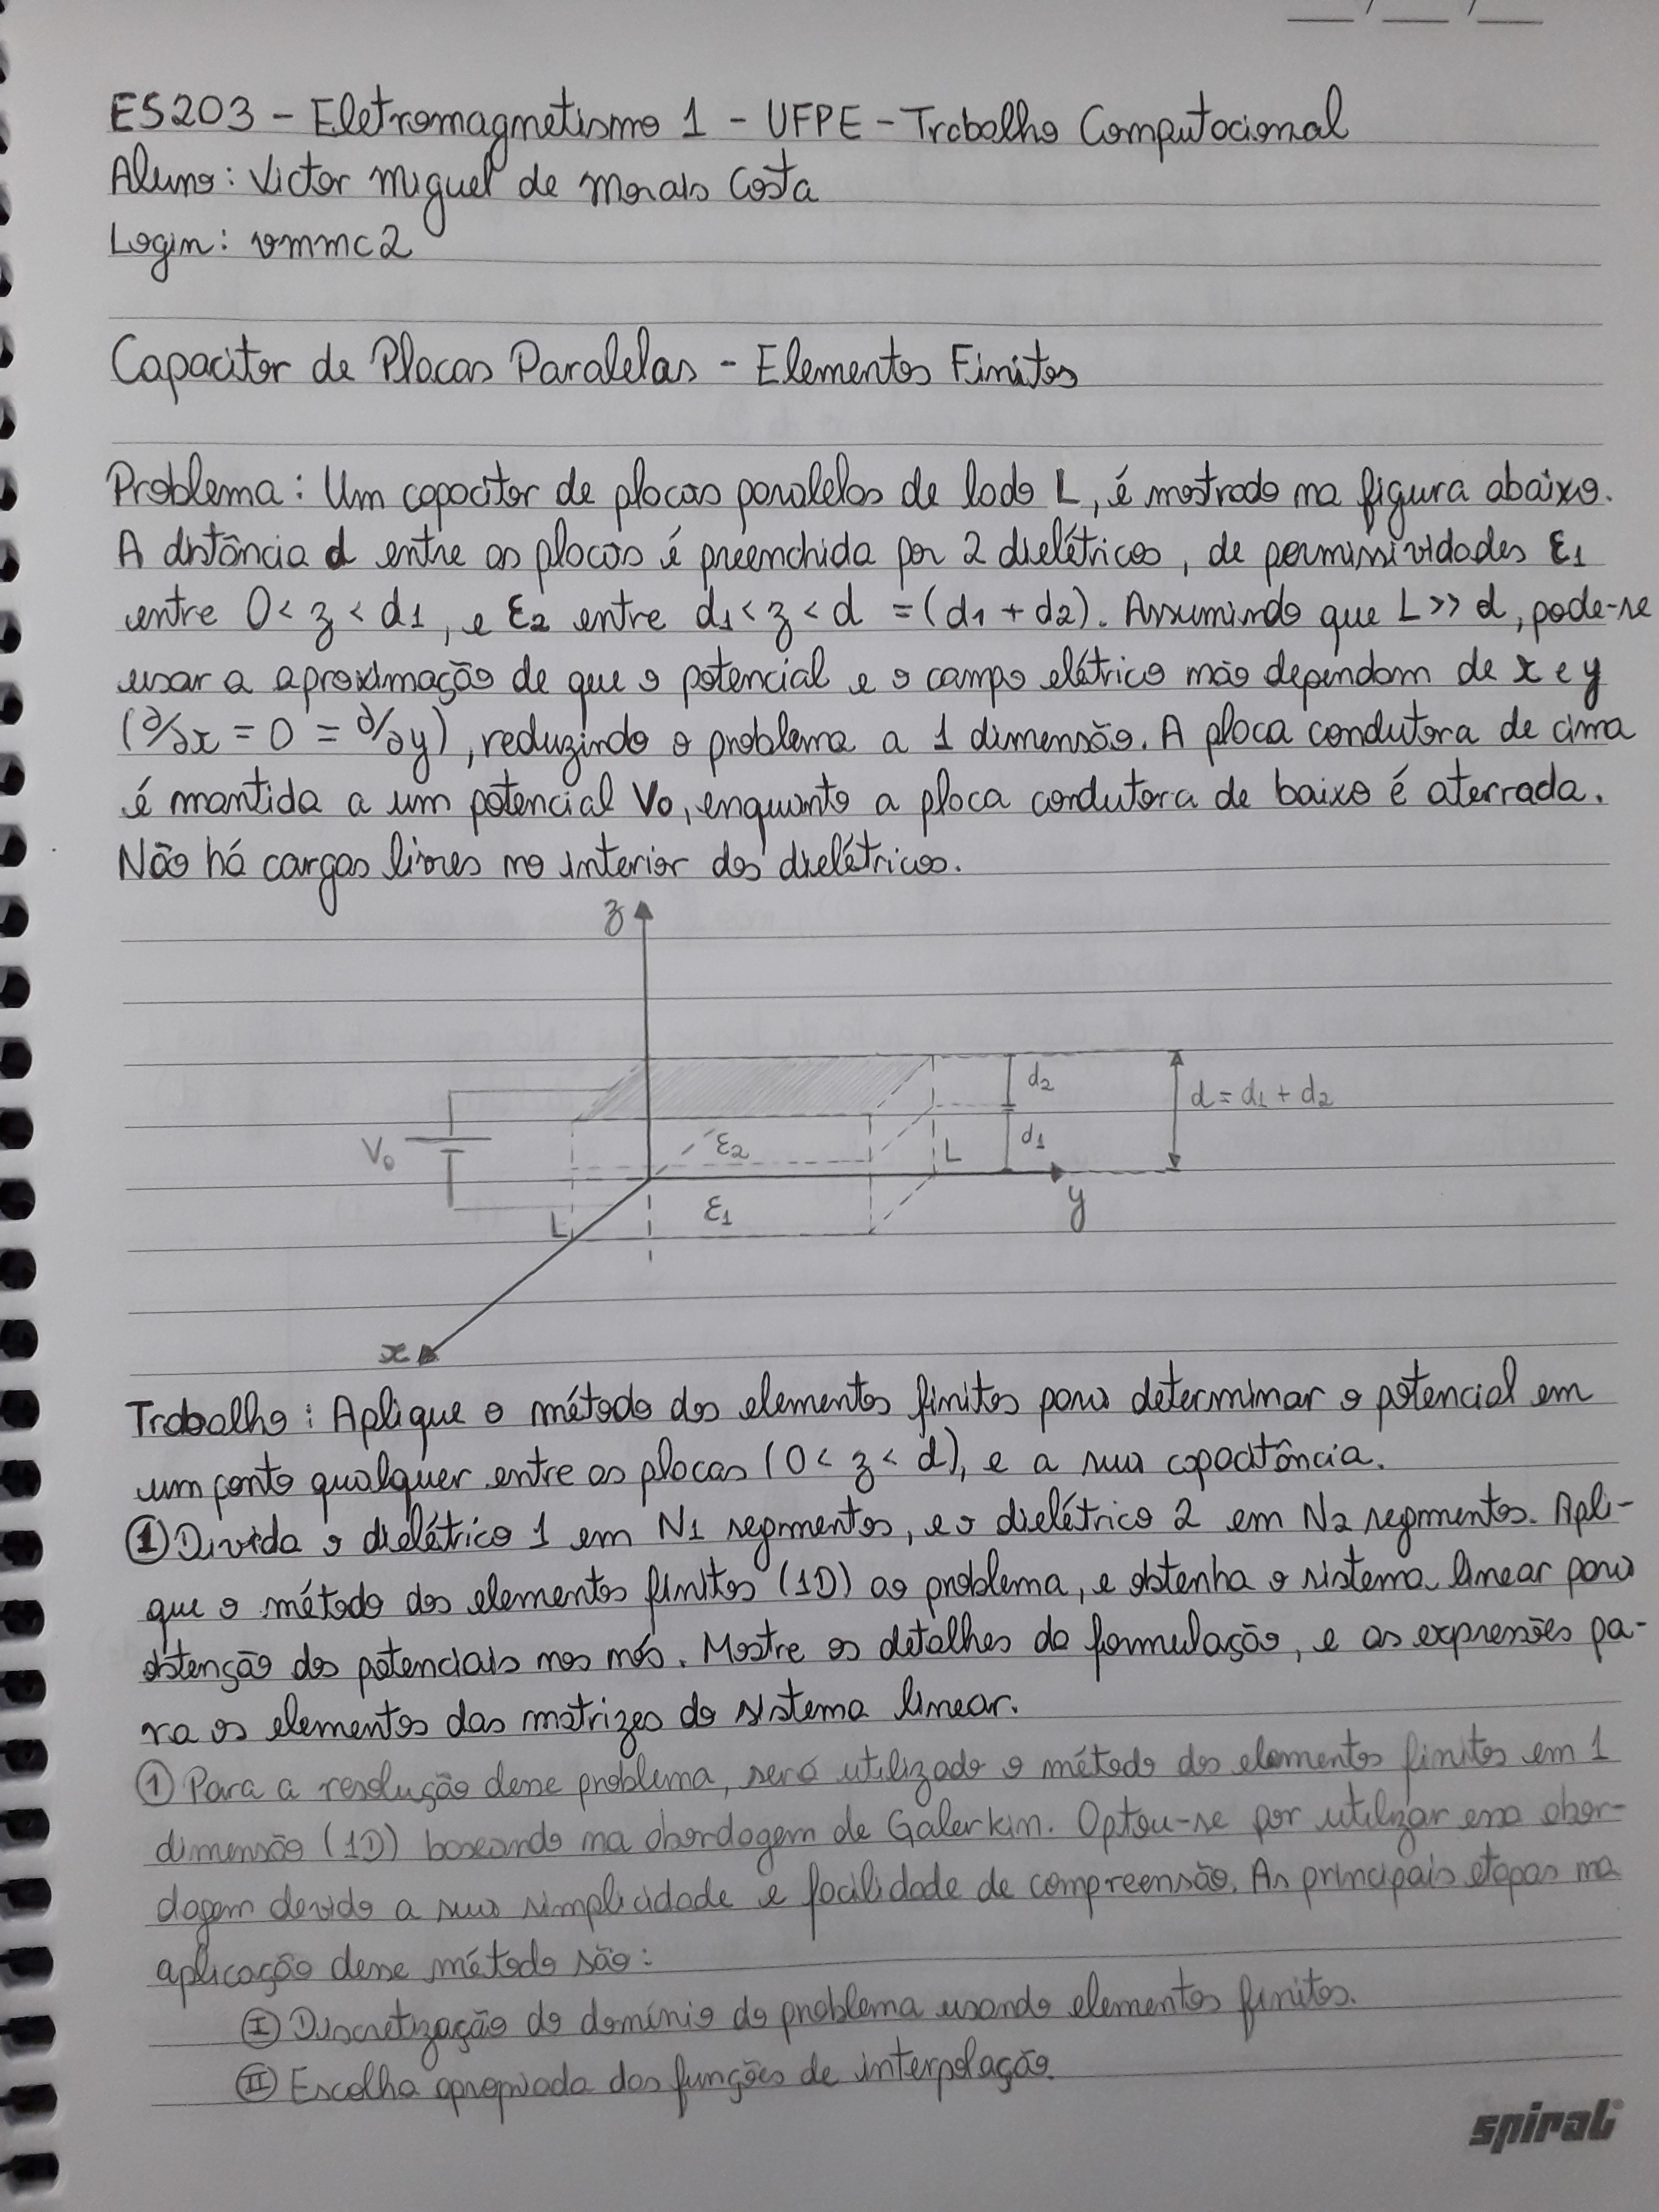
\includegraphics[width=20cm,height=22cm]{Formulação Matemática/Formulacao - Parte 1.jpg}}
    \caption{Formulação - Parte 1}
    \label{fig:fp1}
    \end{figure}
    
    \begin{figure}[!htb]
    \centerline{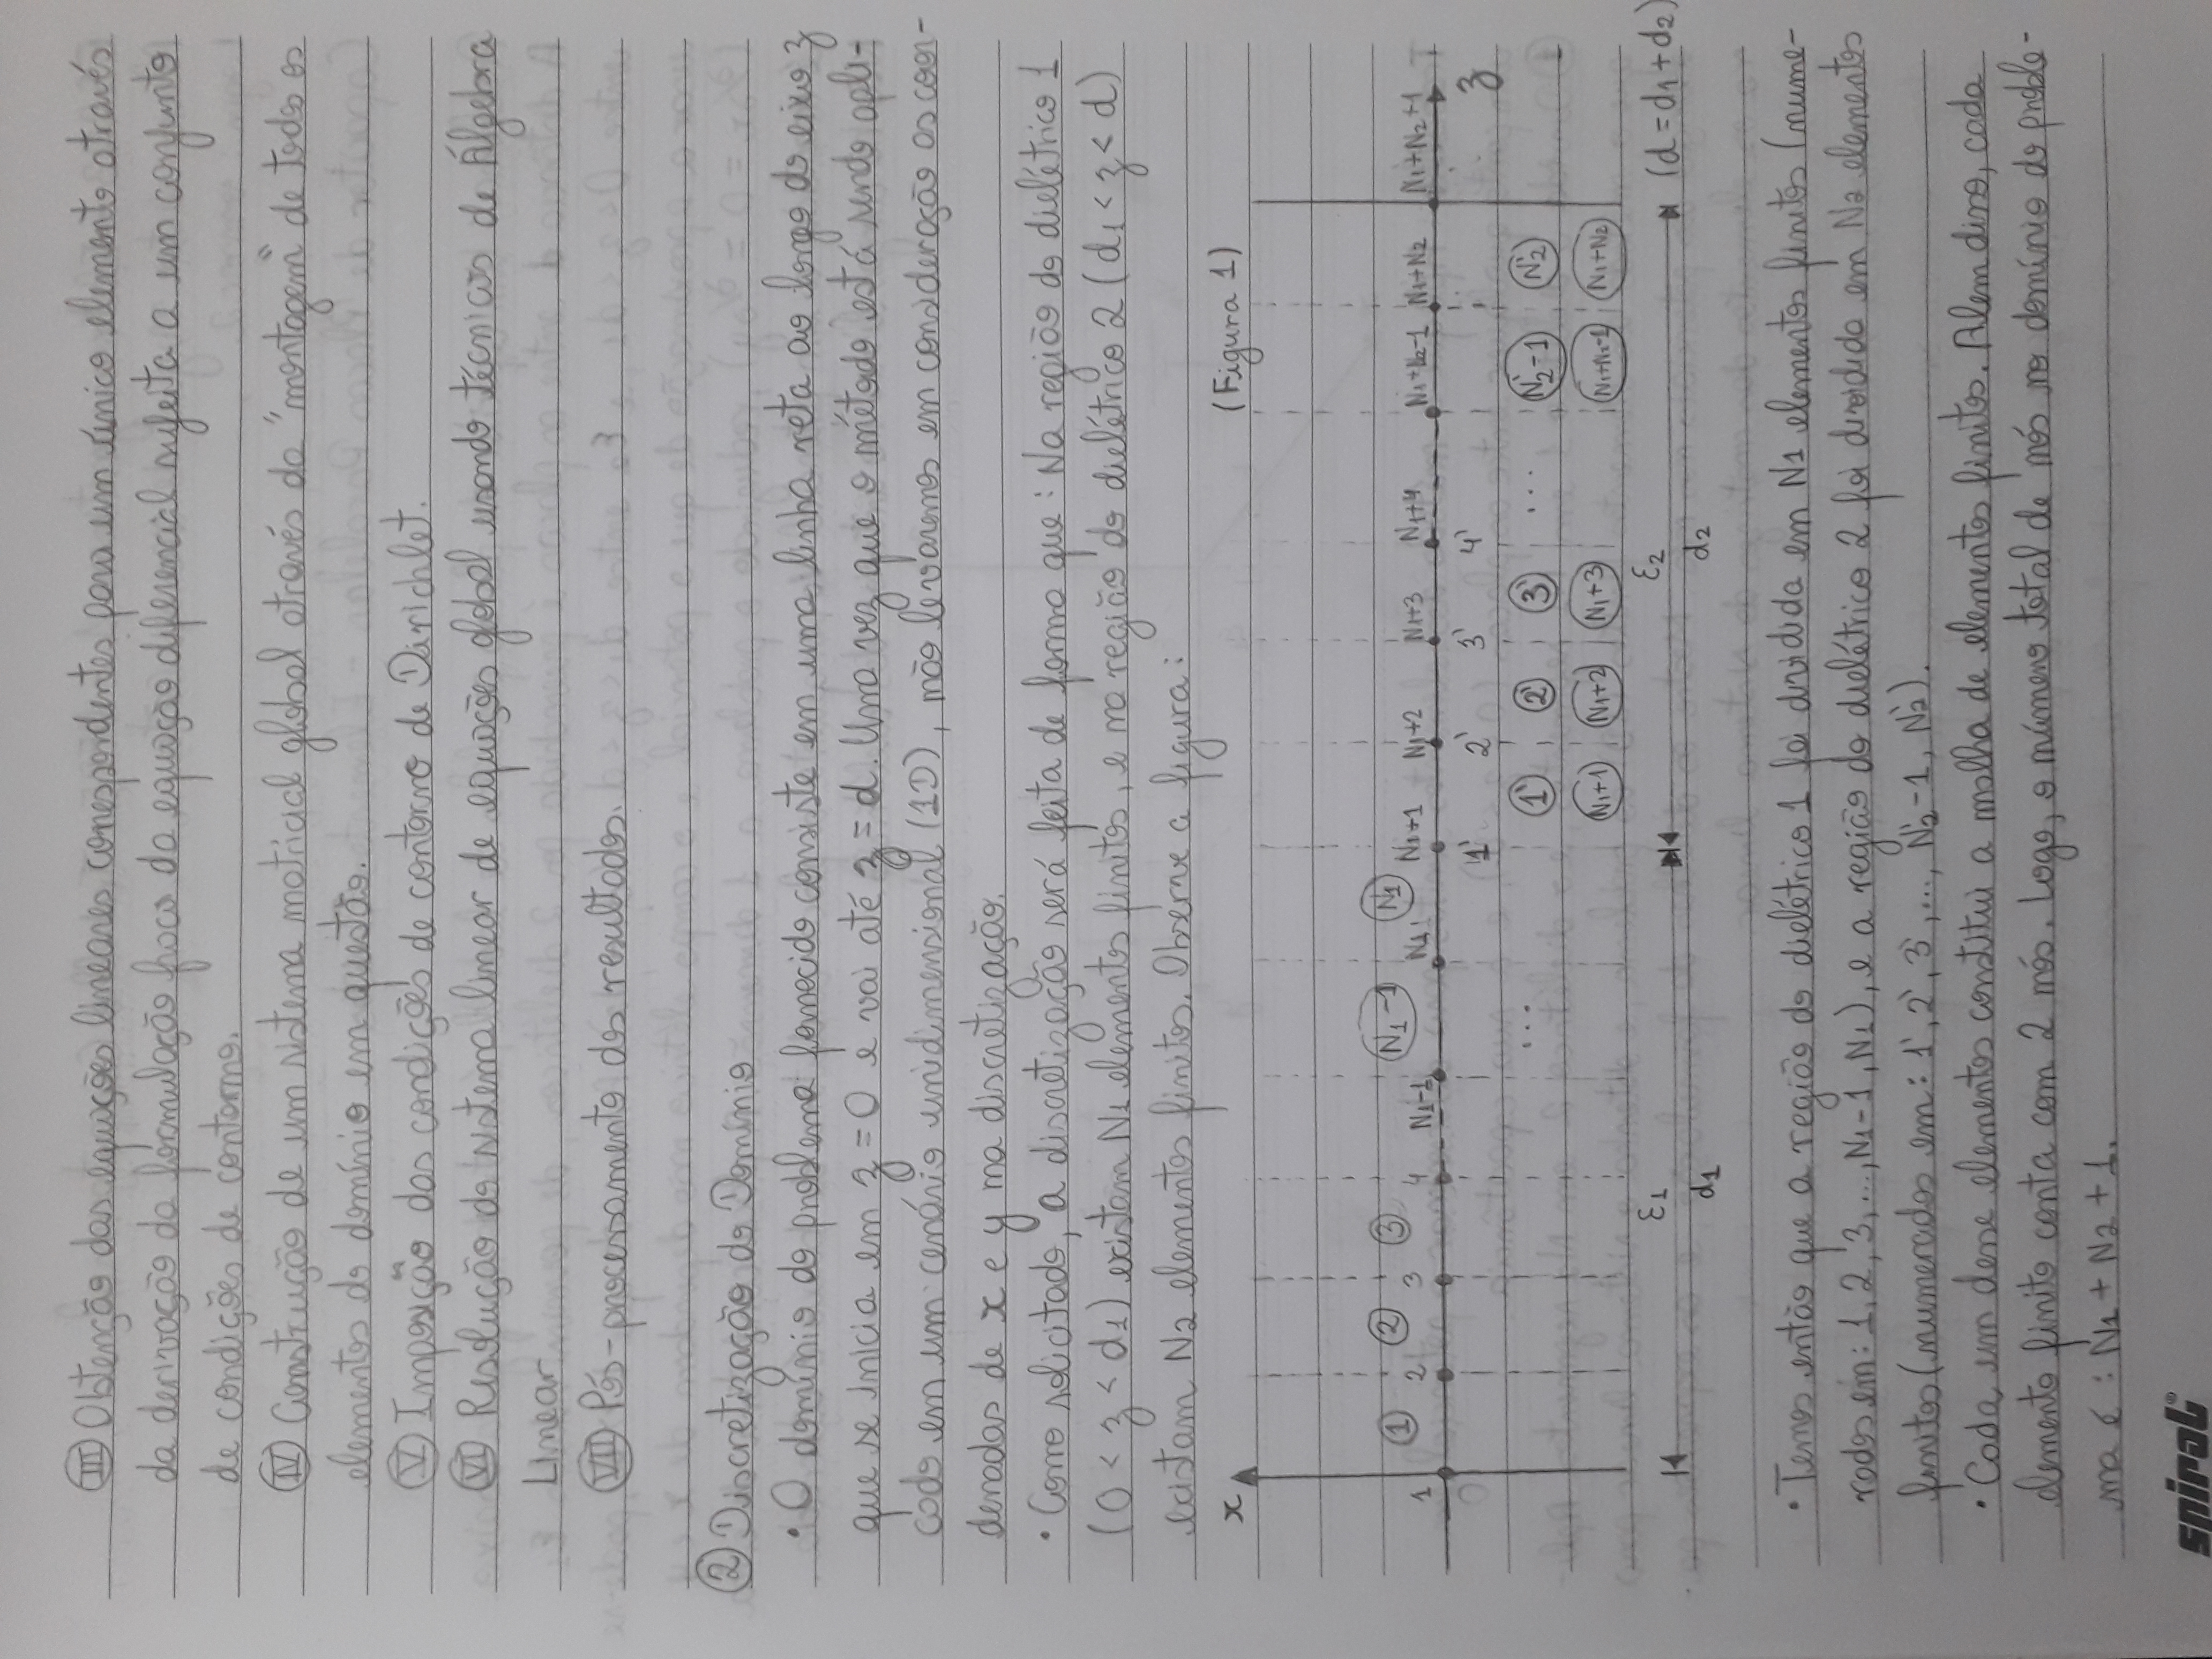
\includegraphics[width=20cm,height=22cm]{Formulação Matemática/Formulacao - Parte 2.jpg}}
    \caption{Formulação - Parte 2}
    \label{fig:fp2}
    \end{figure}
    
    \begin{figure}[!htb]
    \centerline{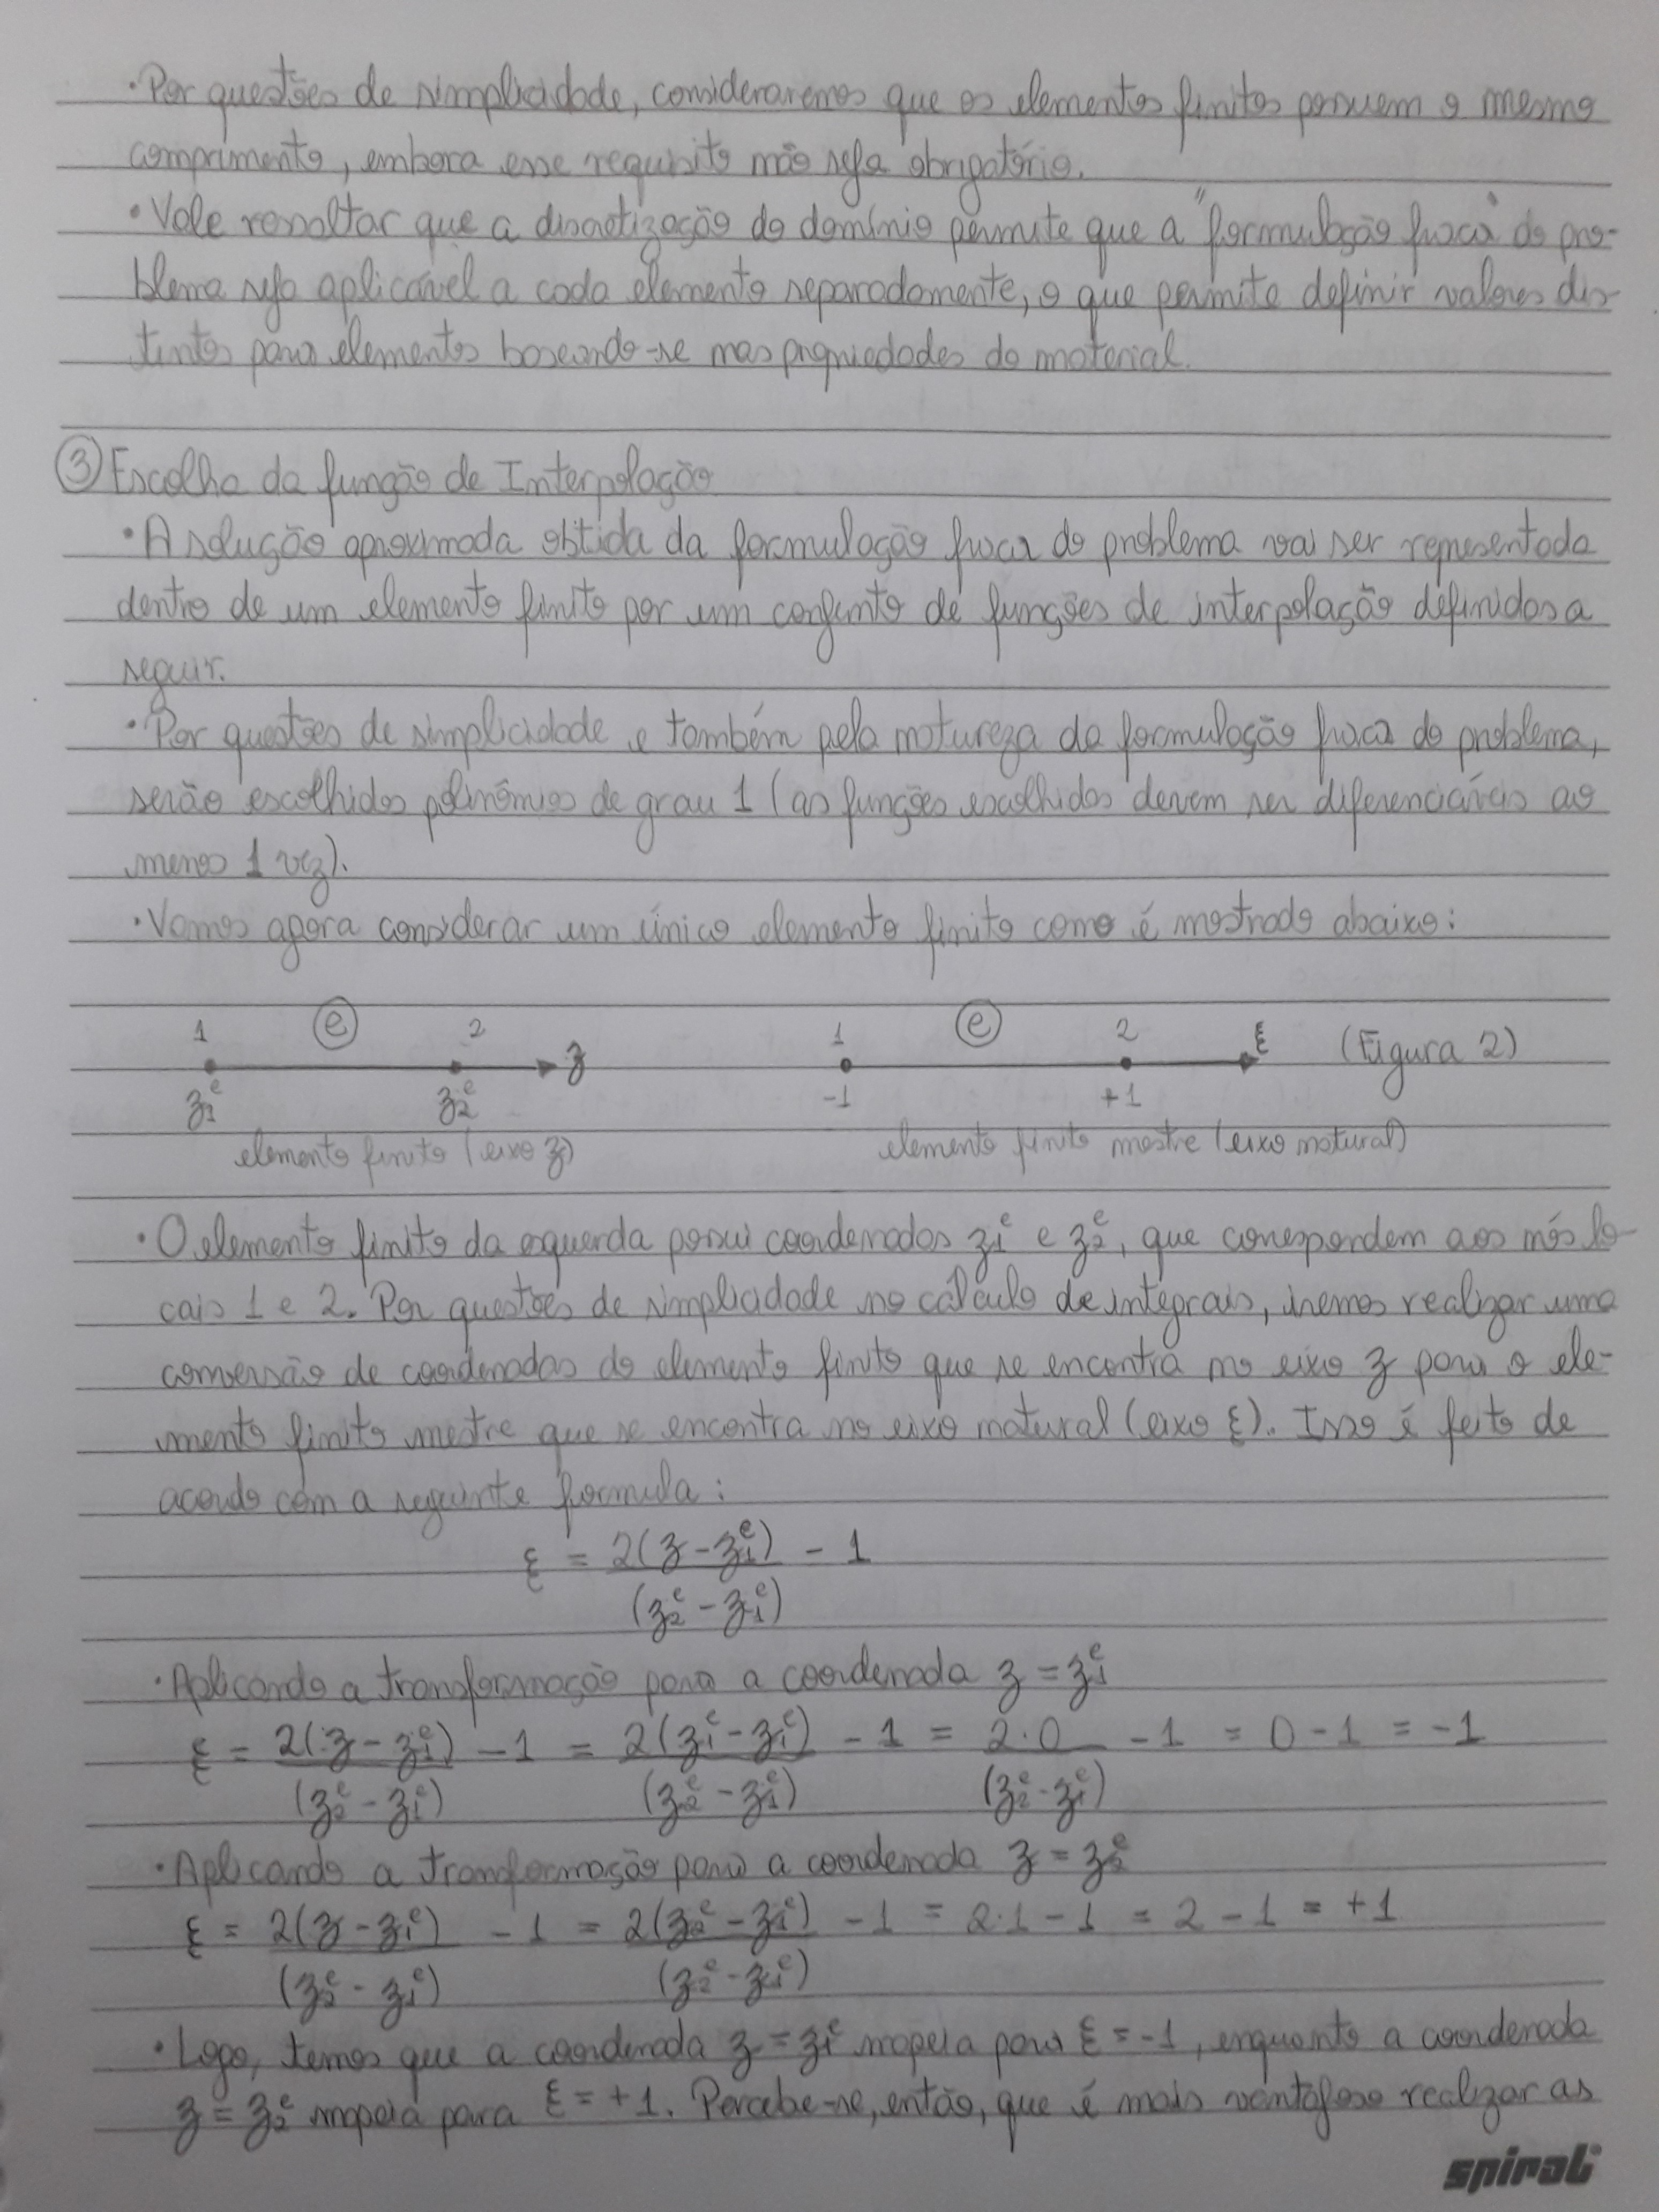
\includegraphics[width=20cm,height=22cm]{Formulação Matemática/Formulacao - Parte 3.jpg}}
    \caption{Formulação - Parte 3}
    \label{fig:fp3}
    \end{figure}
    
    \begin{figure}[!htb]
    \centerline{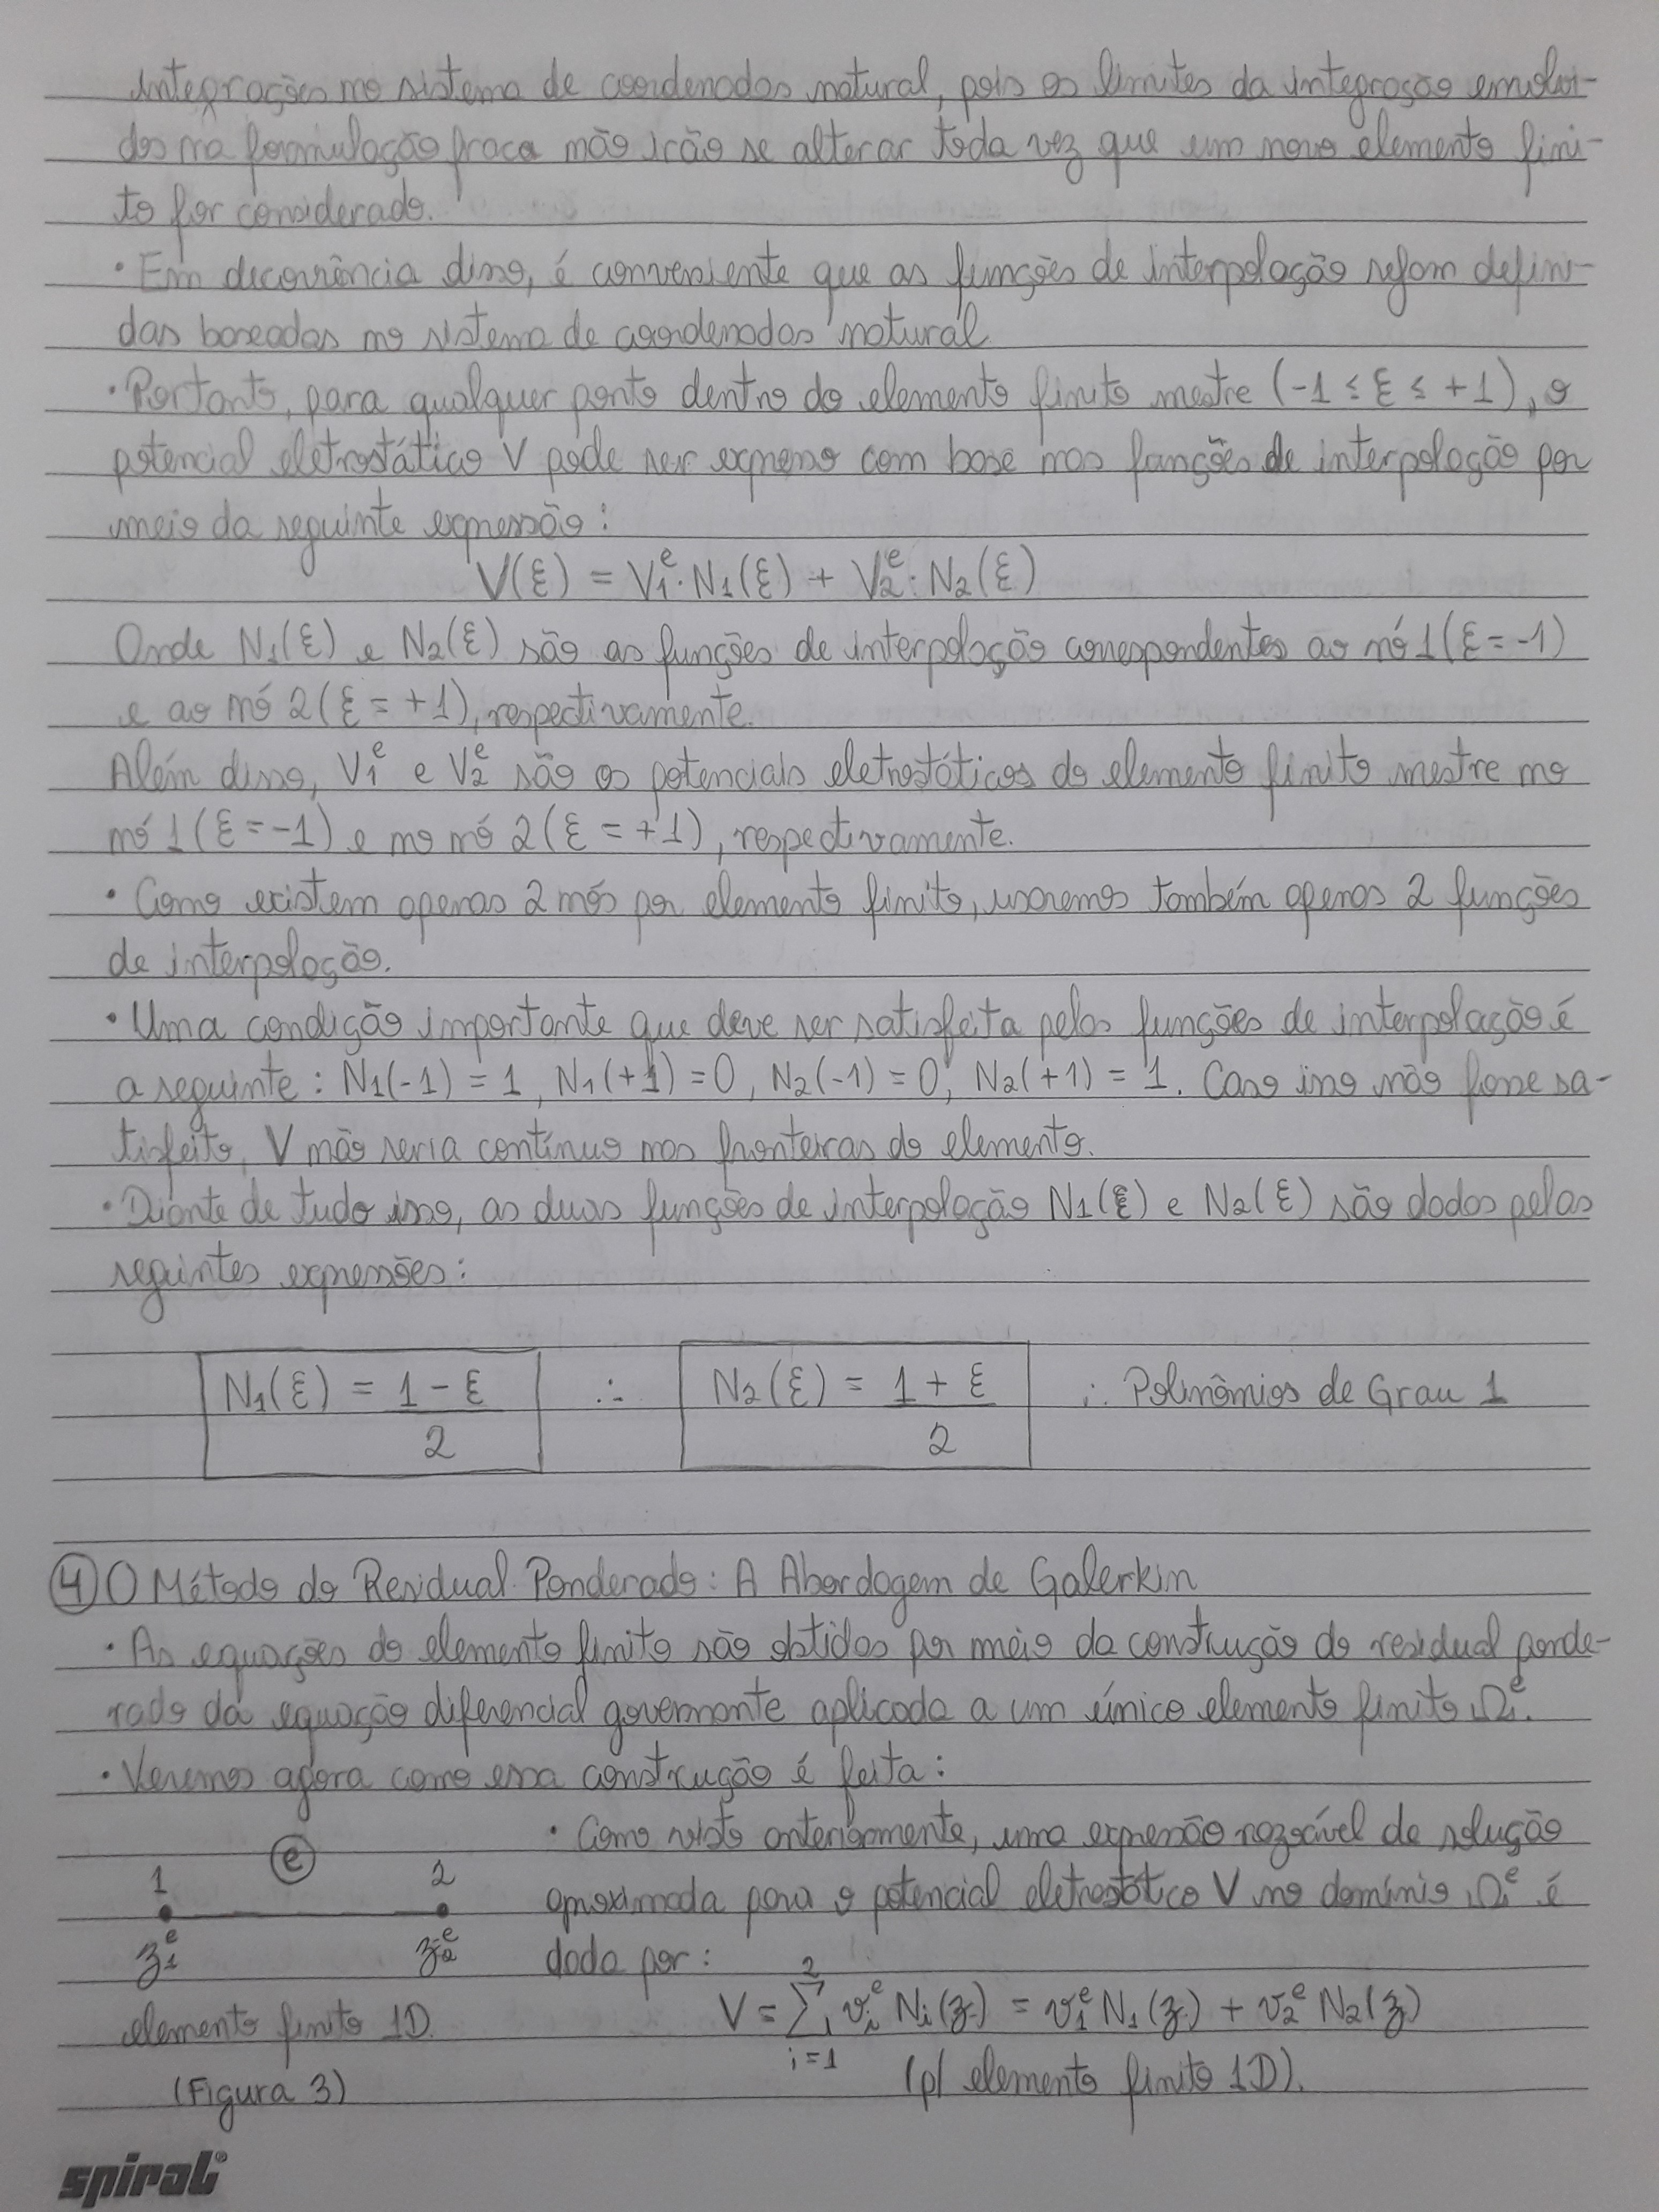
\includegraphics[width=20cm,height=22cm]{Formulação Matemática/Formulacao - Parte 4.jpg}}
    \caption{Formulação - Parte 4}
    \label{fig:fp4}
    \end{figure}
    
    \begin{figure}[!htb]
    \centerline{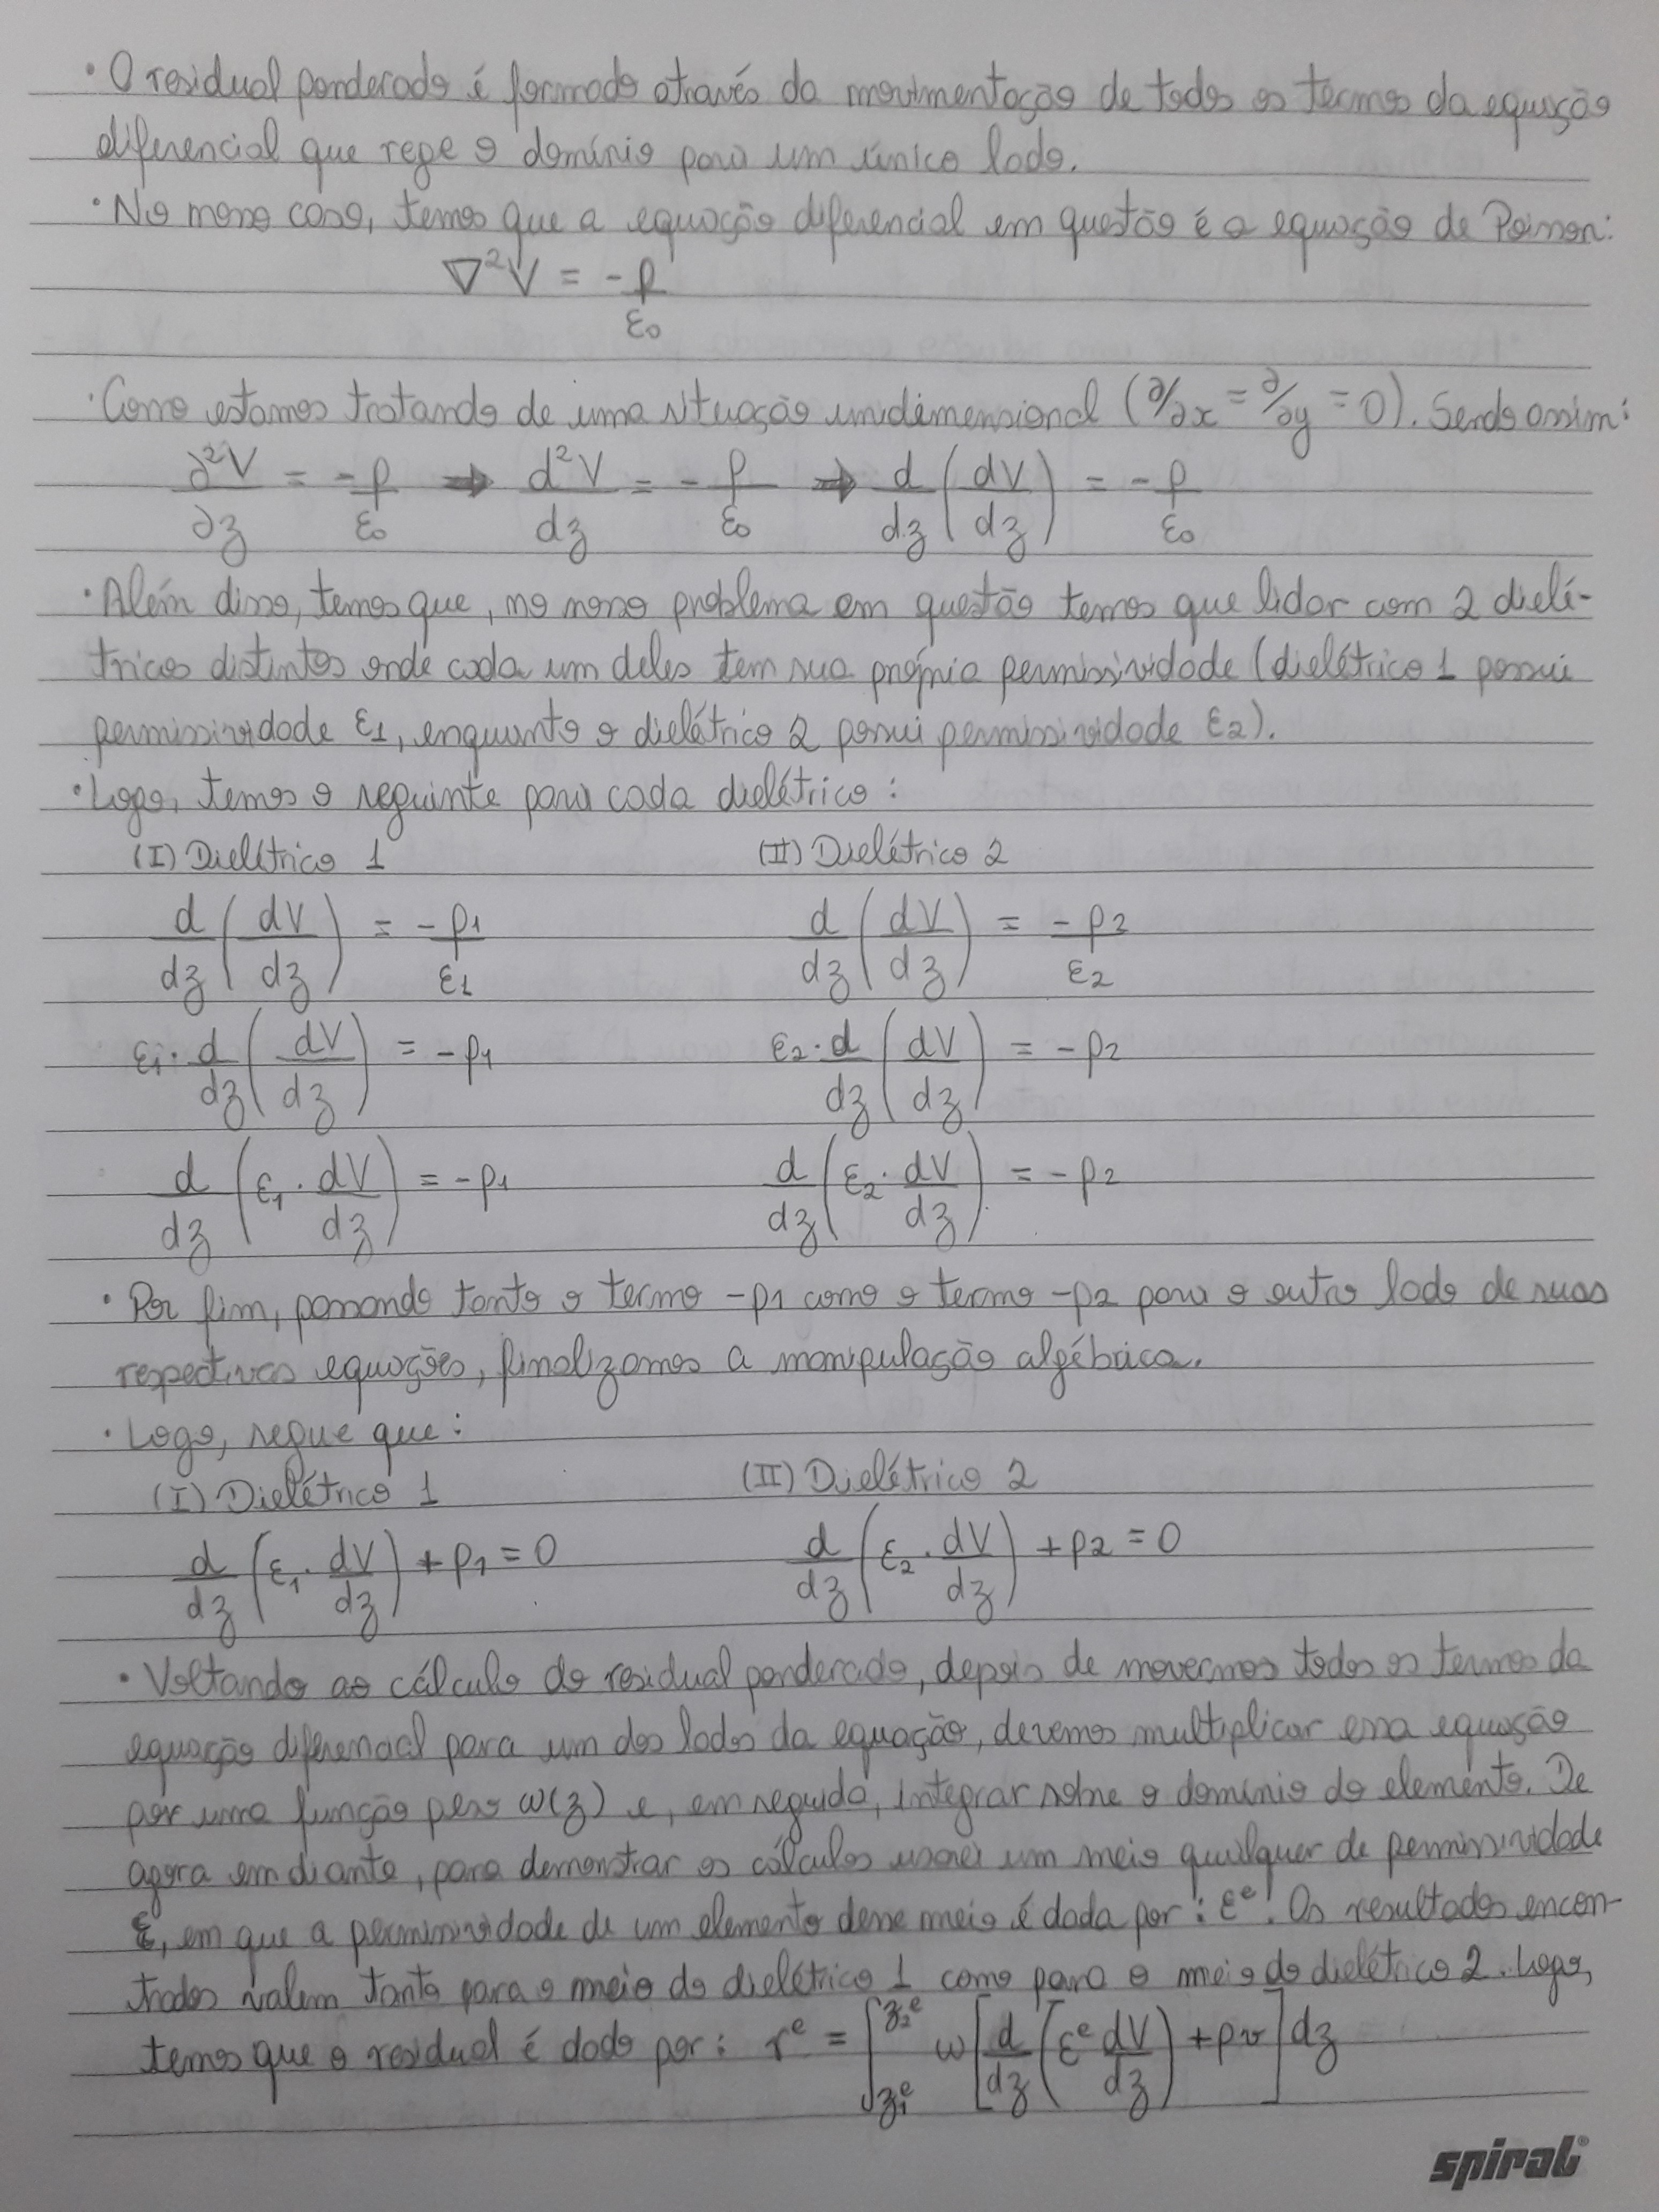
\includegraphics[width=20cm,height=22cm]{Formulação Matemática/Formulacao - Parte 5.jpg}}
    \caption{Formulação - Parte 5}
    \label{fig:fp5}
    \end{figure}
    
    \begin{figure}[!htb]
    \centerline{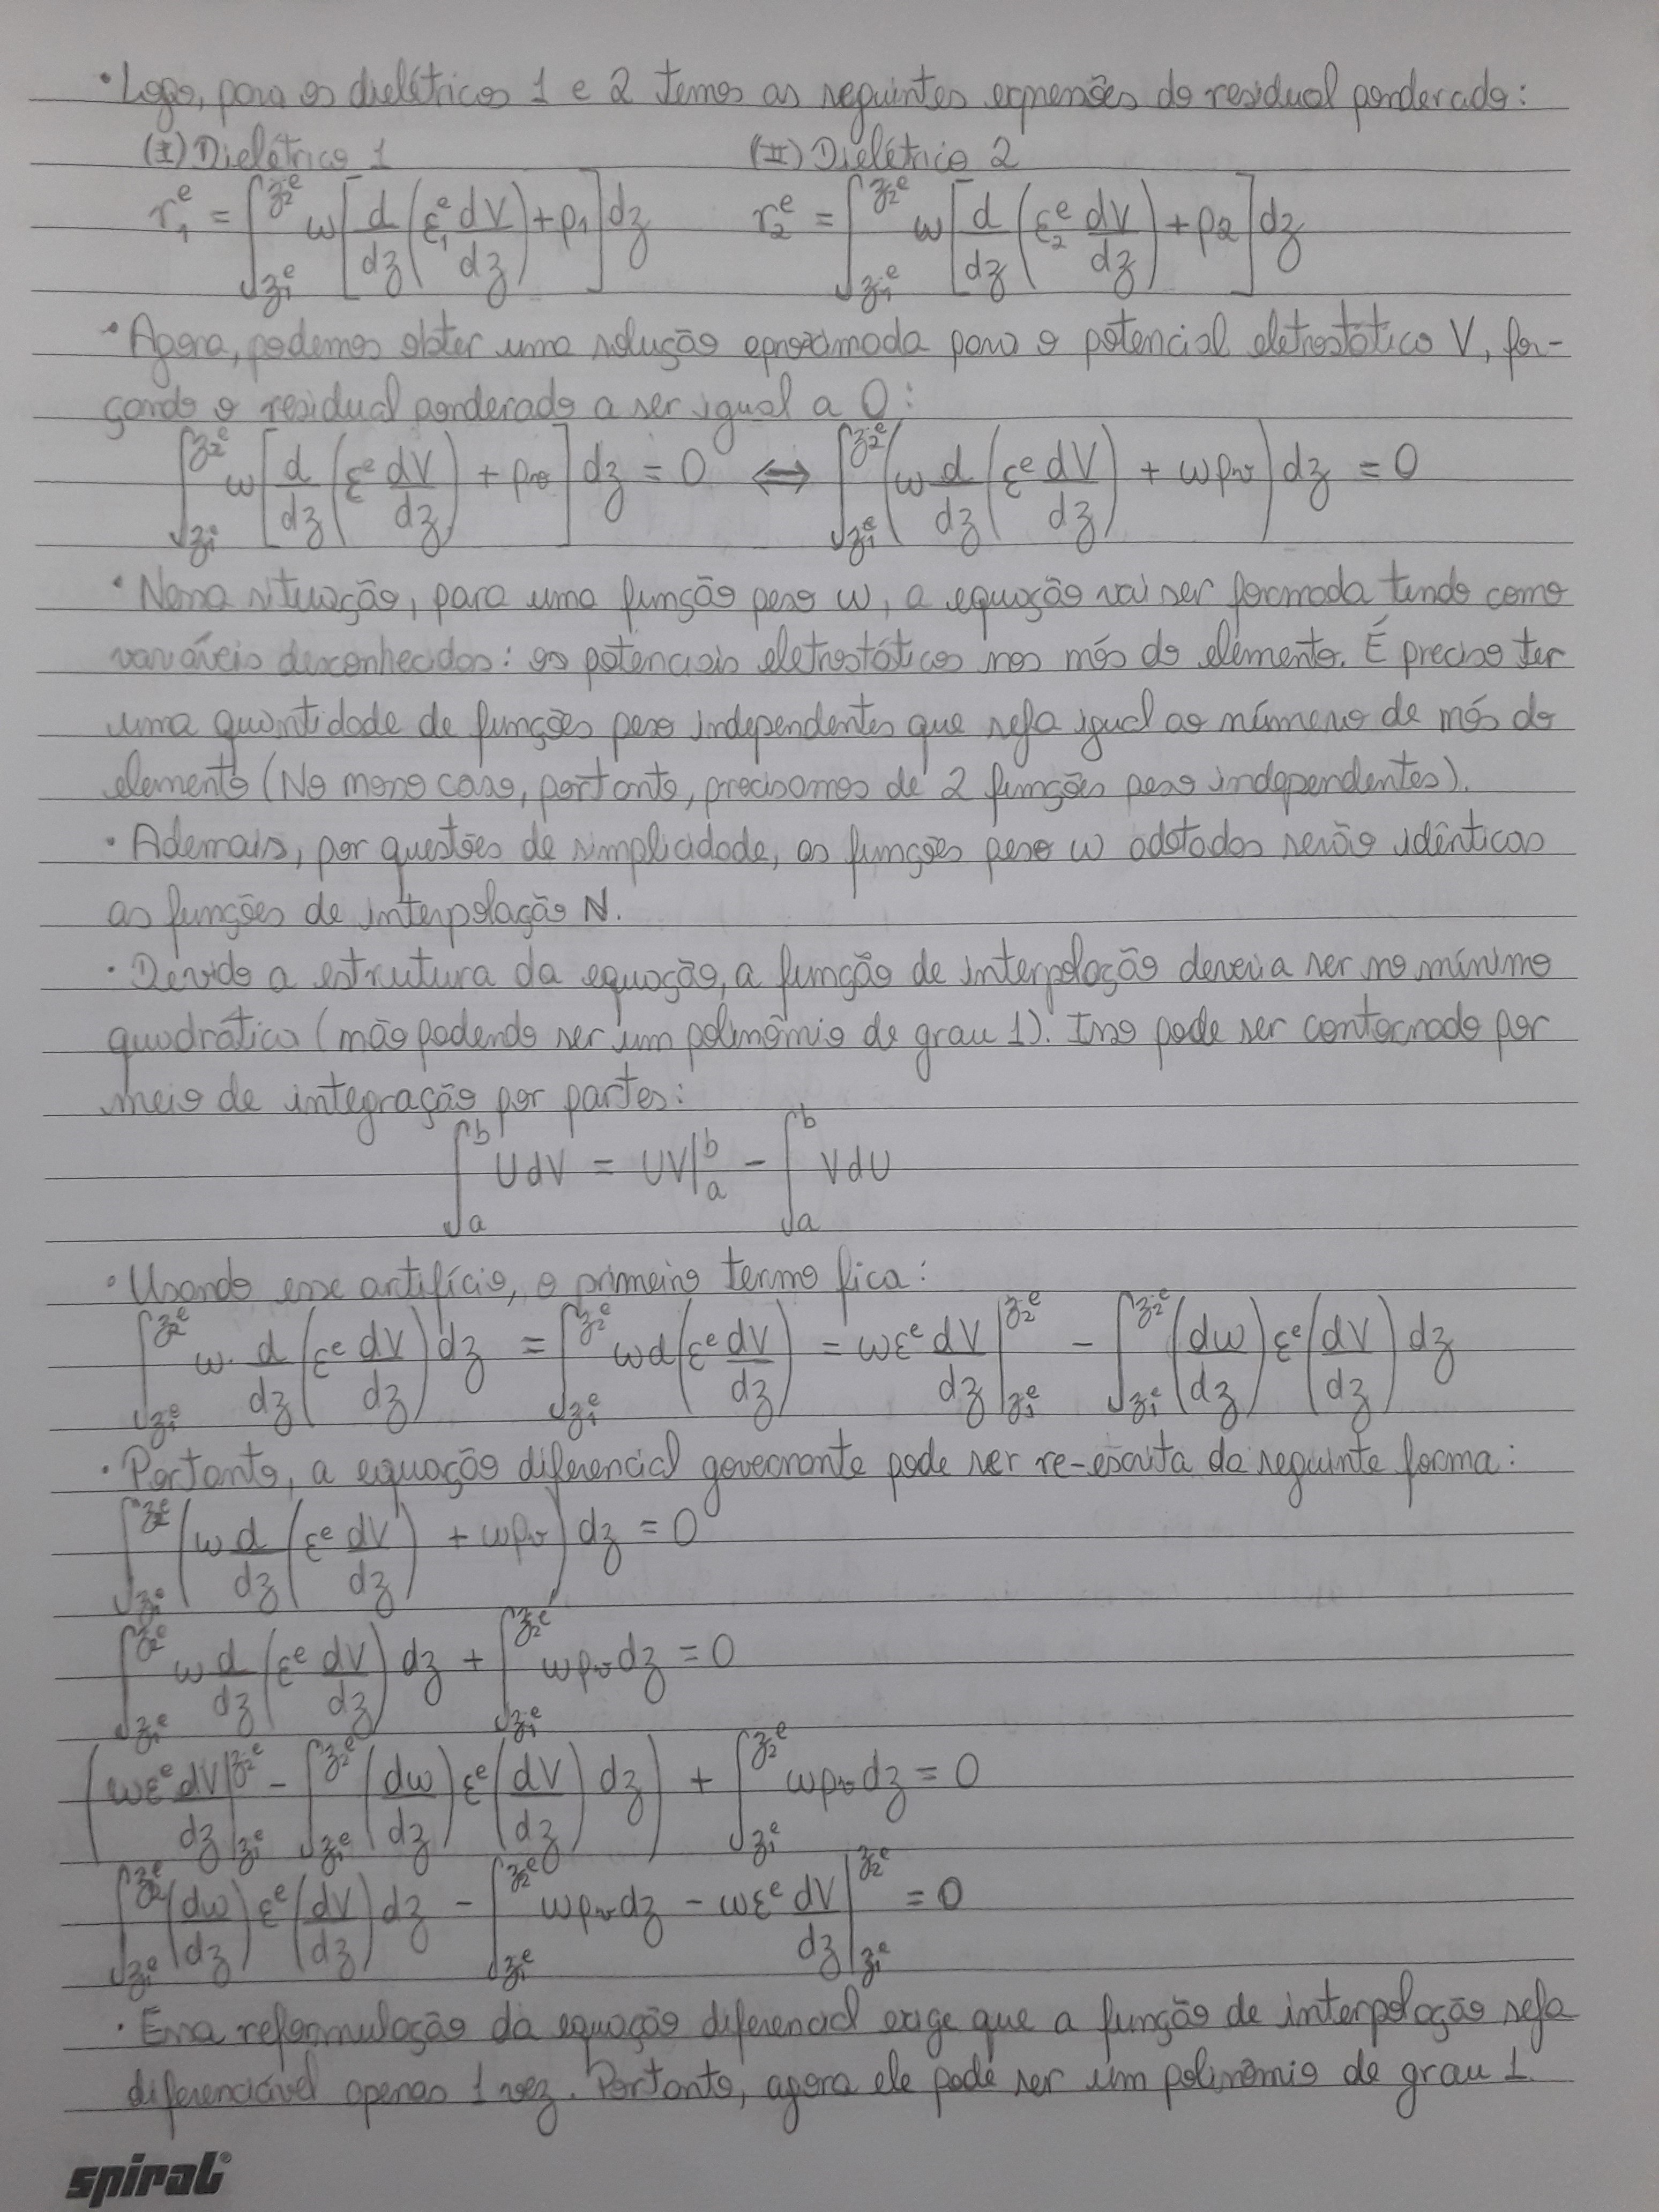
\includegraphics[width=20cm,height=22cm]{Formulação Matemática/Formulacao - Parte 6.jpg}}
    \caption{Formulação - Parte 6}
    \label{fig:fp6}
    \end{figure}
    
    \begin{figure}[!htb]
    \centerline{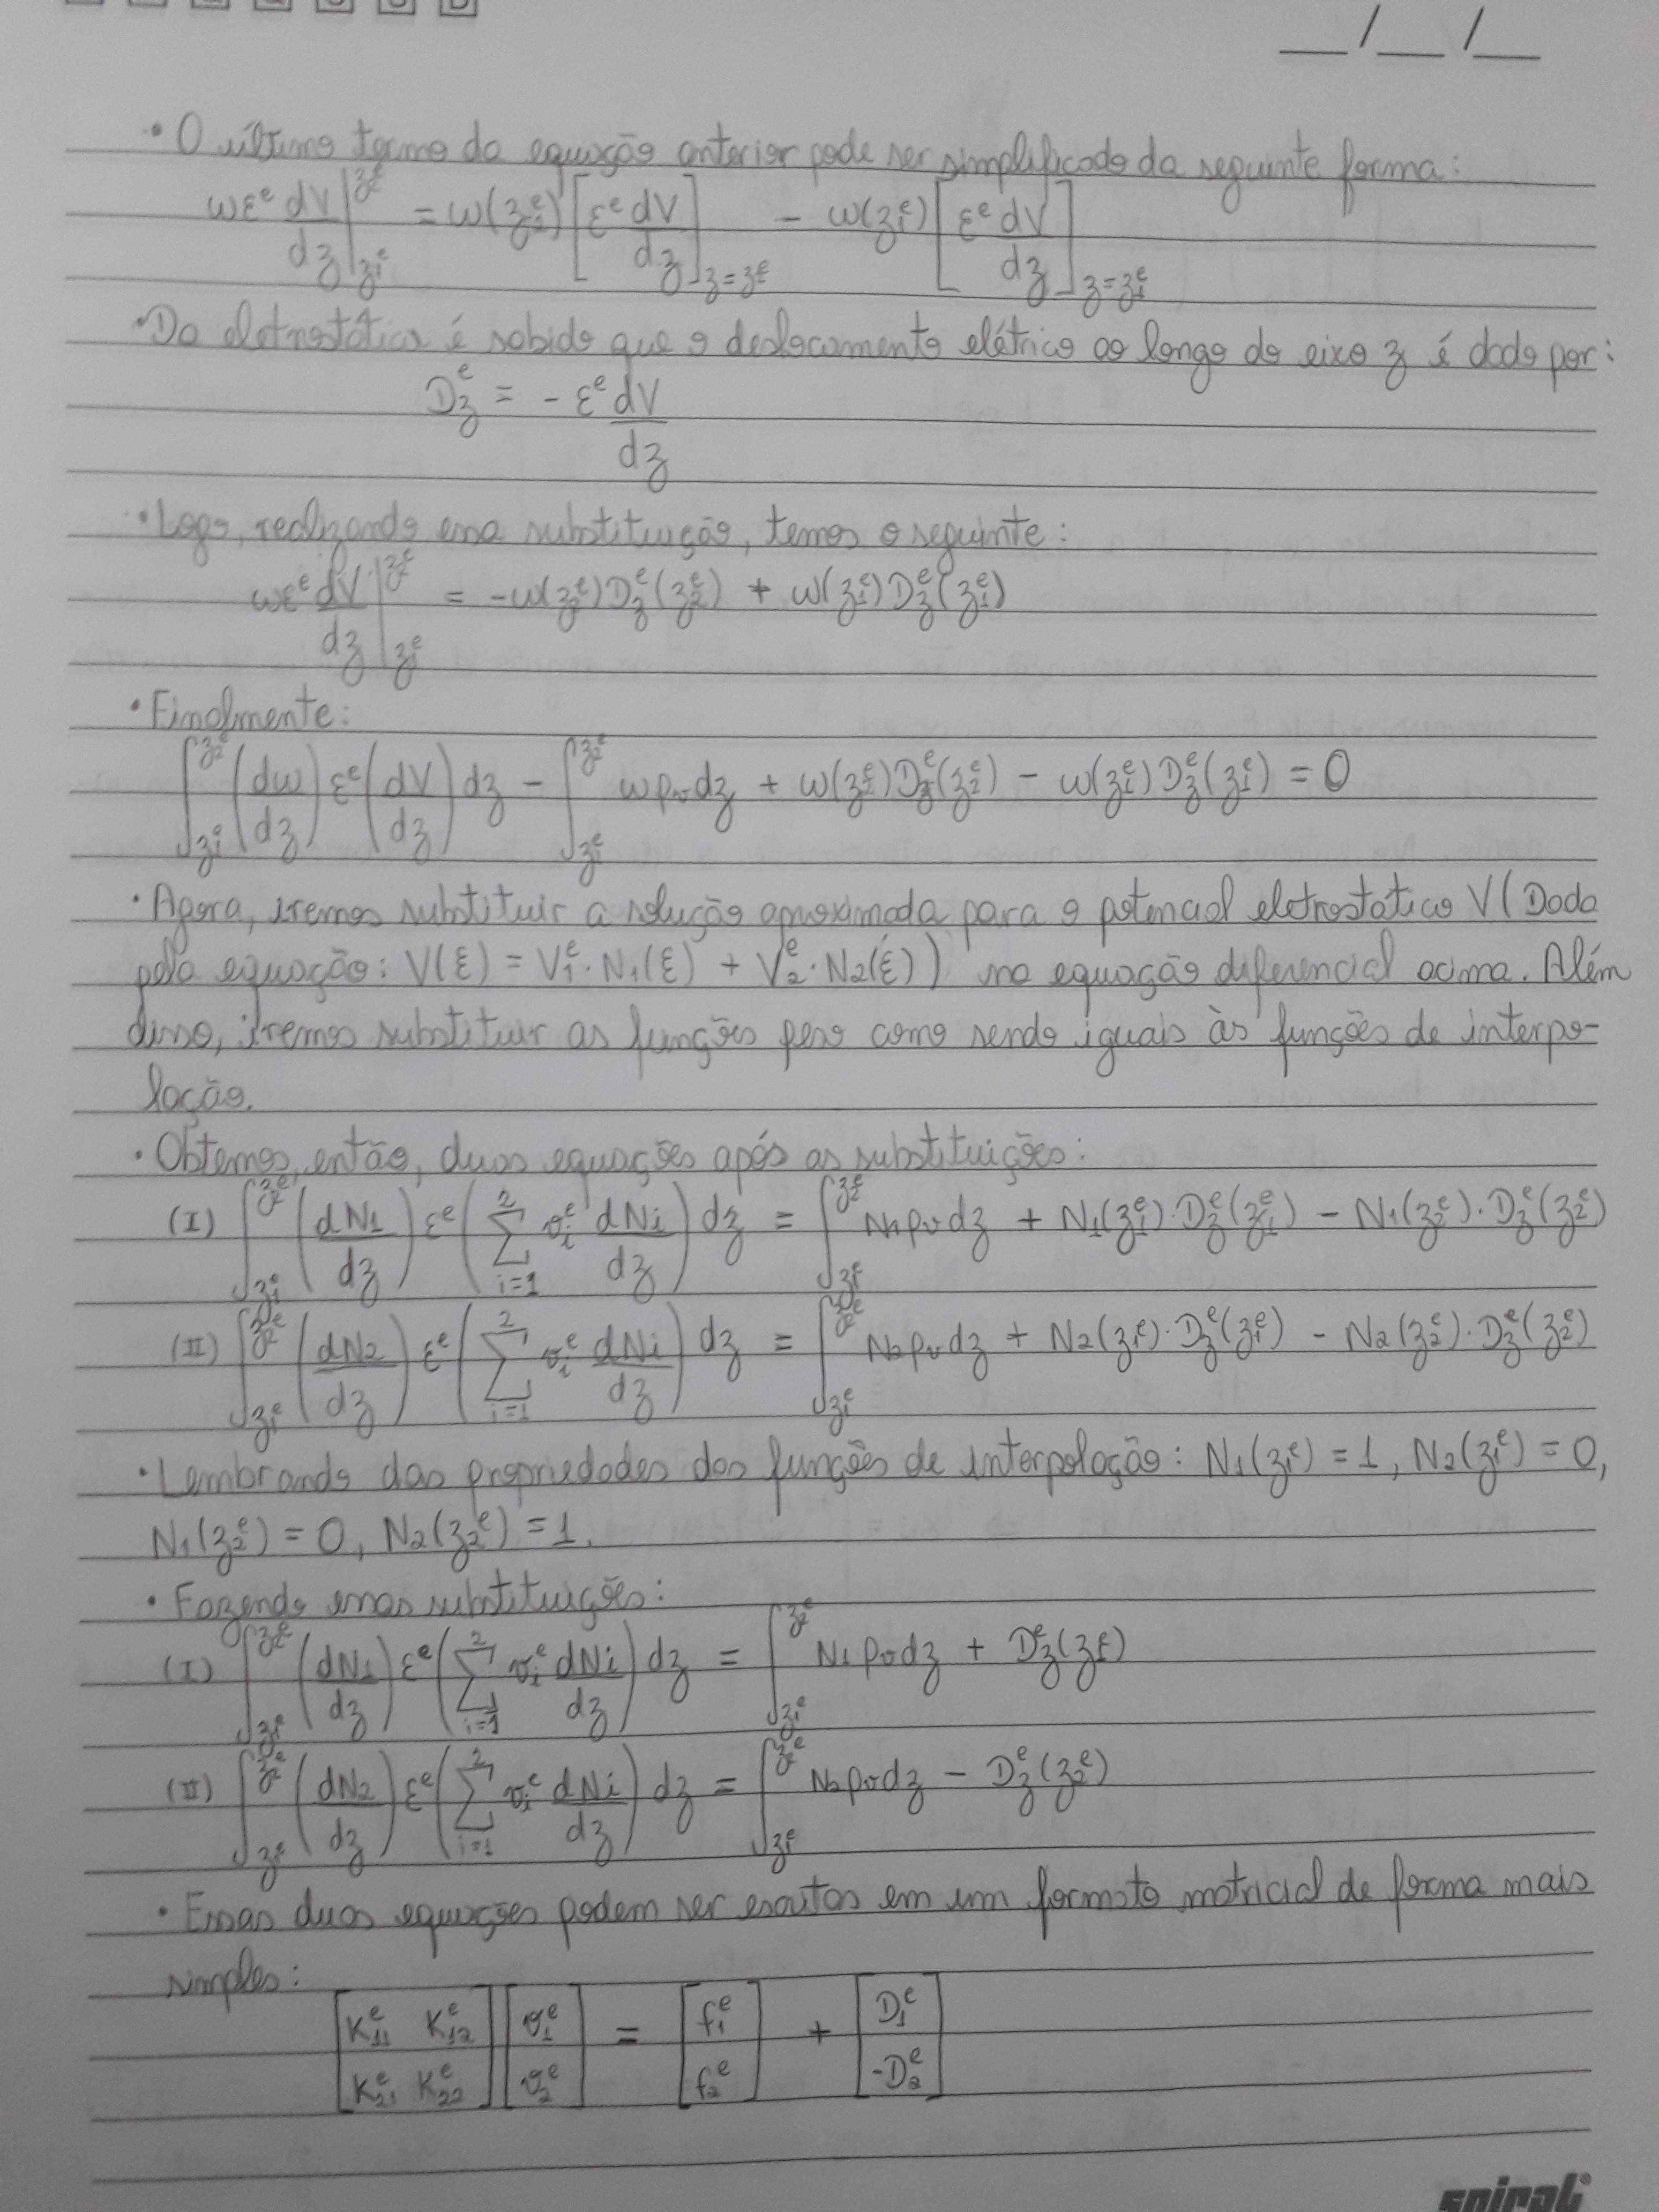
\includegraphics[width=20cm,height=22cm]{Formulação Matemática/Formulacao - Parte 7.jpg}}
    \caption{Formulação - Parte 7}
    \label{fig:fp7}
    \end{figure}
    
    \begin{figure}[!htb]
    \centerline{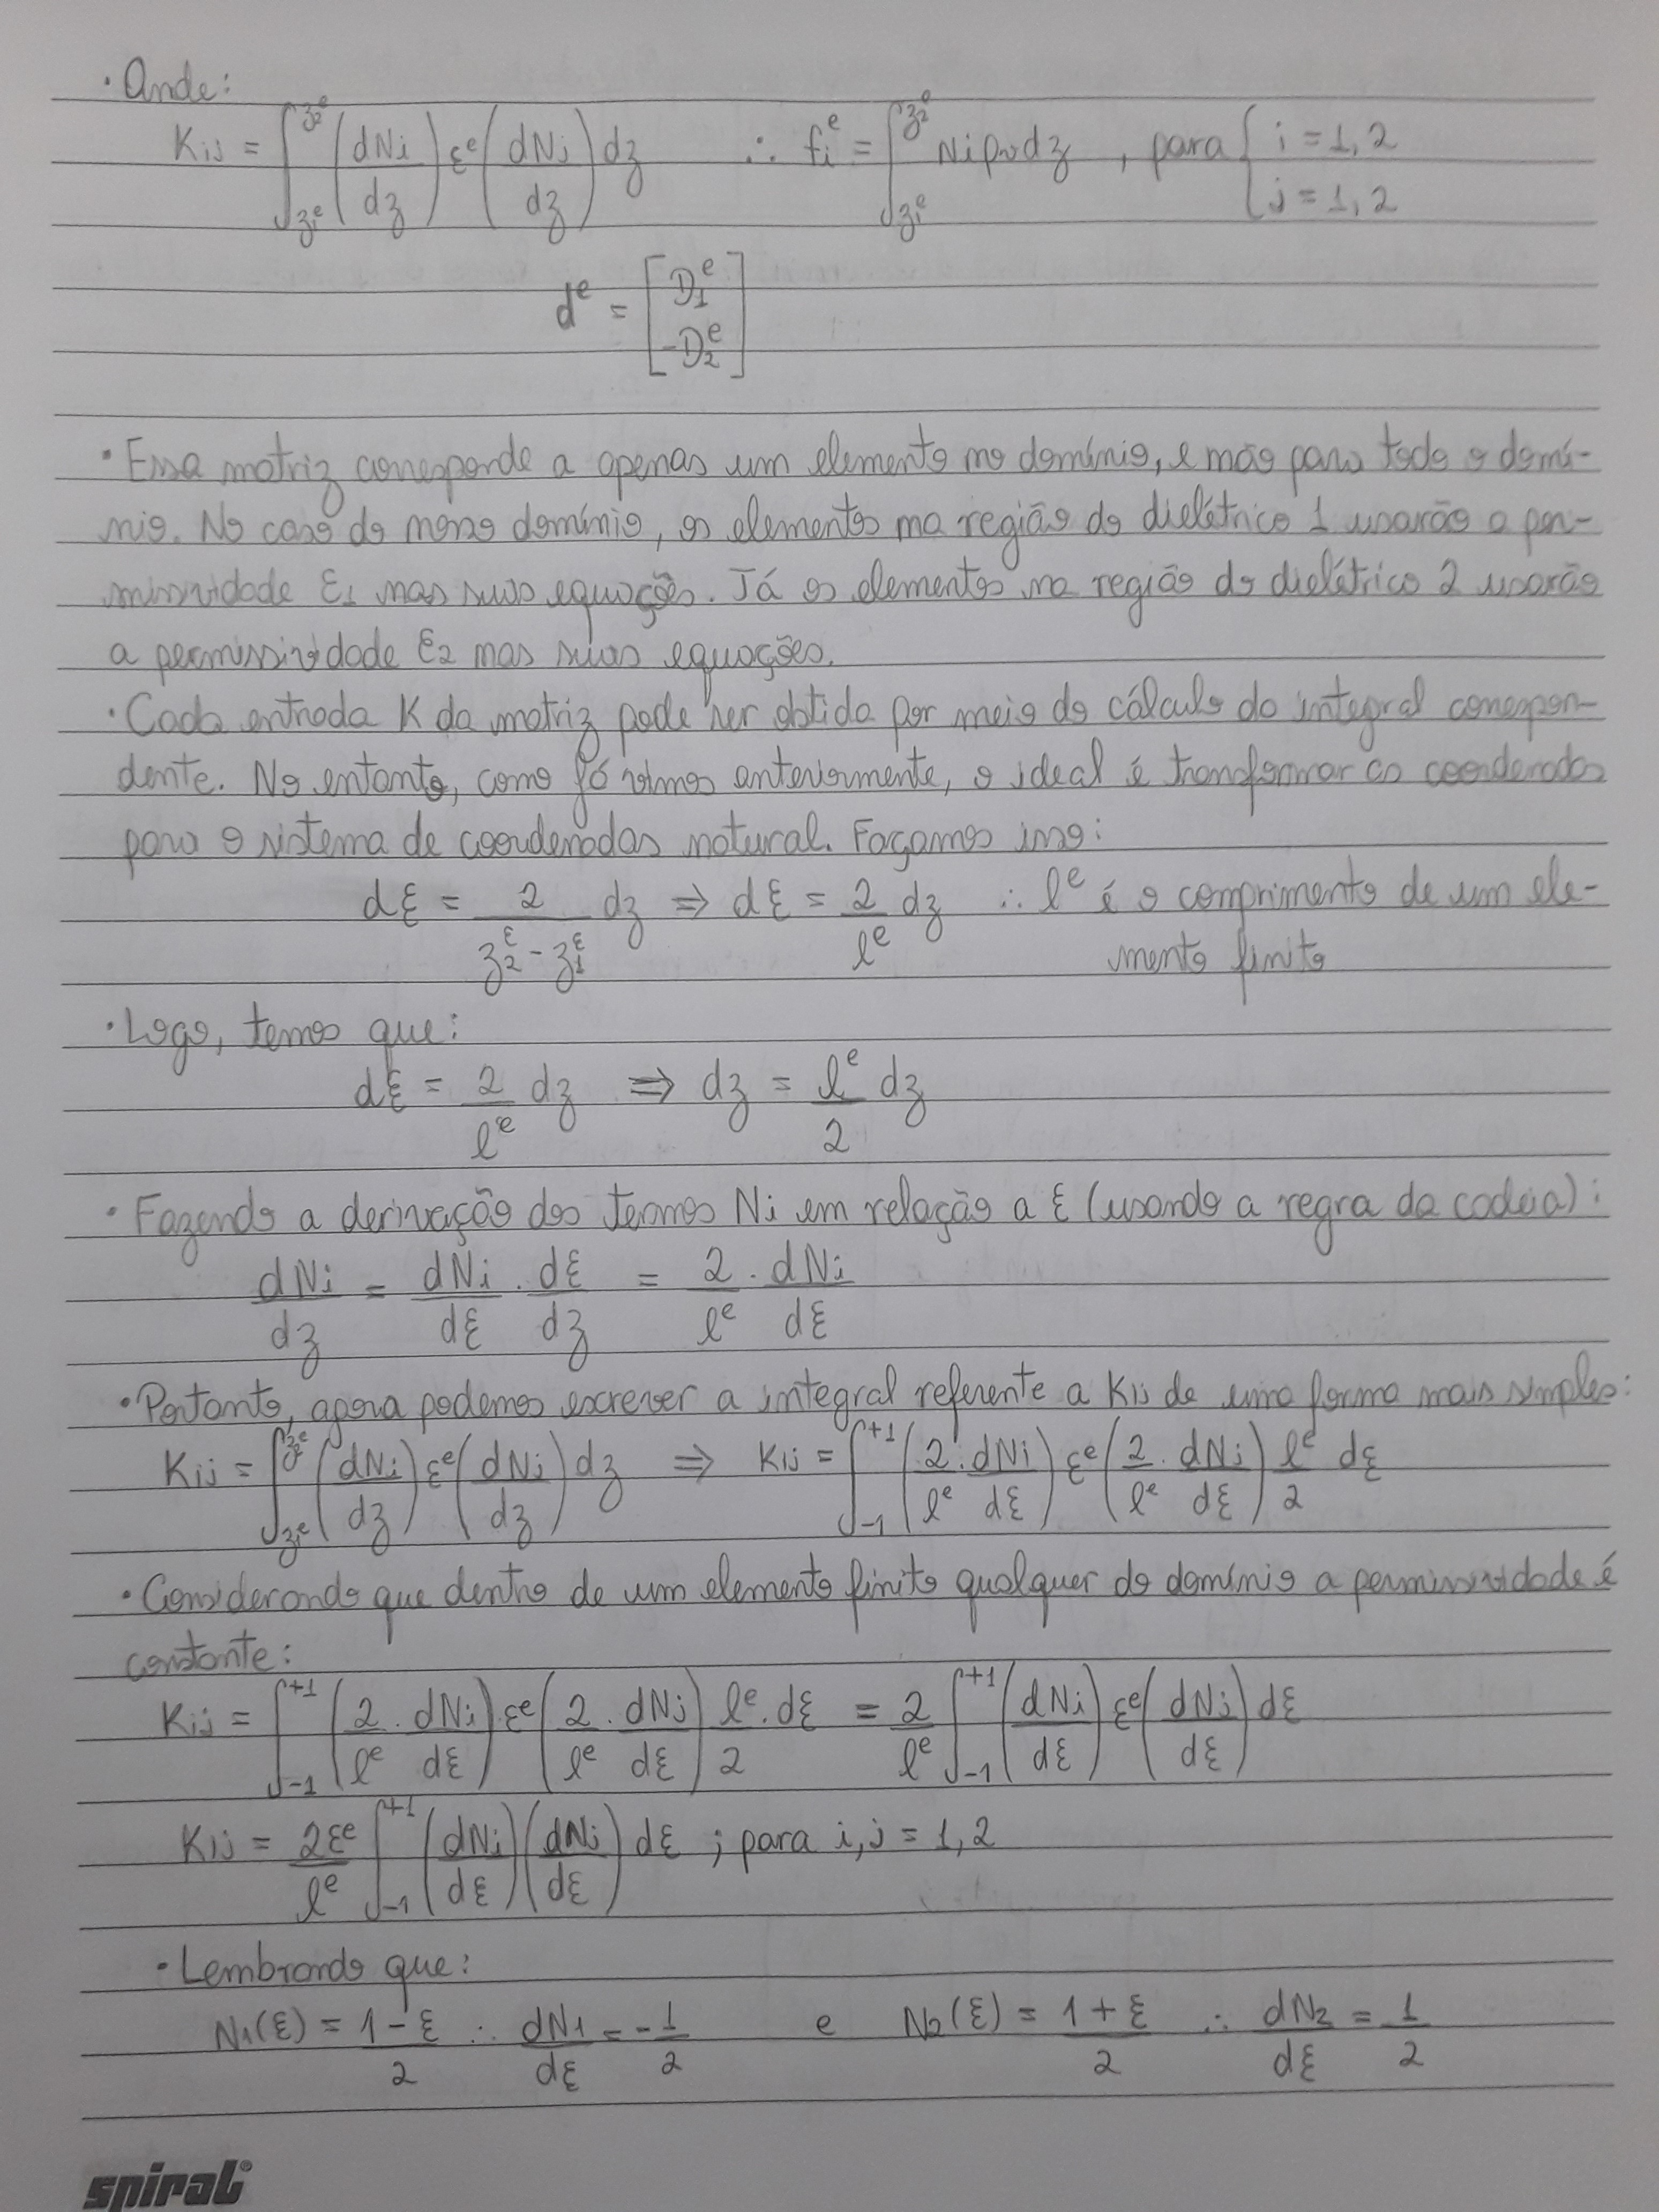
\includegraphics[width=20cm,height=22cm]{Formulação Matemática/Formulacao - Parte 8.jpg}}
    \caption{Formulação - Parte 8}
    \label{fig:fp8}
    \end{figure}
    
    \begin{figure}[!htb]
    \centerline{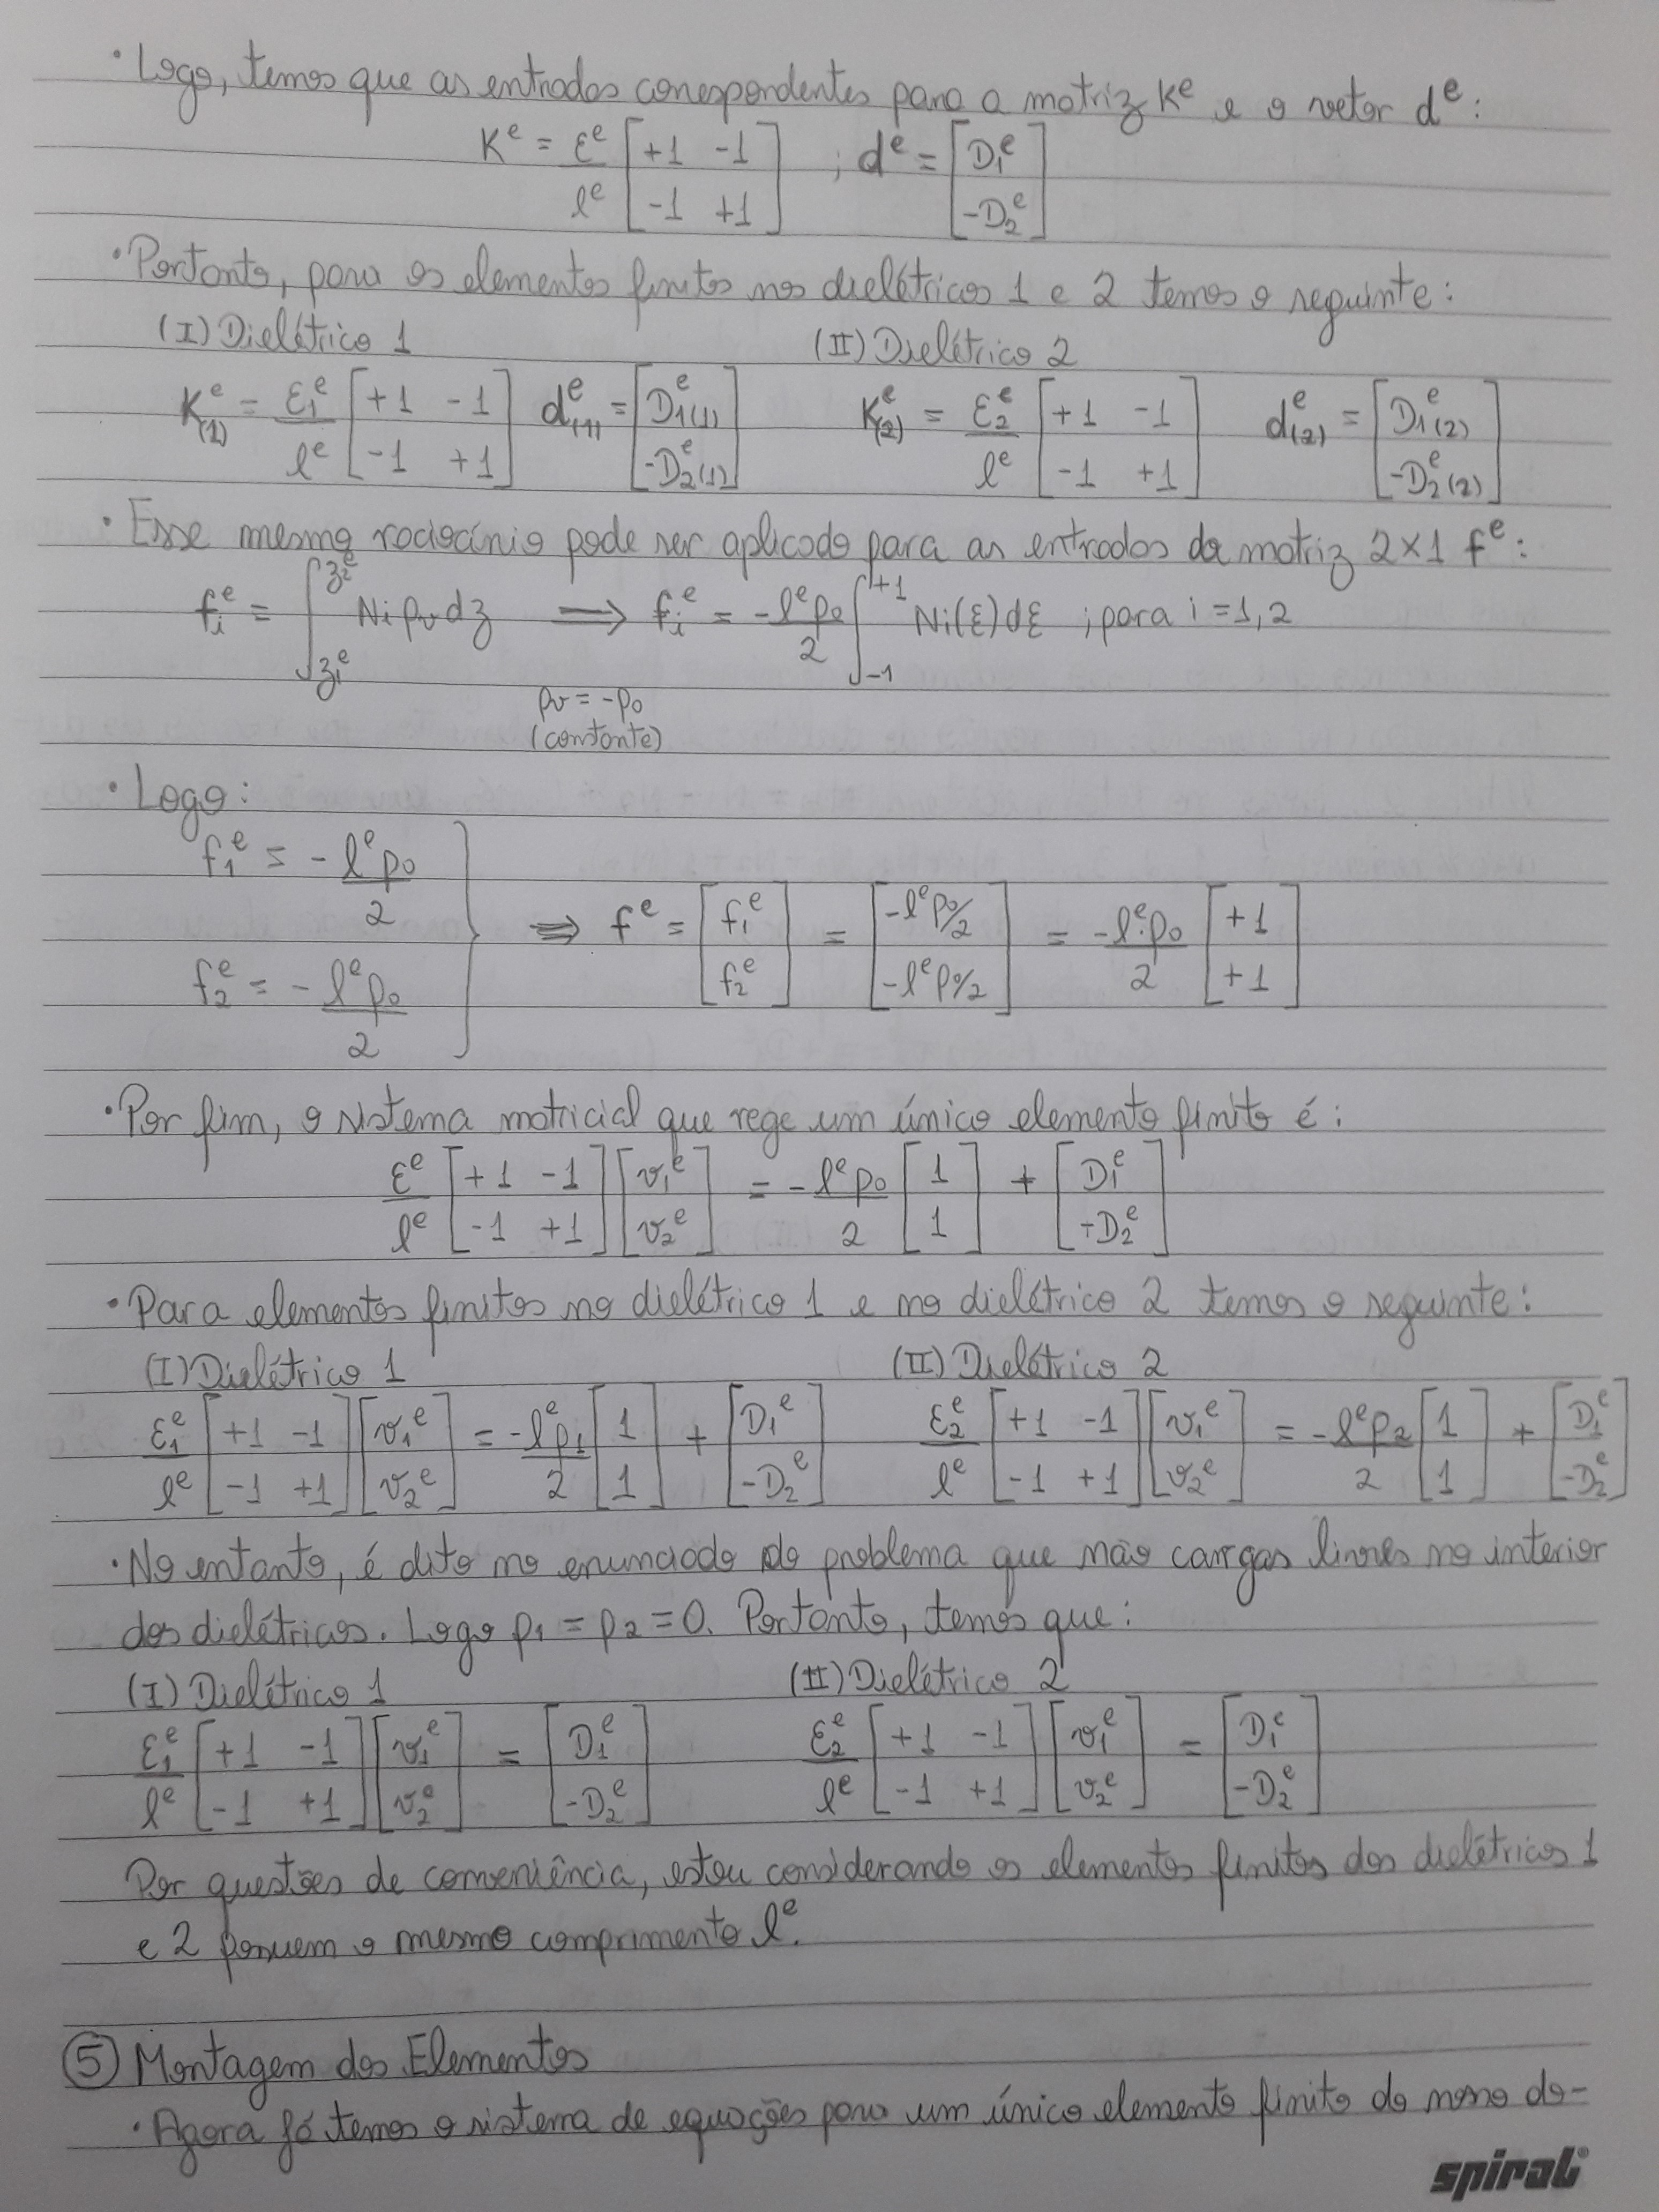
\includegraphics[width=20cm,height=22cm]{Formulação Matemática/Formulacao - Parte 9.jpg}}
    \caption{Formulação - Parte 9}
    \label{fig:fp9}
    \end{figure}
    
    \begin{figure}[!htb]
    \centerline{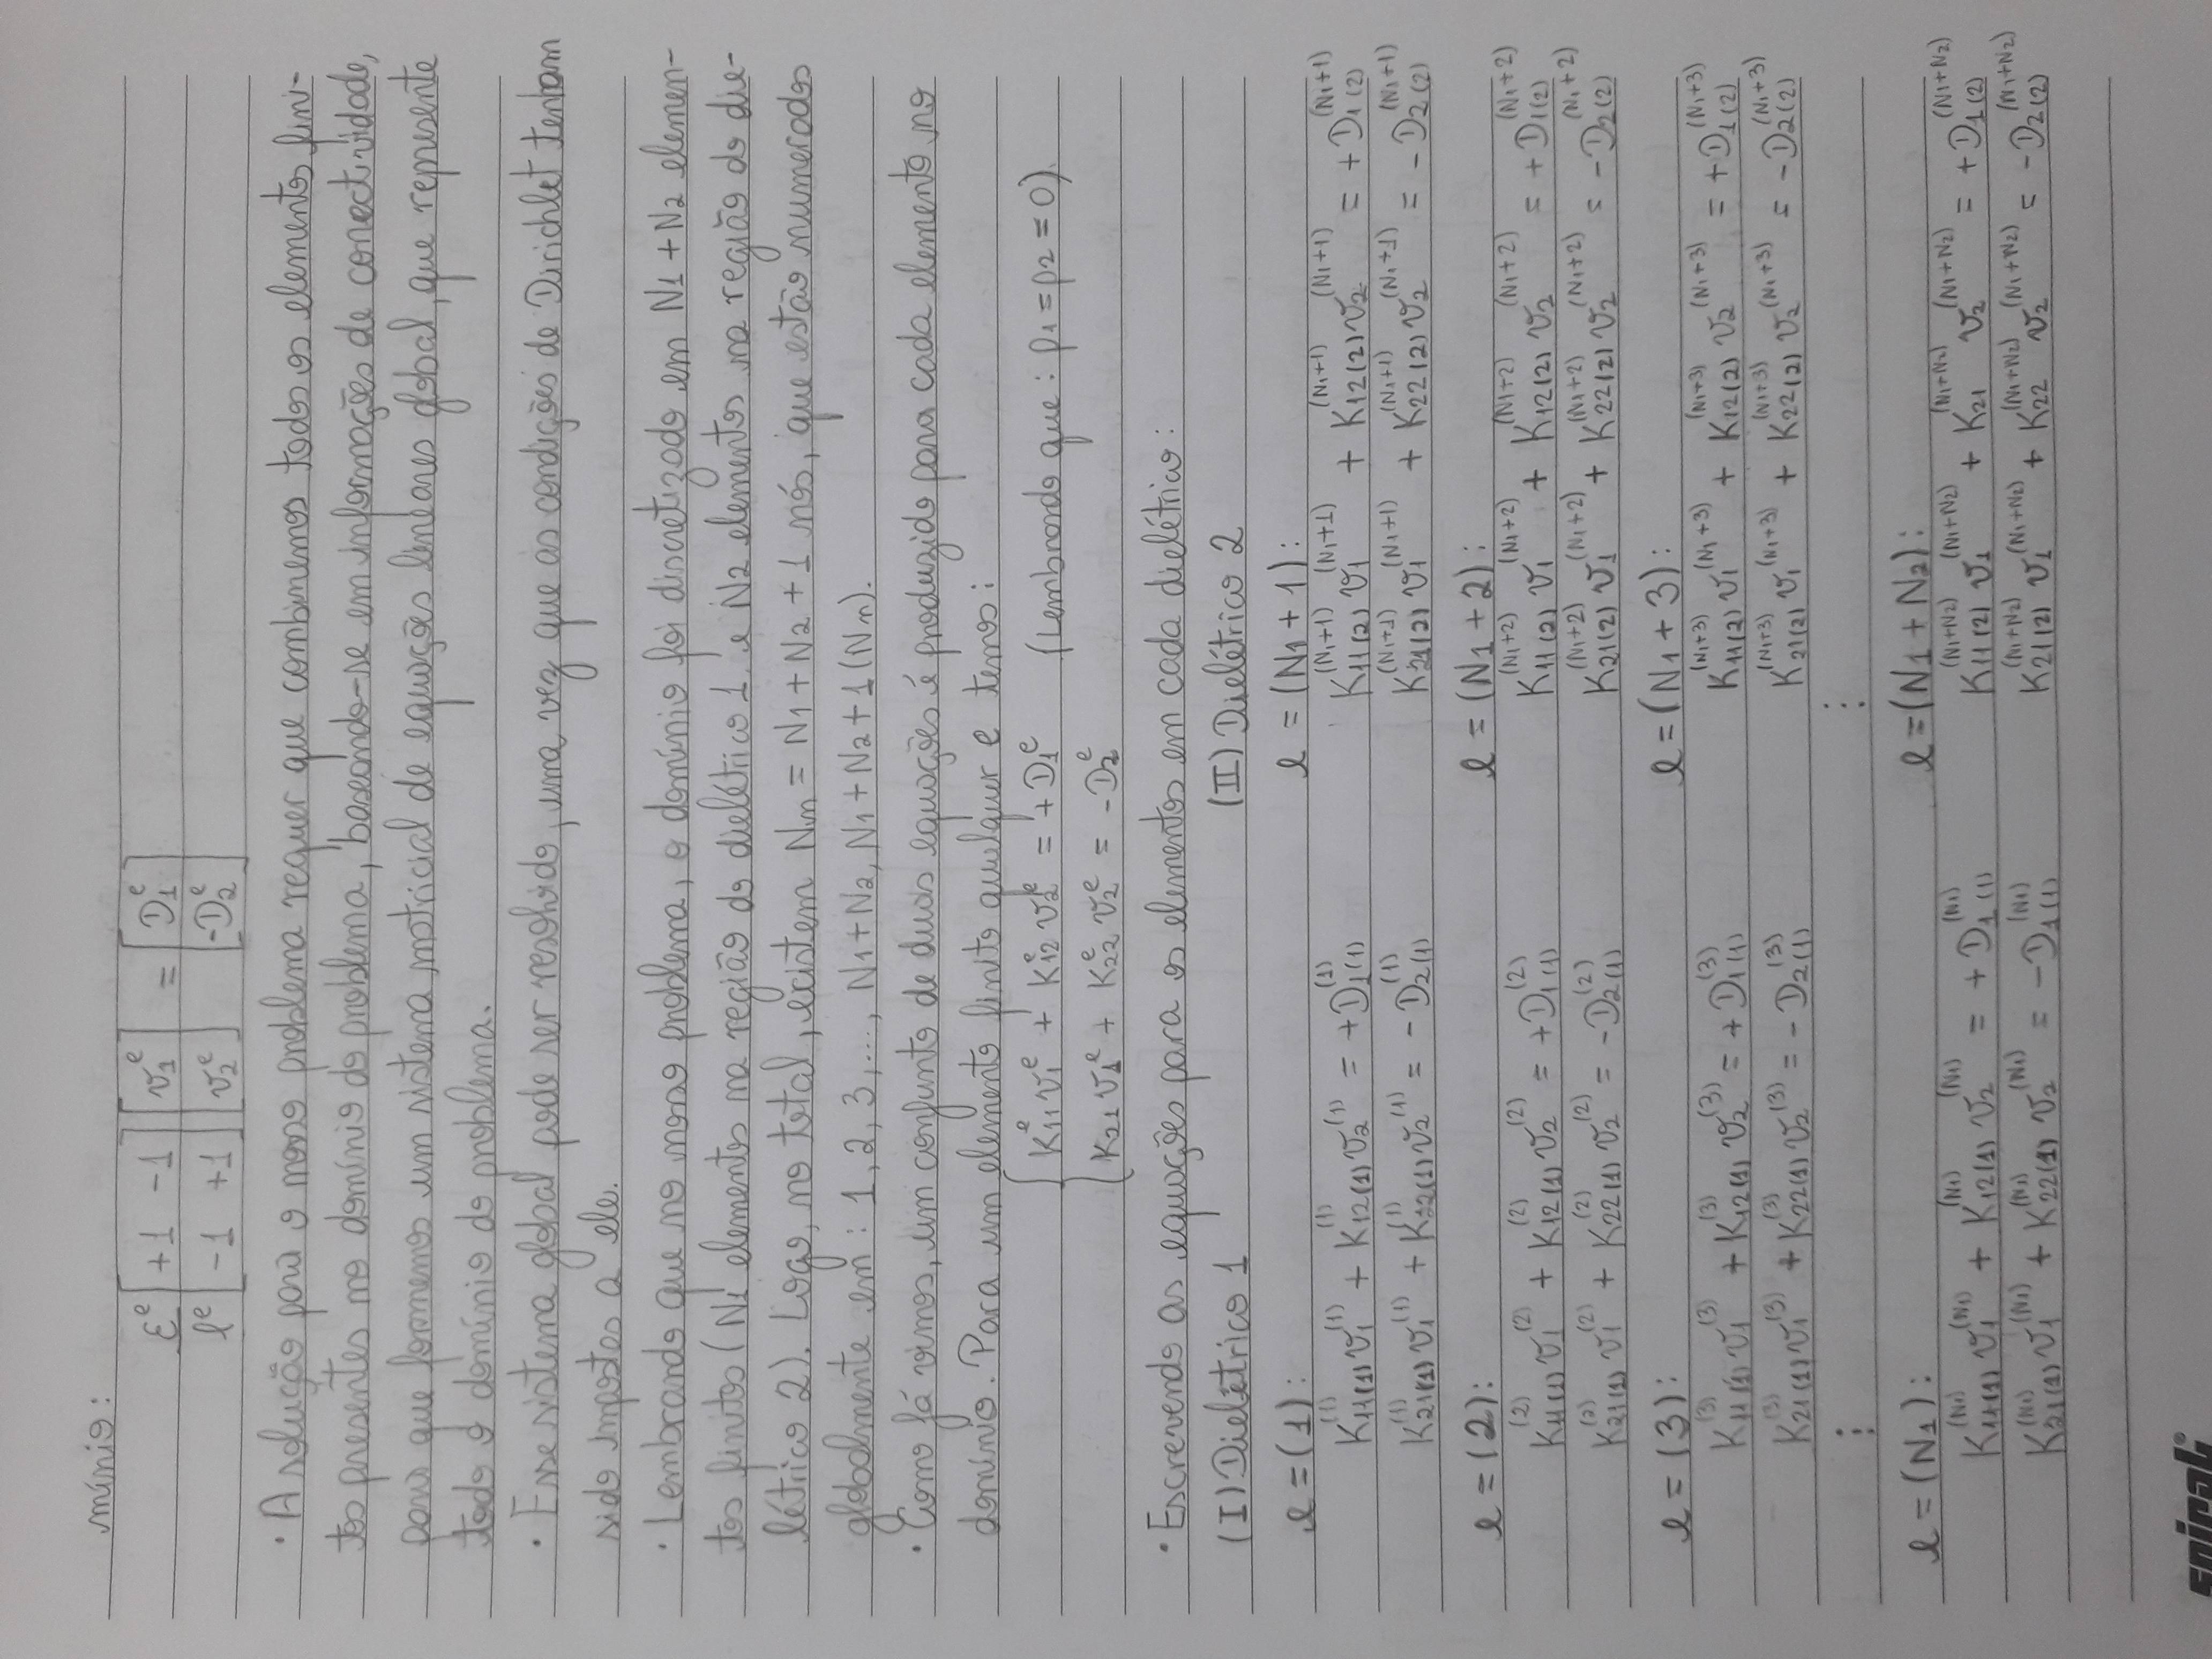
\includegraphics[width=20cm,height=22cm]{Formulação Matemática/Formulacao - Parte 10.jpg}}
    \caption{Formulação - Parte 10}
    \label{fig:fp10}
    \end{figure}
    
    \begin{figure}[!htb]
    \centerline{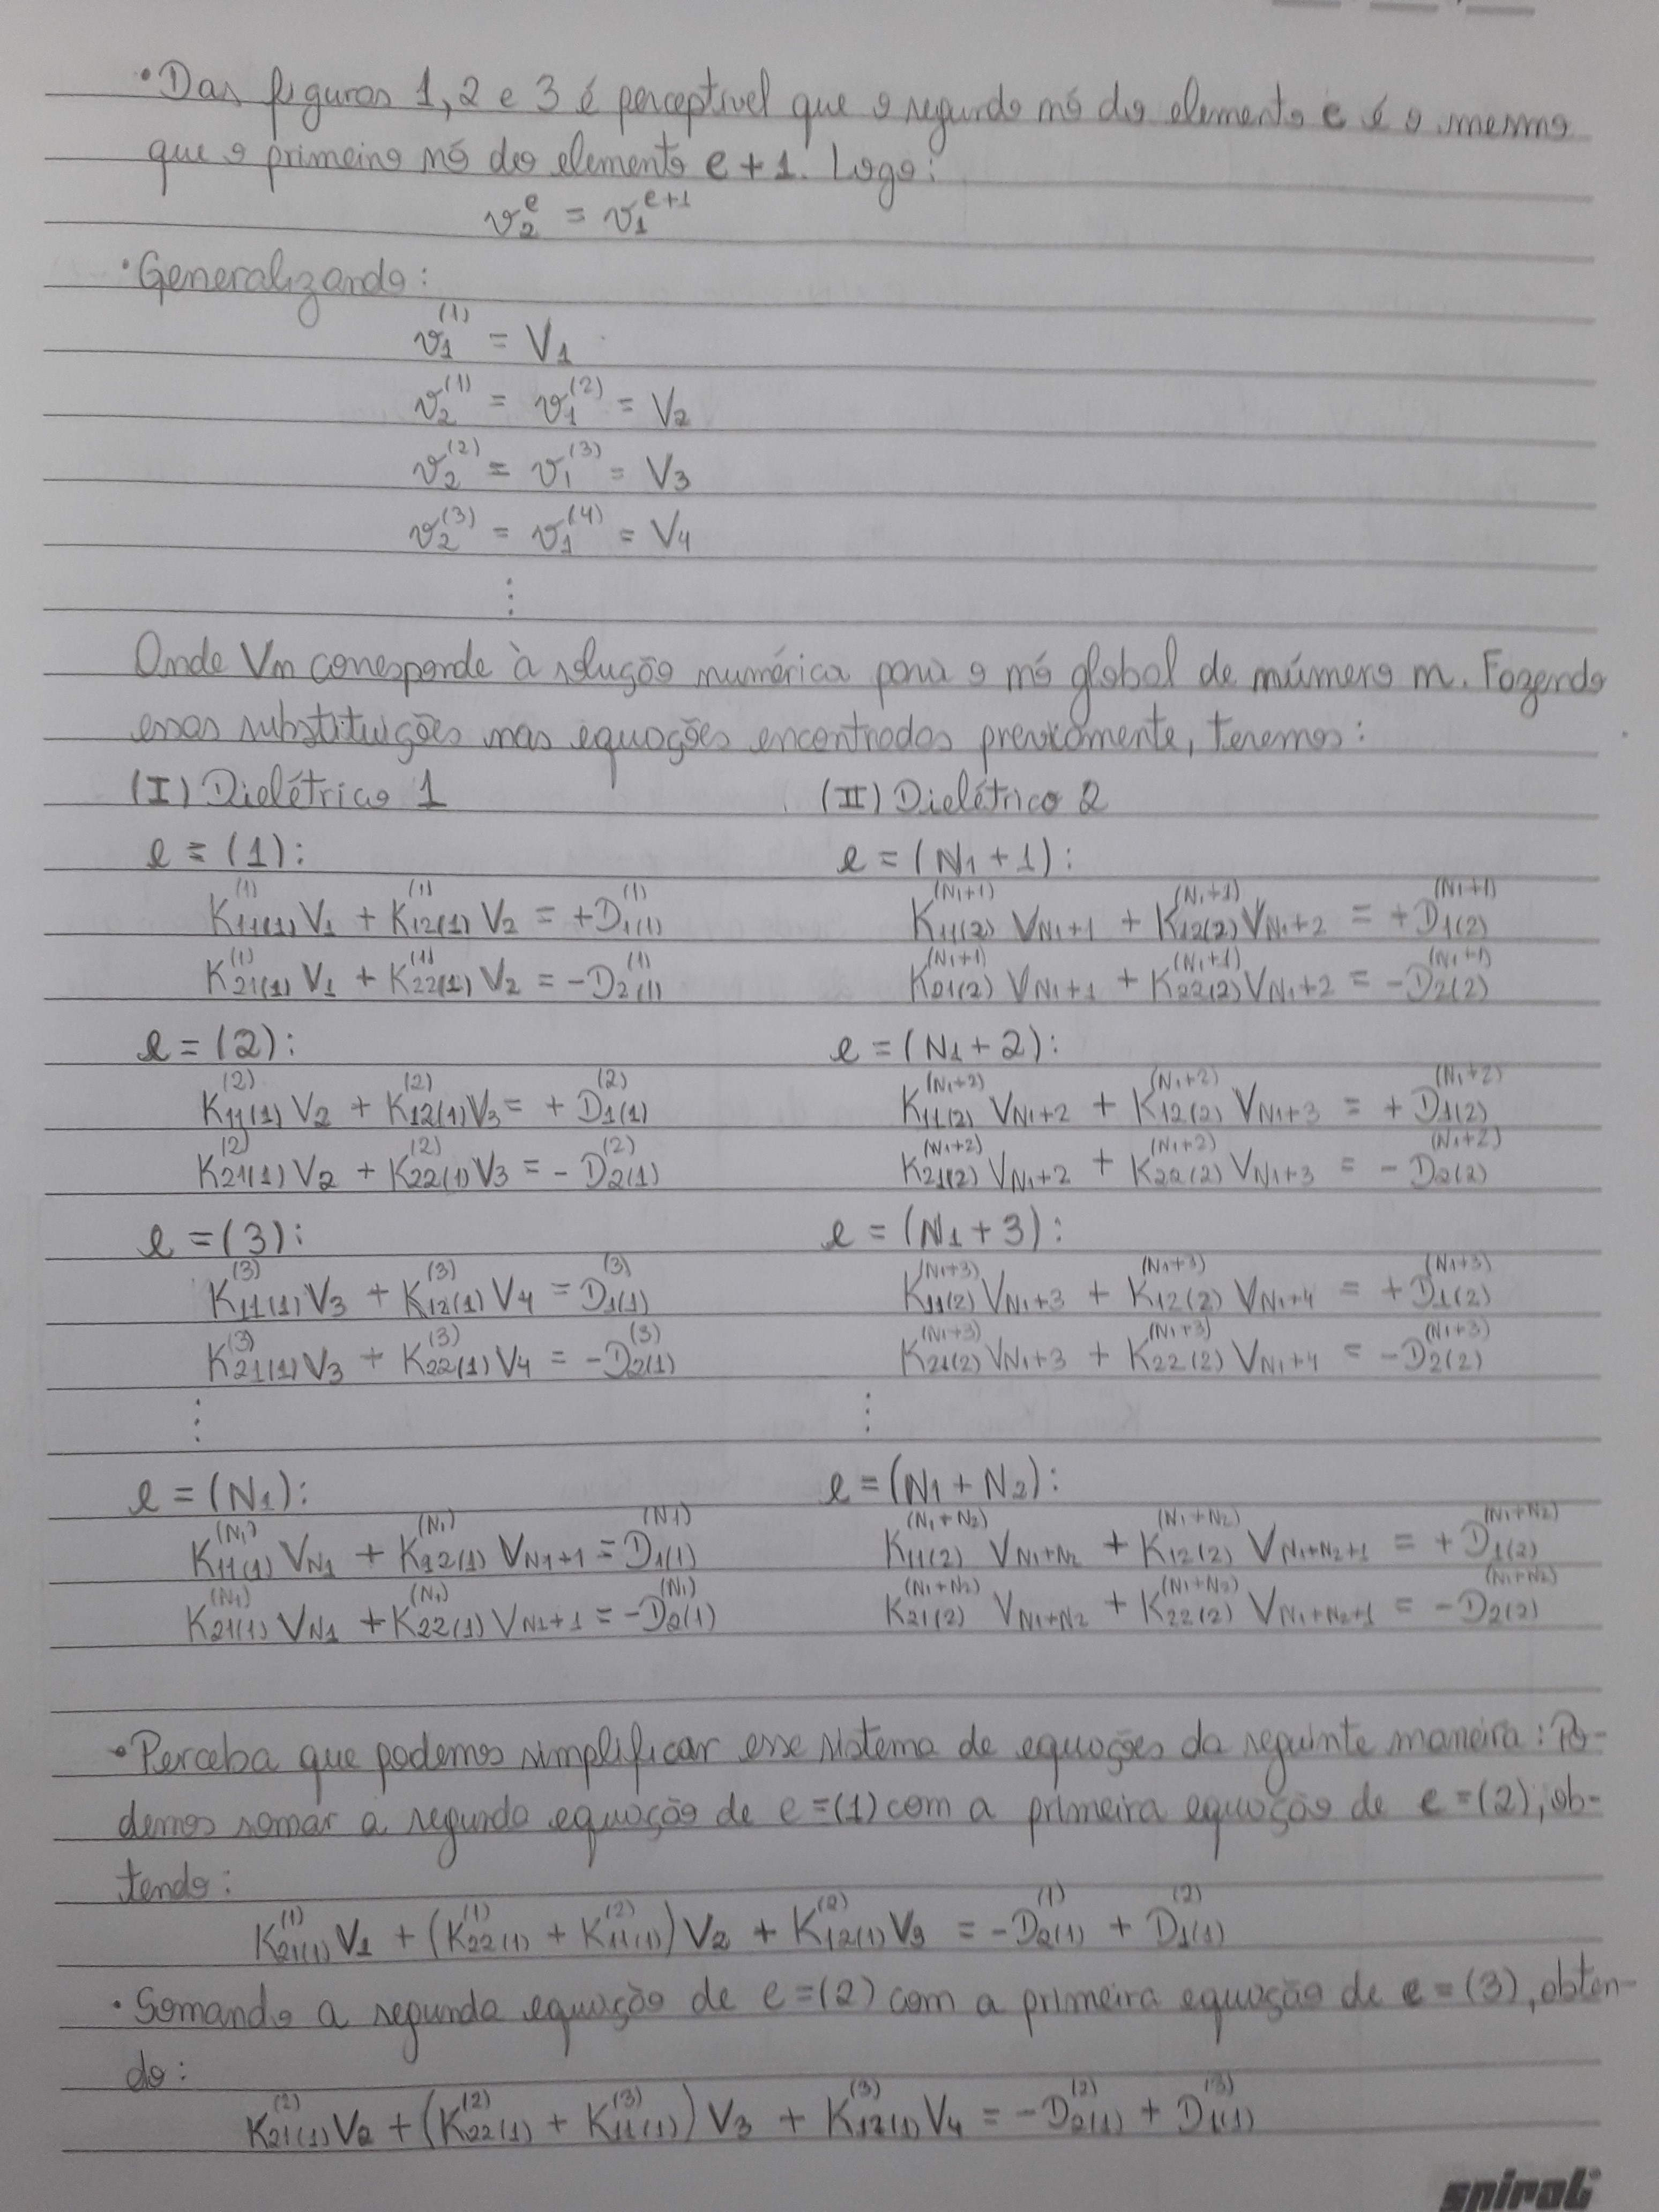
\includegraphics[width=20cm,height=22cm]{Formulação Matemática/Formulacao - Parte 11.jpg}}
    \caption{Formulação - Parte 11}
    \label{fig:fp11}
    \end{figure}
    
    \begin{figure}[!htb]
    \centerline{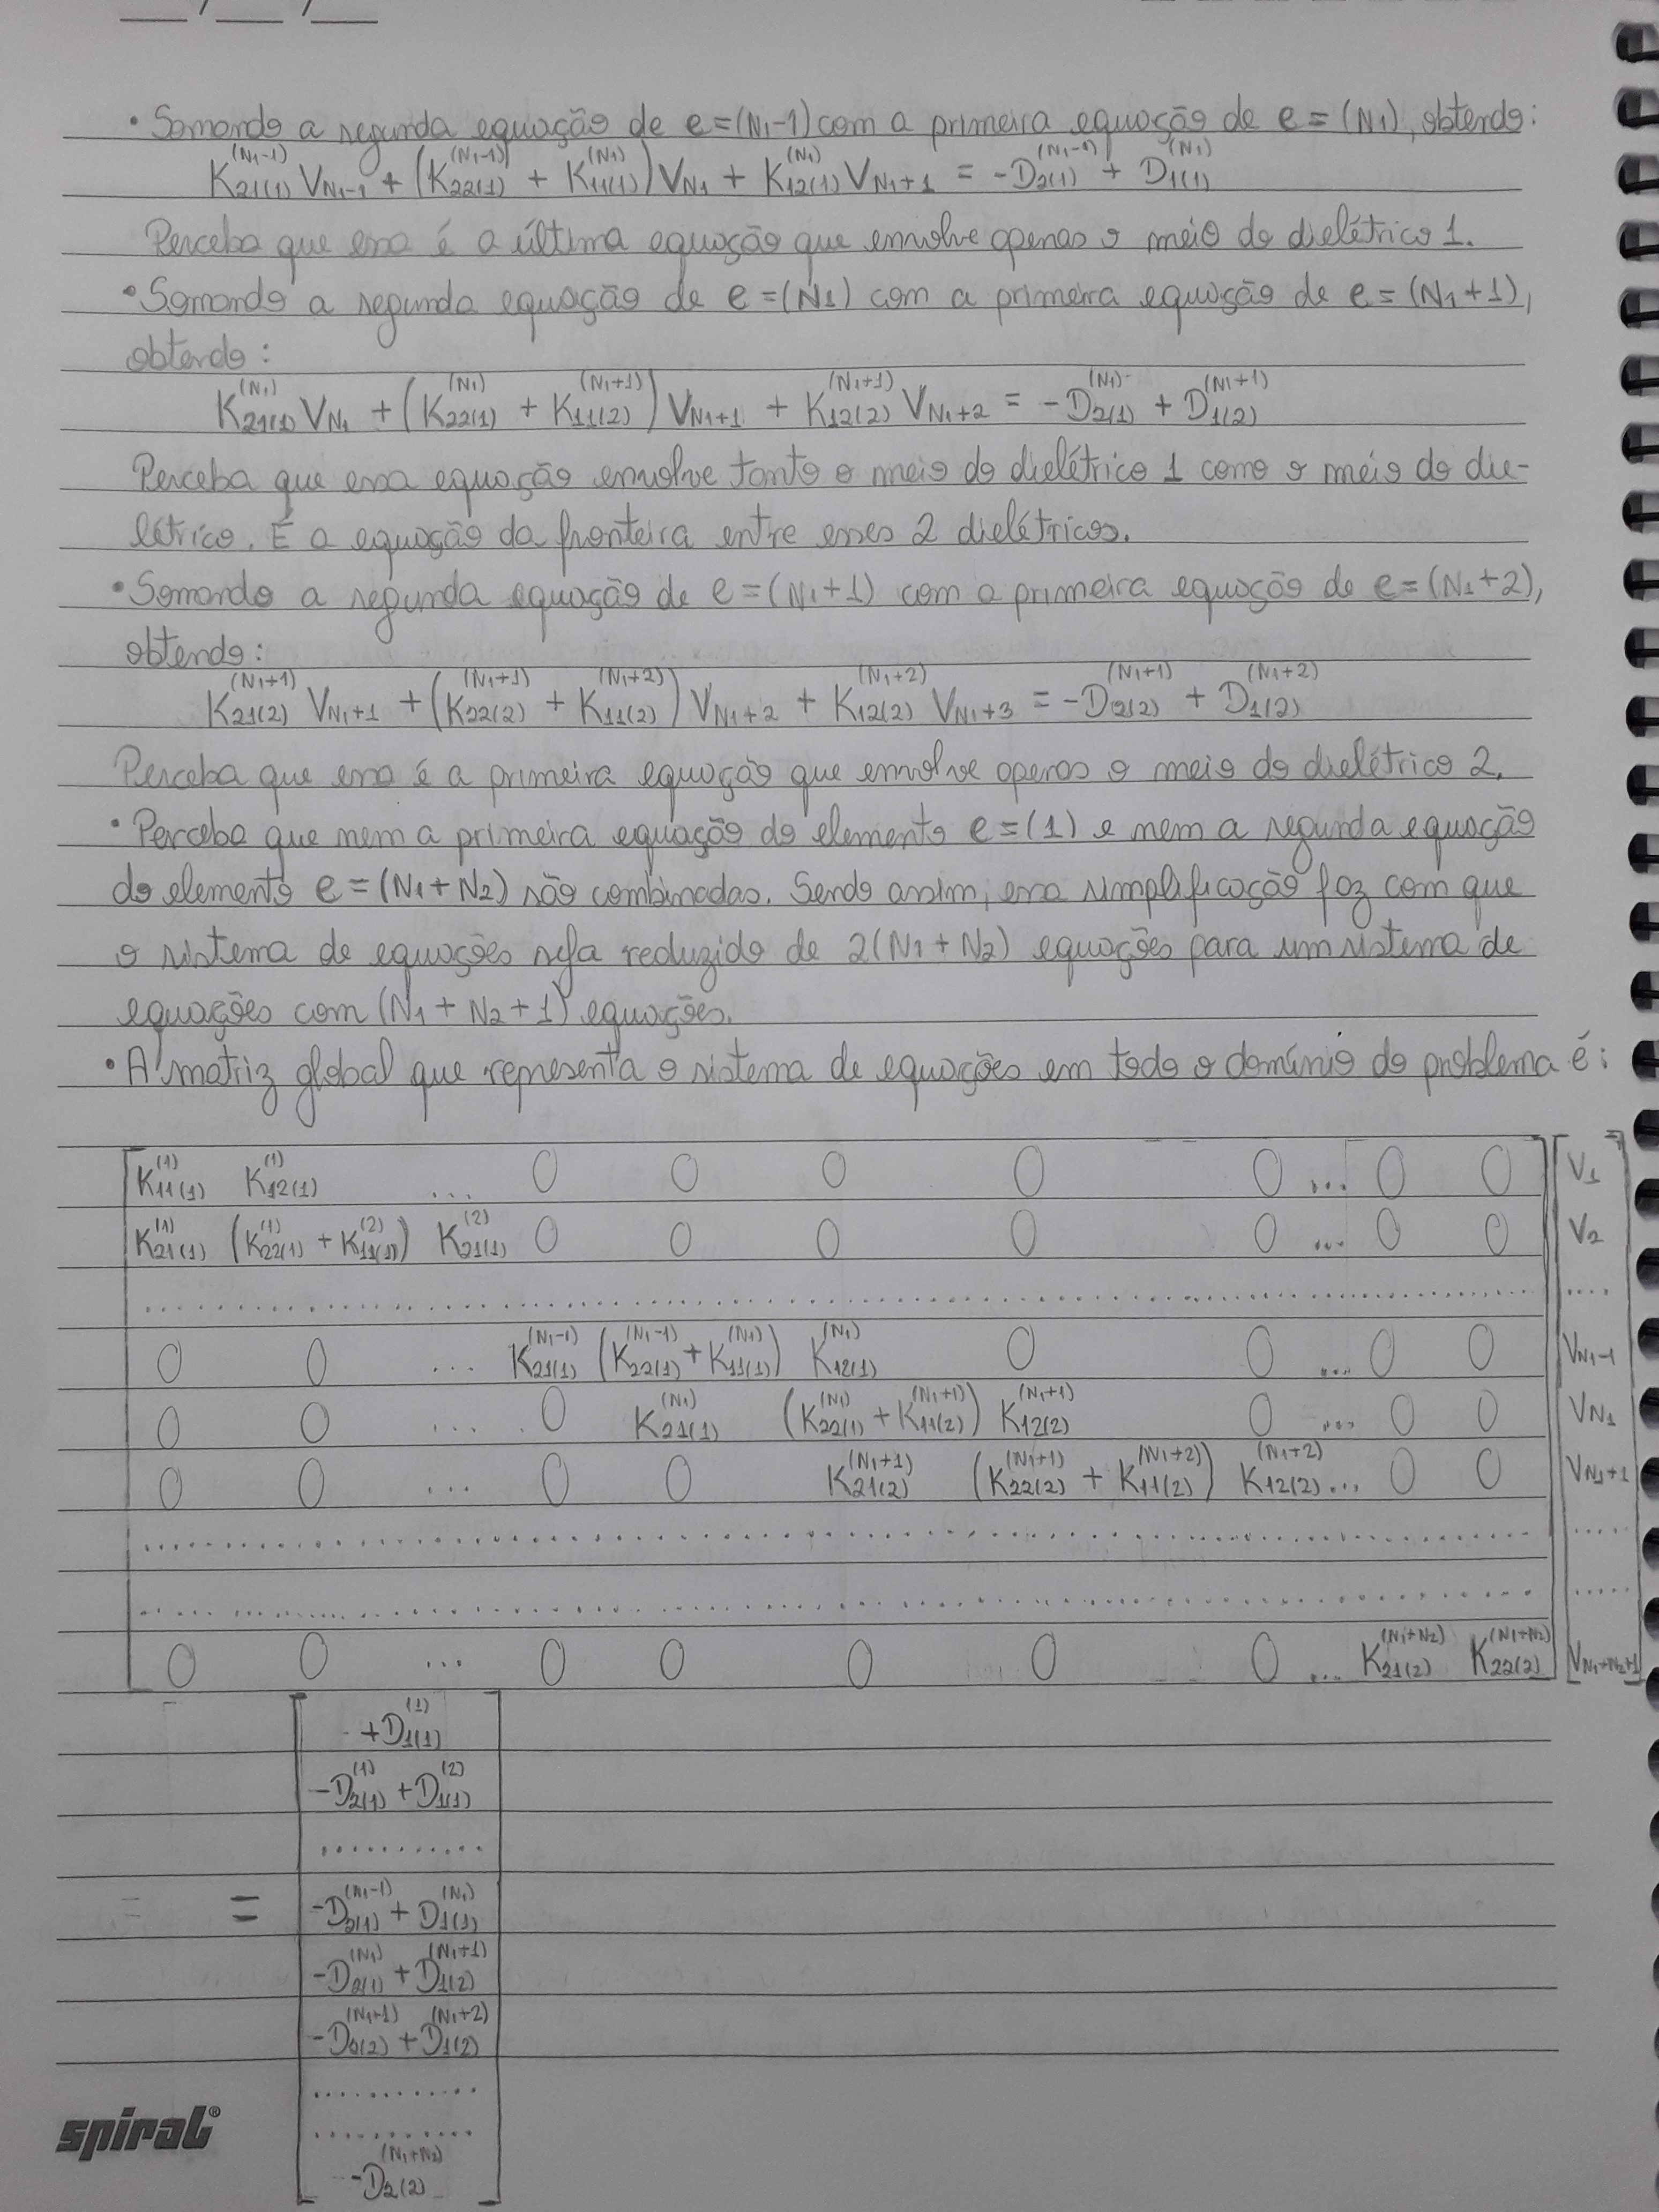
\includegraphics[width=20cm,height=22cm]{Formulação Matemática/Formulacao - Parte 12.jpg}}
    \caption{Formulação - Parte 12}
    \label{fig:fp12}
    \end{figure}
    
    \begin{figure}[!htb]
    \centerline{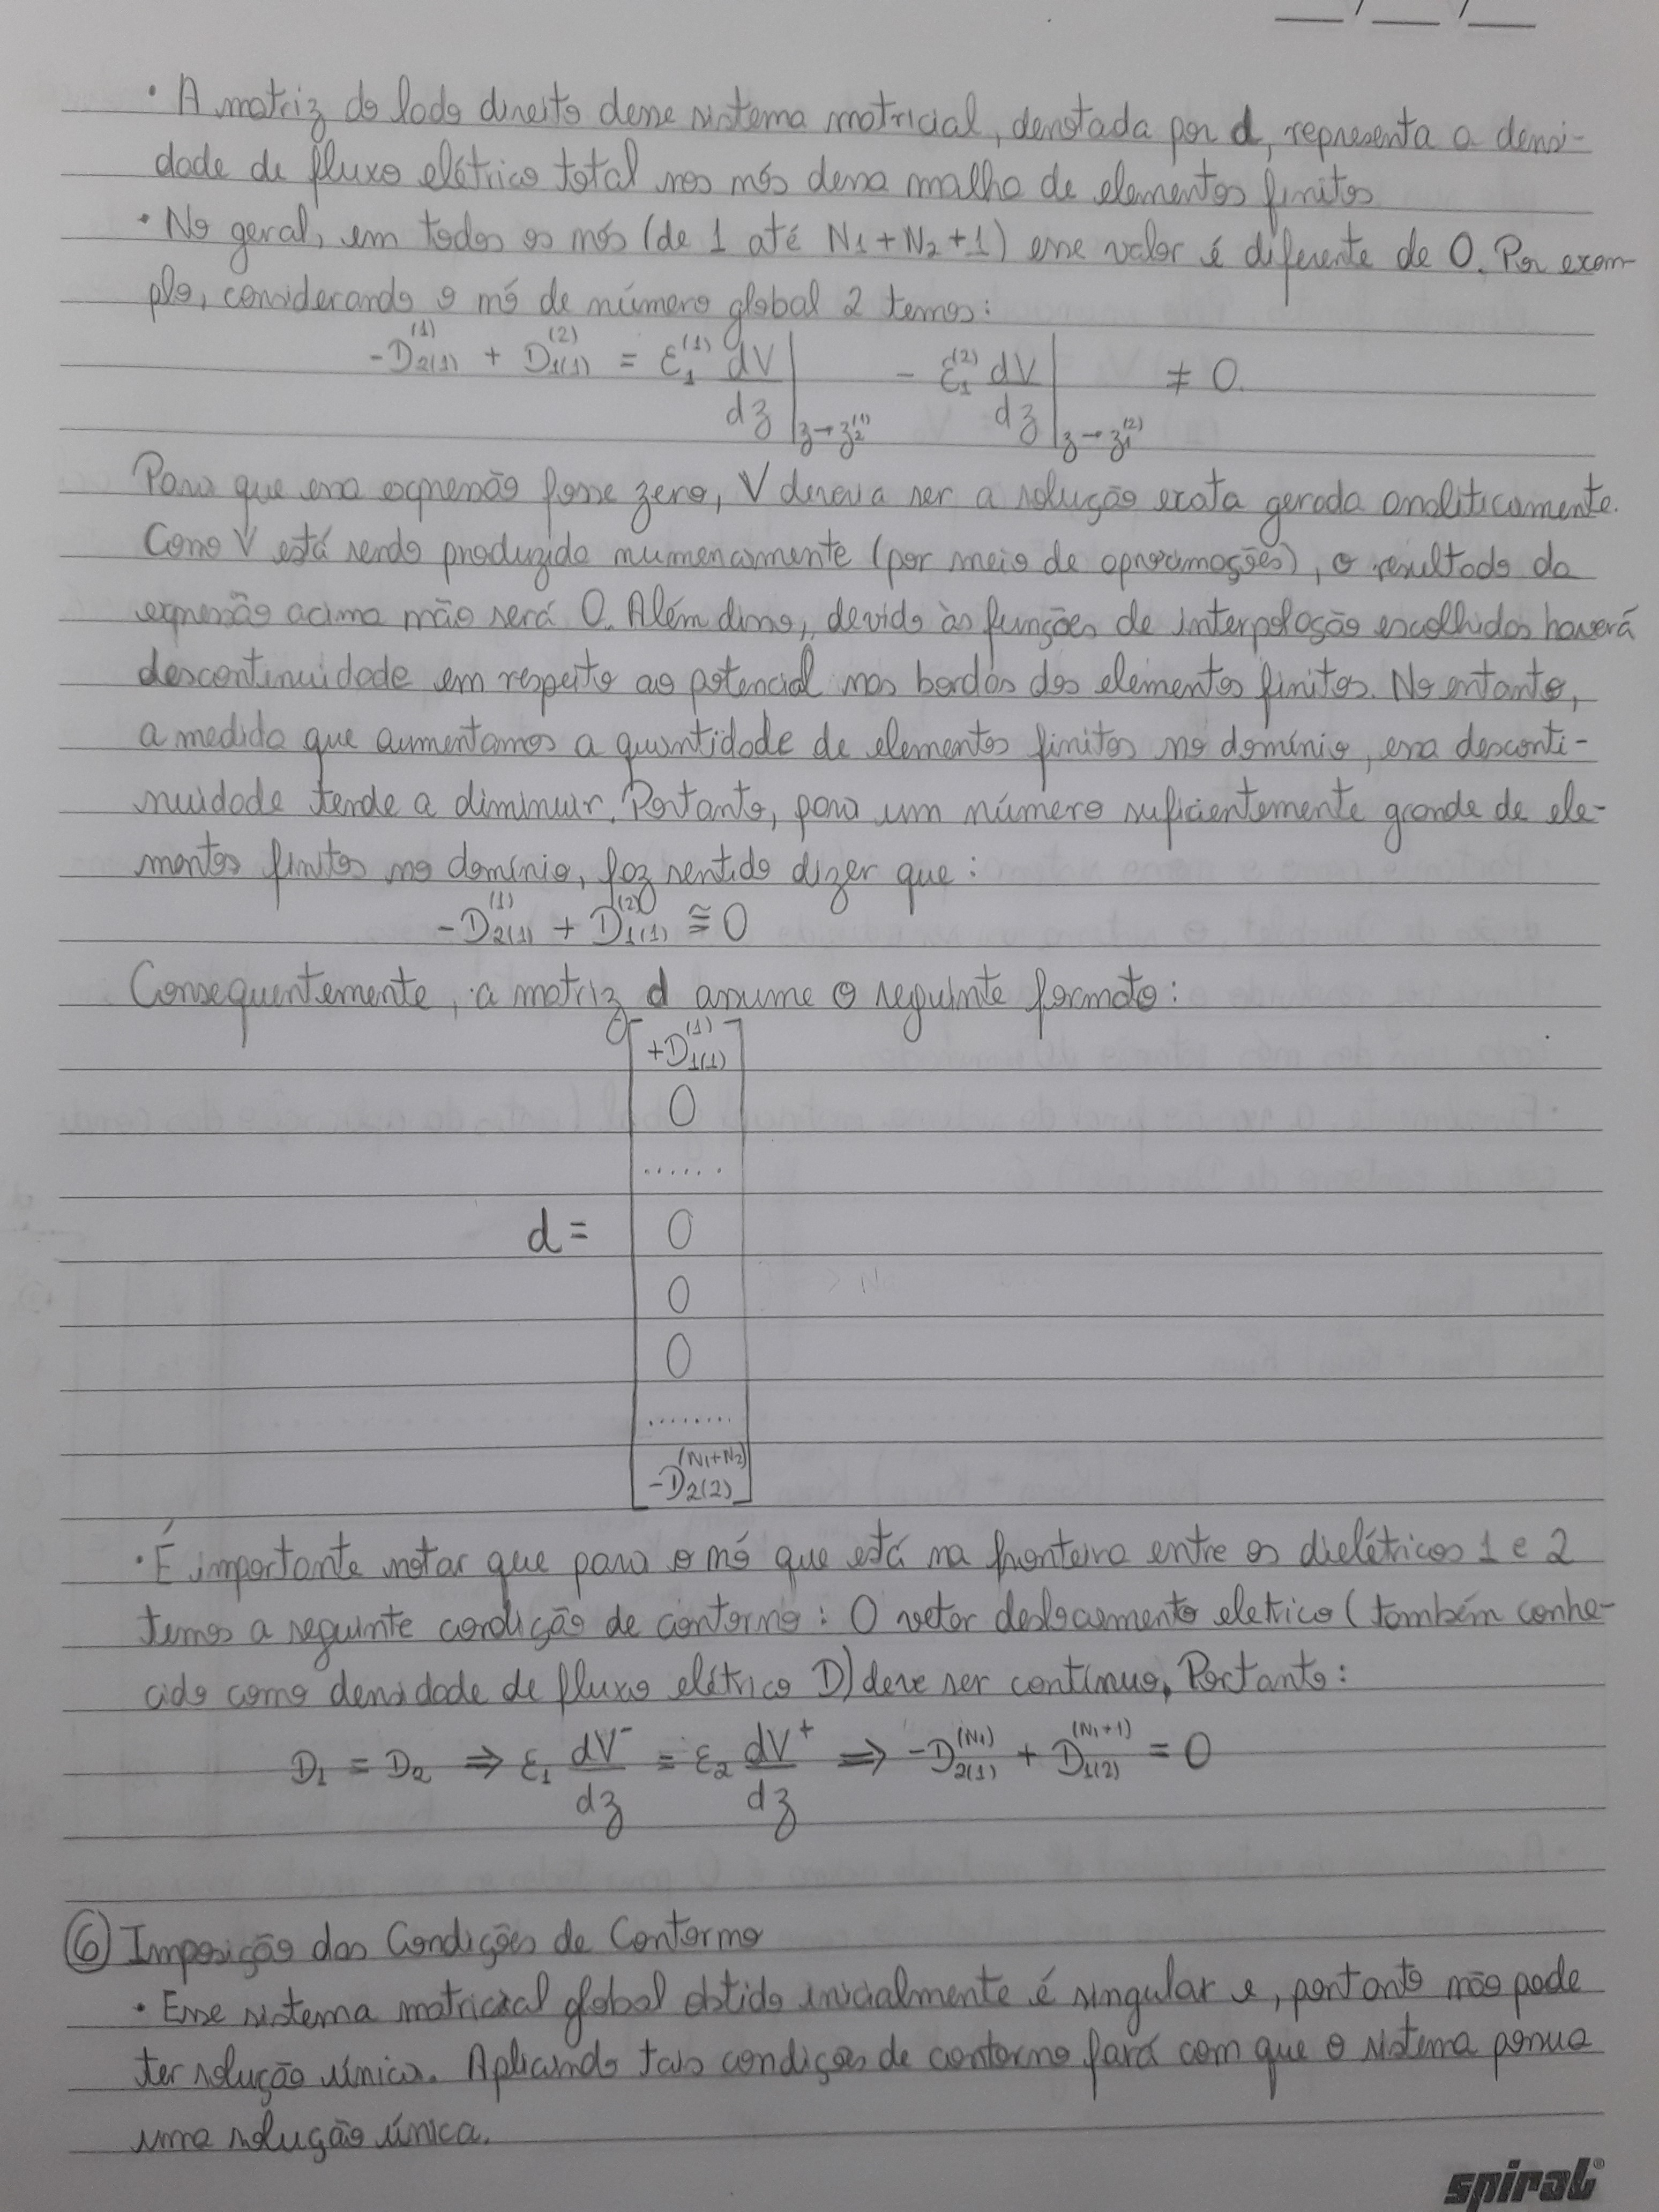
\includegraphics[width=20cm,height=22cm]{Formulação Matemática/Formulacao - Parte 13.jpg}}
    \caption{Formulação - Parte 13}
    \label{fig:fp13}
    \end{figure}
    
    \begin{figure}[!htb]
    \centerline{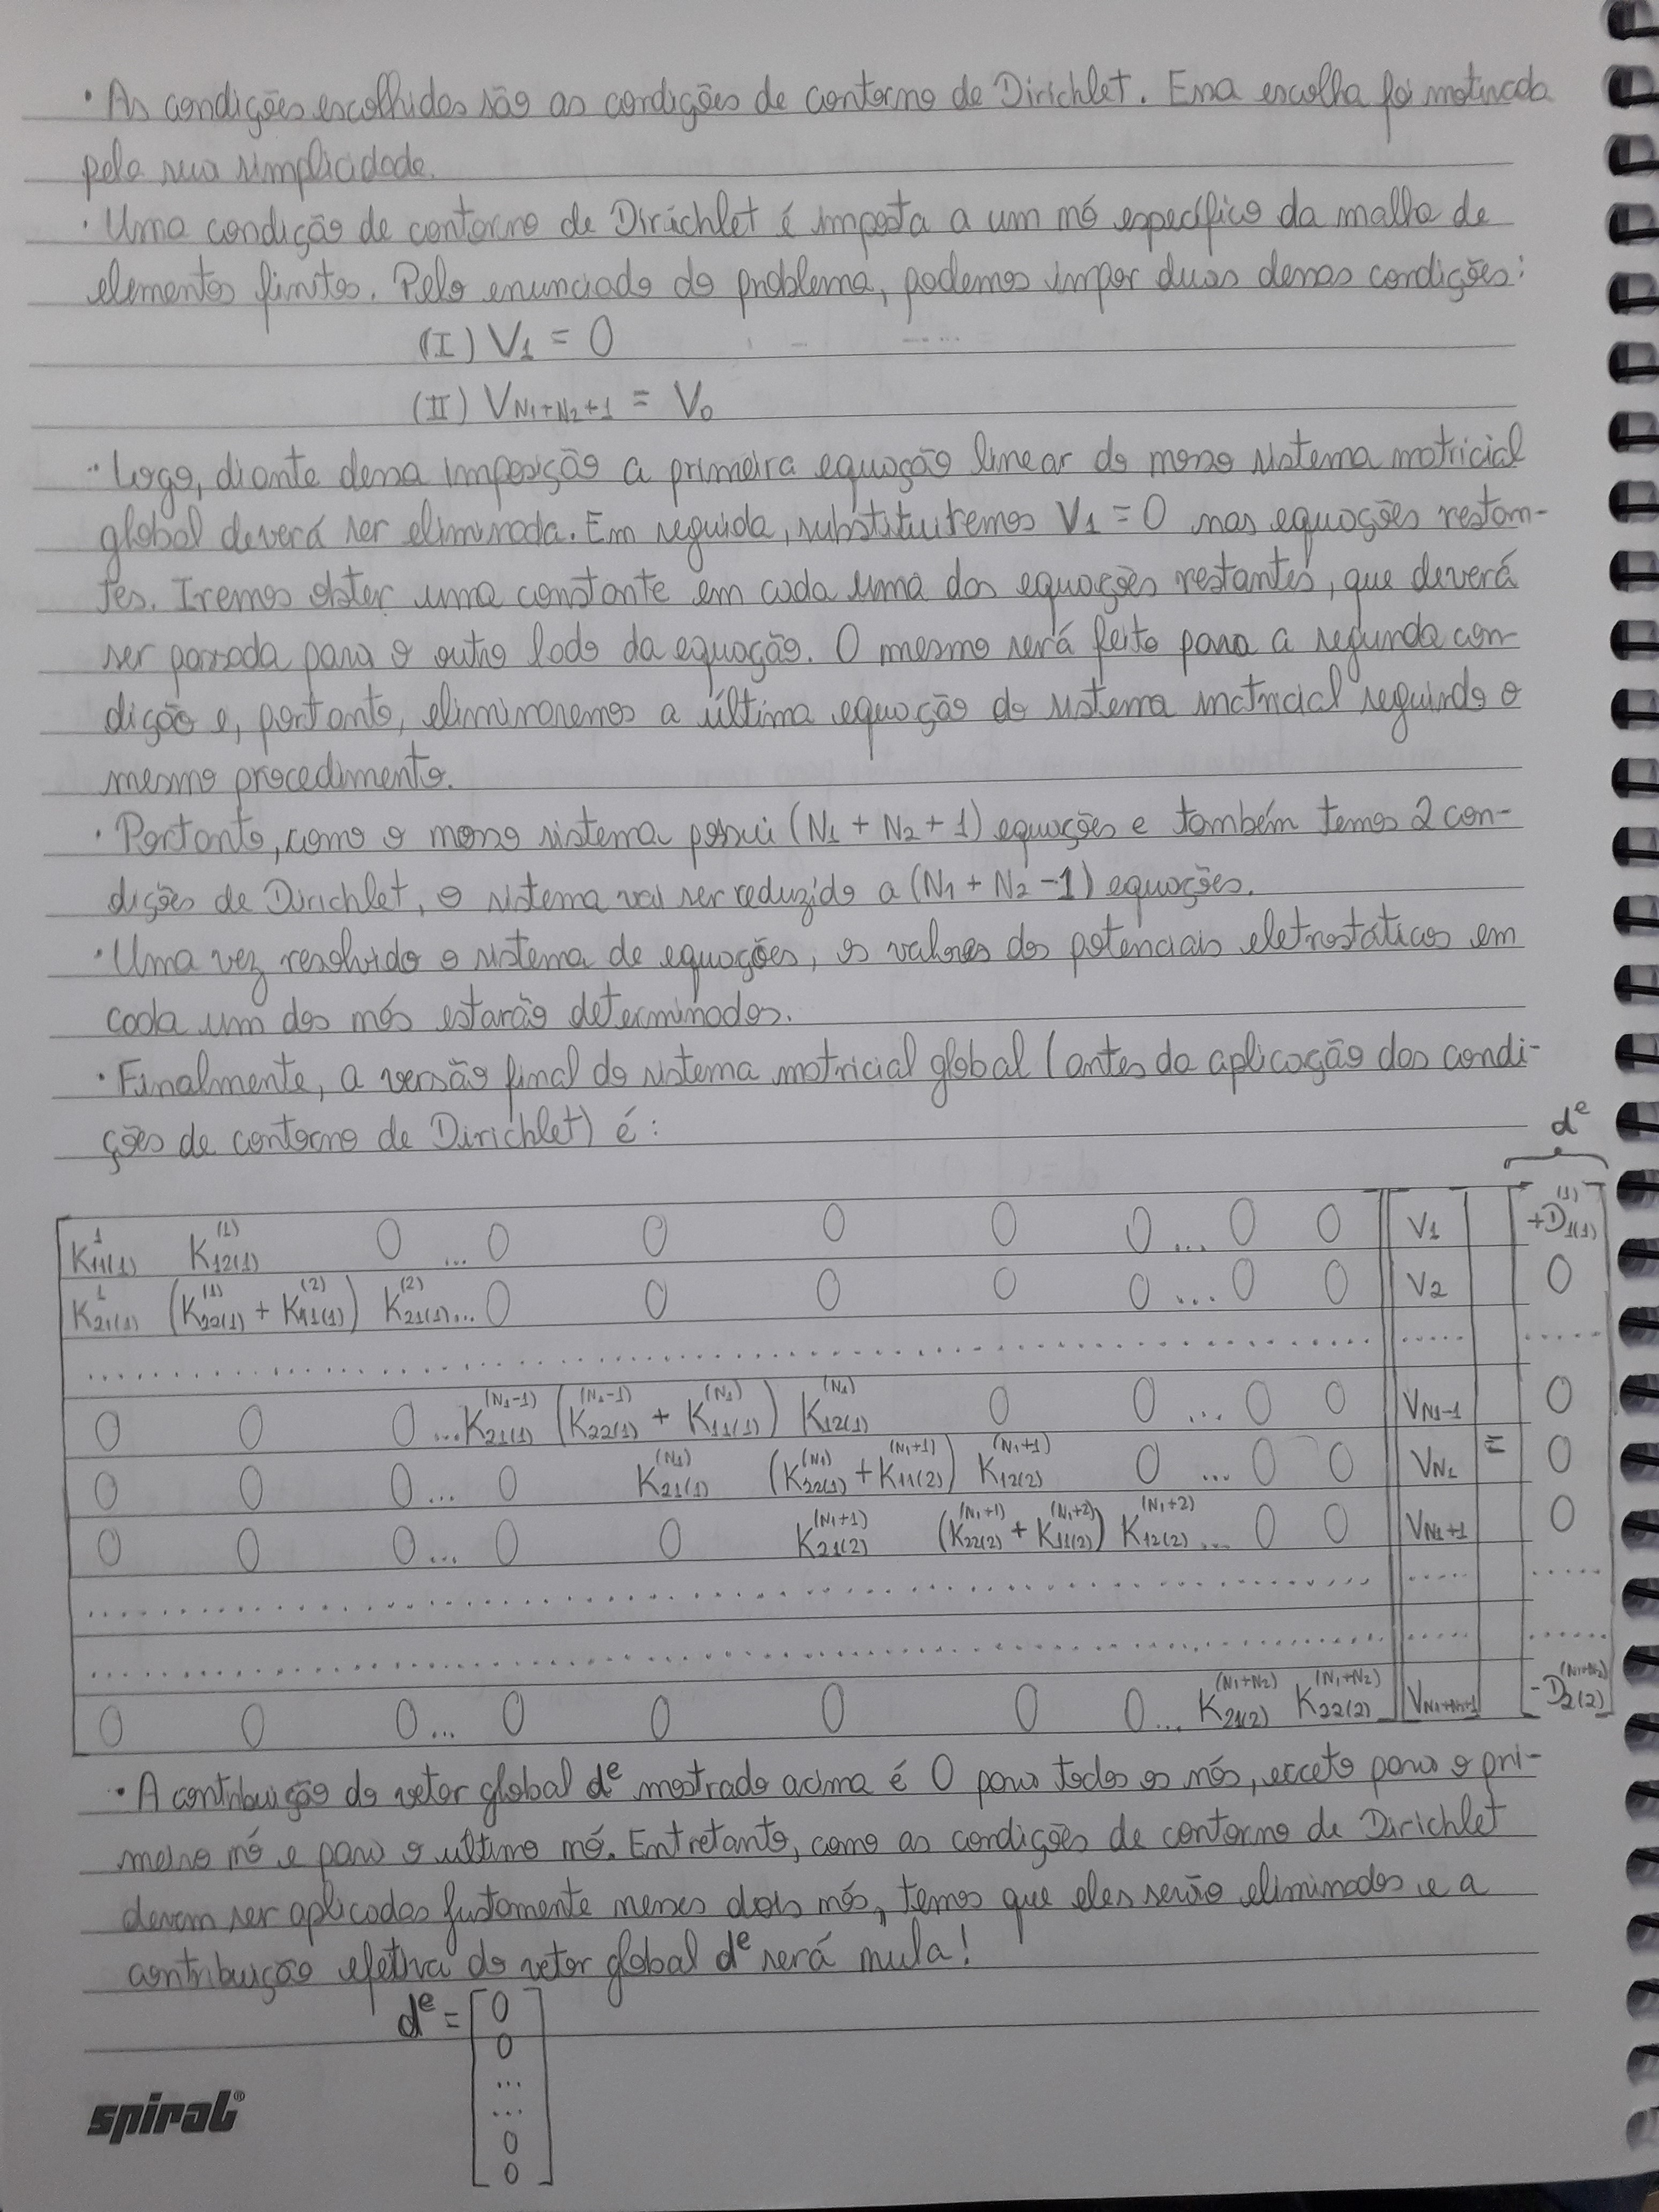
\includegraphics[width=20cm,height=22cm]{Formulação Matemática/Formulacao - Parte 14.jpg}}
    \caption{Formulação - Parte 14}
    \label{fig:fp14}
    \end{figure}
    

\section{Implementação do métodos dos elementos finitos 1D}
    
    \subsection{Implementação}
    \begin{itemize}
    \item Para a implementação computacional do método dos elementos finitos 1D, optou-se pela utilização da linguagem Python devido a sua simplicidade e abundância de bibliotecas voltadas para o trabalho com matrizes e vetores, sendo assim bastante conveniente para o problema apresentado.
    \item As bibliotecas em questão utilizadas foram: \textbf{numpy} (para trabalhar com matrizes, vetores e sistemas lineares) e \textbf{matplotlib} (para trabalhar com a representação gráfica dos resultados obtidos).
    \end{itemize}
    
    \subsection{Funcionamento}
    \begin{itemize}
    \item Ao ser executado, o programa receberá como entrada os seguintes dados necessários para a resolução do problema:
        \begin{itemize}
        \item A medida do lado L das placas capacitor (cm).
        \item O potencial eletrostático Vo na placa superior do capacitor (V).
        \item A constante dielétrica do dielétrico 1, $\epsilon_{r1}$.
        \item A constante dielétrica do dielétrico 2, $\epsilon_{r2}$.
        \item A quantidade de elementos finitos no meio do dielétrico 1, $n_{1}$, e a quantidade de elementos finitos no meio do dielétrico 2, $n_{2}$.
        \item O comprimento do dielétrico 1, $d_{1}$, e o comprimento do dielétrico 2, $d_{2}$ (mm).
        \end{itemize}
    \item Após isso, ele converterá a medida do lado do capacitor e as medidas do comprimento dos dielétricos 1 e 2 para a unidade metro (m), conforme o SI.
    \item Além disso, o programa calculará a distância total d (d = $d_{1}$ + $d_{2}$) entre as placas do capacitor, a quantidade total de elementos finitos n (n = $n_{1}$ + $n_{2}$), as permissividade dos dielétricos 1 ($\epsilon_{1}$) e 2 ($\epsilon_{2}$), o comprimento de cada elemento finito contido no dielétrico 1 ($l_{1}$) e o comprimento de cada elemento finito contido no dielétrico 2 ($l_{2}$).
    \item Em seguida, serão calculadas: a matriz de coeficientes de um elemento qualquer residindo no dielétrico 1 ($K_{1}$), e a matriz de coeficientes de um elemento qualquer residindo no dielétrico 2 ($K_{2}$).
    \item Com o auxílio dessas duas matrizes calculadas, será montada a matriz de coeficientes global ($K$), bem como o vetor global ($d_{e}$).
    \item As condições de contorno de Dirichlet adequadas são aplicadas de forma a reduzir a ordem da matriz de coeficientes global ($K$) e a ordem do vetor global ($d_{e}$).
    \item Com o auxílio da biblioteca numpy, será resolvido o sistema matricial linear: $K*V = d_{e}$.
    \item O vetor $K$ em conjunto com as condições de contorno de Dirichlet fornece o potencial eletrostático em todos os nós do domínio do problema.
    \item Por fim, com o auxílio da biblioteca matplotlib, é plotado um gráfico do potencial eletrostático V em função da distância d. Esse gráfico mostra com clareza como o potencial eletrostático varia dentro do capacitor com 2 dielétricos apresentado no enunciado do problema.
    \item Seguem abaixo prints do código do programa escrito na linguagem Python. Caso ocorra algum problema para visualização, o arquivo .py do código se encontra na pasta do projeto.
    \end{itemize}
    
    \begin{figure}[!htb]
    \centerline{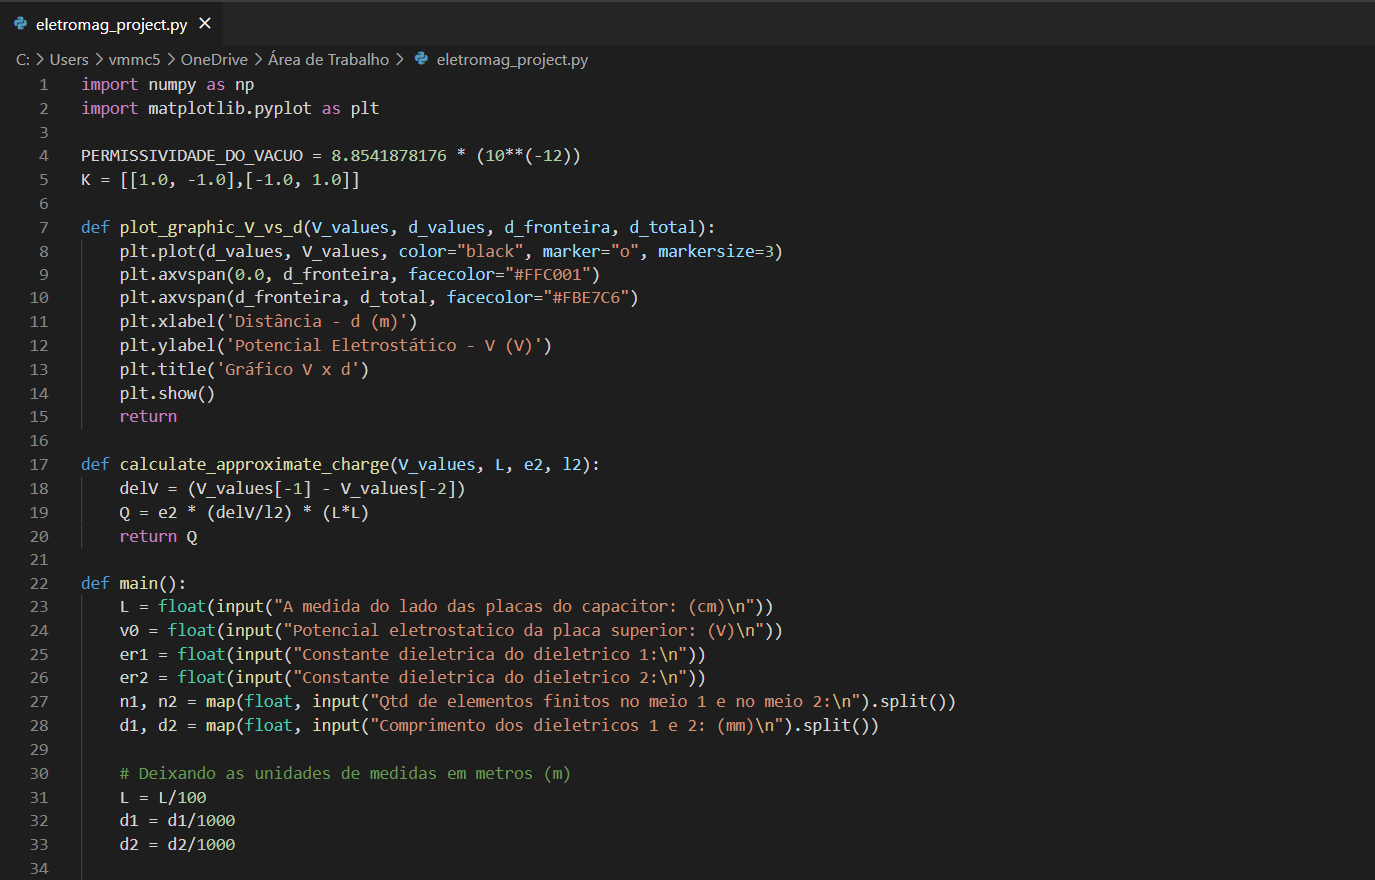
\includegraphics[width=20cm,height=22cm]{CodigoProjeto/eletromag_project_1.png}}
    \caption{Código - Parte 1}
    \label{fig:fp14}
    \end{figure}
    
    \begin{figure}[!htb]
    \centerline{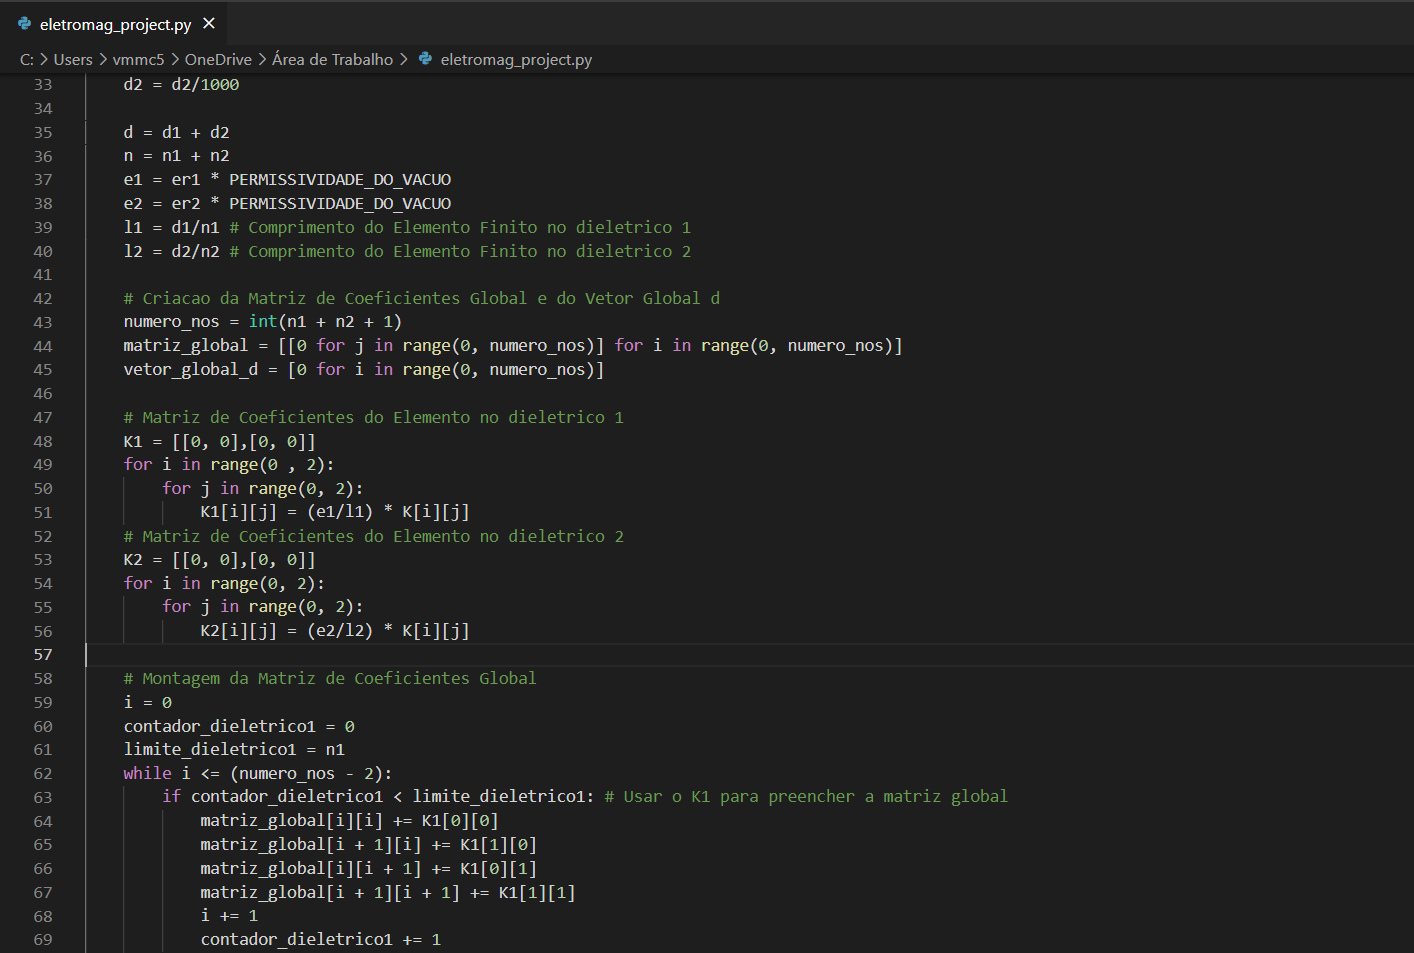
\includegraphics[width=20cm,height=22cm]{CodigoProjeto/eletromag_project_2.png}}
    \caption{Código - Parte 2}
    \label{fig:fp14}
    \end{figure}
    
    \begin{figure}[!htb]
    \centerline{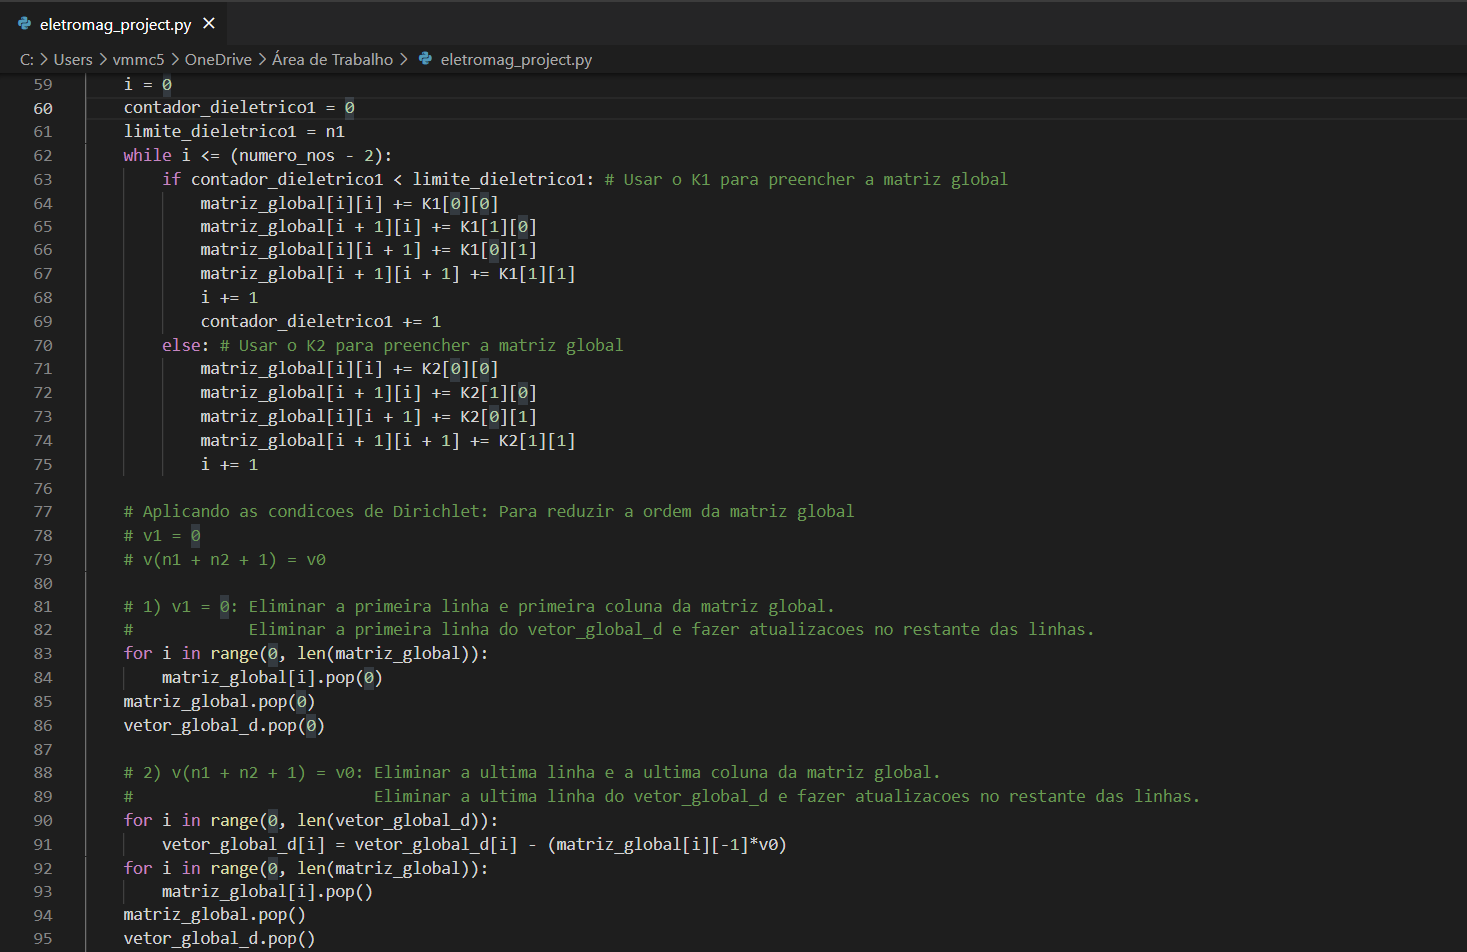
\includegraphics[width=20cm,height=22cm]{CodigoProjeto/eletromag_project_3.png}}
    \caption{Código - Parte 3}
    \label{fig:fp14}
    \end{figure}
    
    \begin{figure}[!htb]
    \centerline{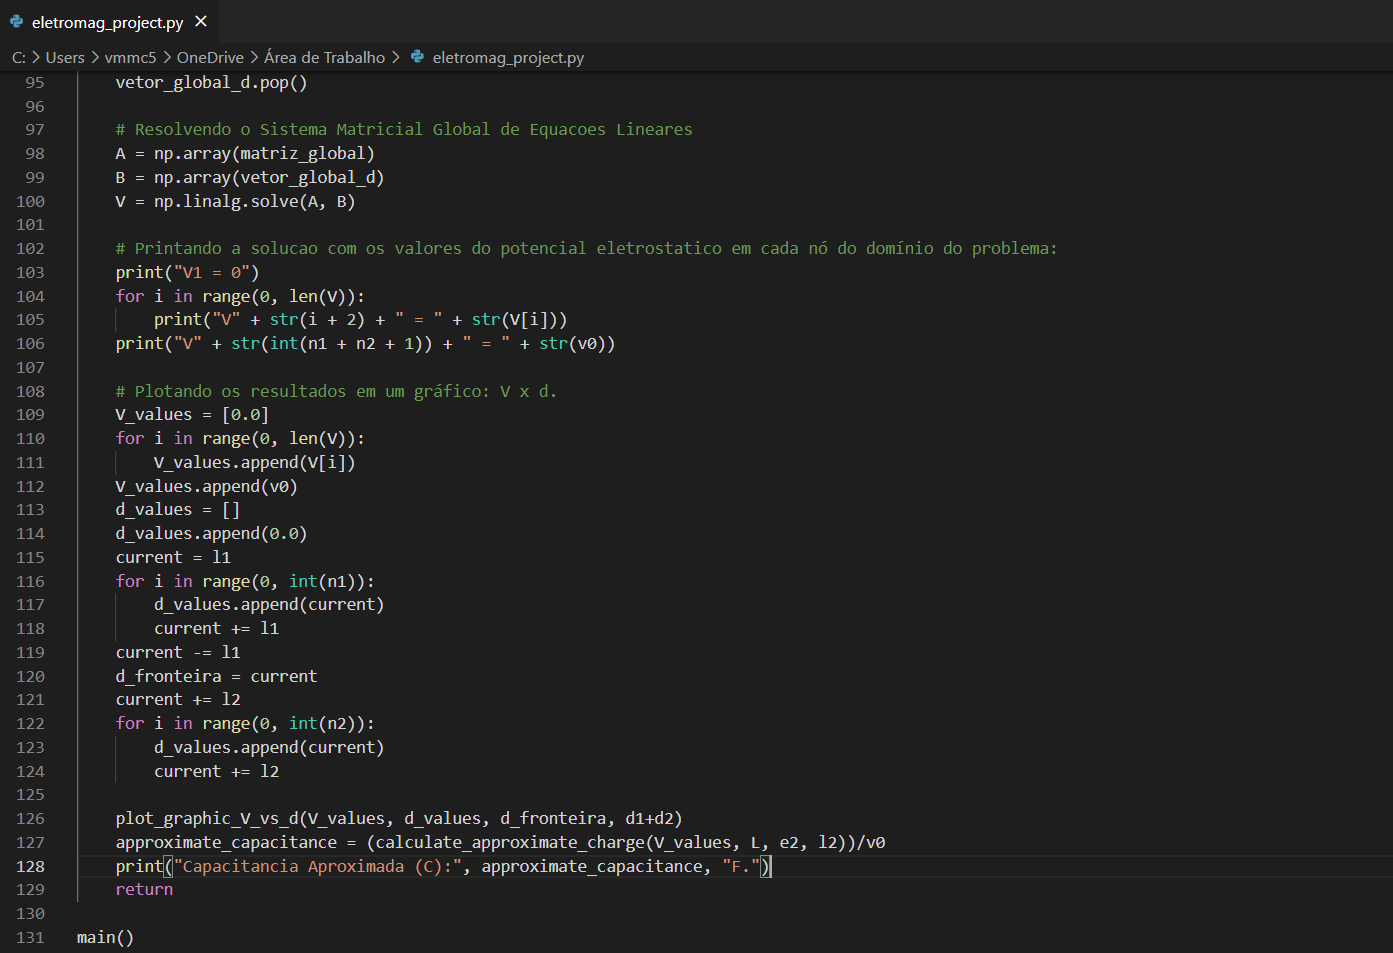
\includegraphics[width=20cm,height=22cm]{CodigoProjeto/eletromag_project_4.png}}
    \caption{Código - Parte 4}
    \label{fig:fp14}
    \end{figure}
    
\section{Obtenção do sistema linear e cálculo do potencial eletrostático aproximado para um caso específico}
    
    \begin{itemize}
    \item Para o caso específico fornecido temos os seguintes dados de antemão:
        \begin{itemize}
        \item $L$ = 2 cm
        \item $d_{1}$ = 1 mm
        \item $d_{2}$ = 1 mm
        \item $\epsilon_{r1}$ = 2
        \item $\epsilon_{r2}$ = 4
        \item $V_{0}$ = 1 V
        \end{itemize}
    \item Os valores de $n_{1}$, $n_{2}$ e $n = n_{1} + n_{2}$ estão livres para serem escolhidos. Logo, por questões de simplicidade:
        \begin{itemize}
        \item $n_{1}$ = 2
        \item $n_{2}$ = 2
        \item $n$ = 4
        \end{itemize}
    \item Segue abaixo a aproximação para o potencial eletrostático entre as placas do capacitor fornecido:
    
    \begin{figure}[!htb]
    \centerline{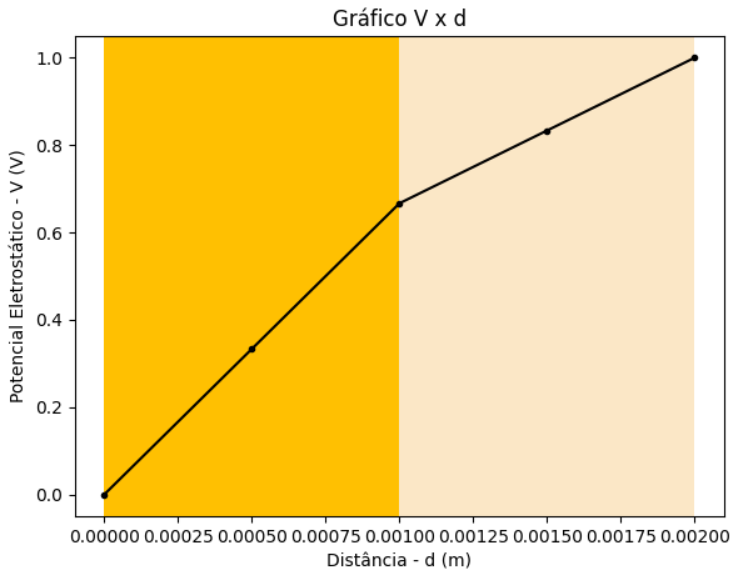
\includegraphics[width=12cm,height=12cm]{Graficos/Plot 1 - 2 2.png}}
    \caption{Gráfico 1 - $n_{1}$ = 2, $n_{2}$ = 2 }
    \label{fig:fp14}
    \end{figure}
    
    \newpage
    \item O potencial em cada um dos $n_{1} + n_{2} + 1$ (5) nós do domínio é dado pela solução do respectivo sistema linear:
        \begin{itemize}
        \item $V_{1}$ = 0 V
        \item $V_{2}$ = 0.3333333 V
        \item $V_{3}$ = 0.6666666 V
        \item $V_{4}$ = 0.8333334 V
        \item $V_{5}$ = 1 V
        \end{itemize}
    \item Segue abaixo a formulação matemática necessária para obter o sistema linear para esse caso específico:
    
    \begin{figure}[!htb]
    \centerline{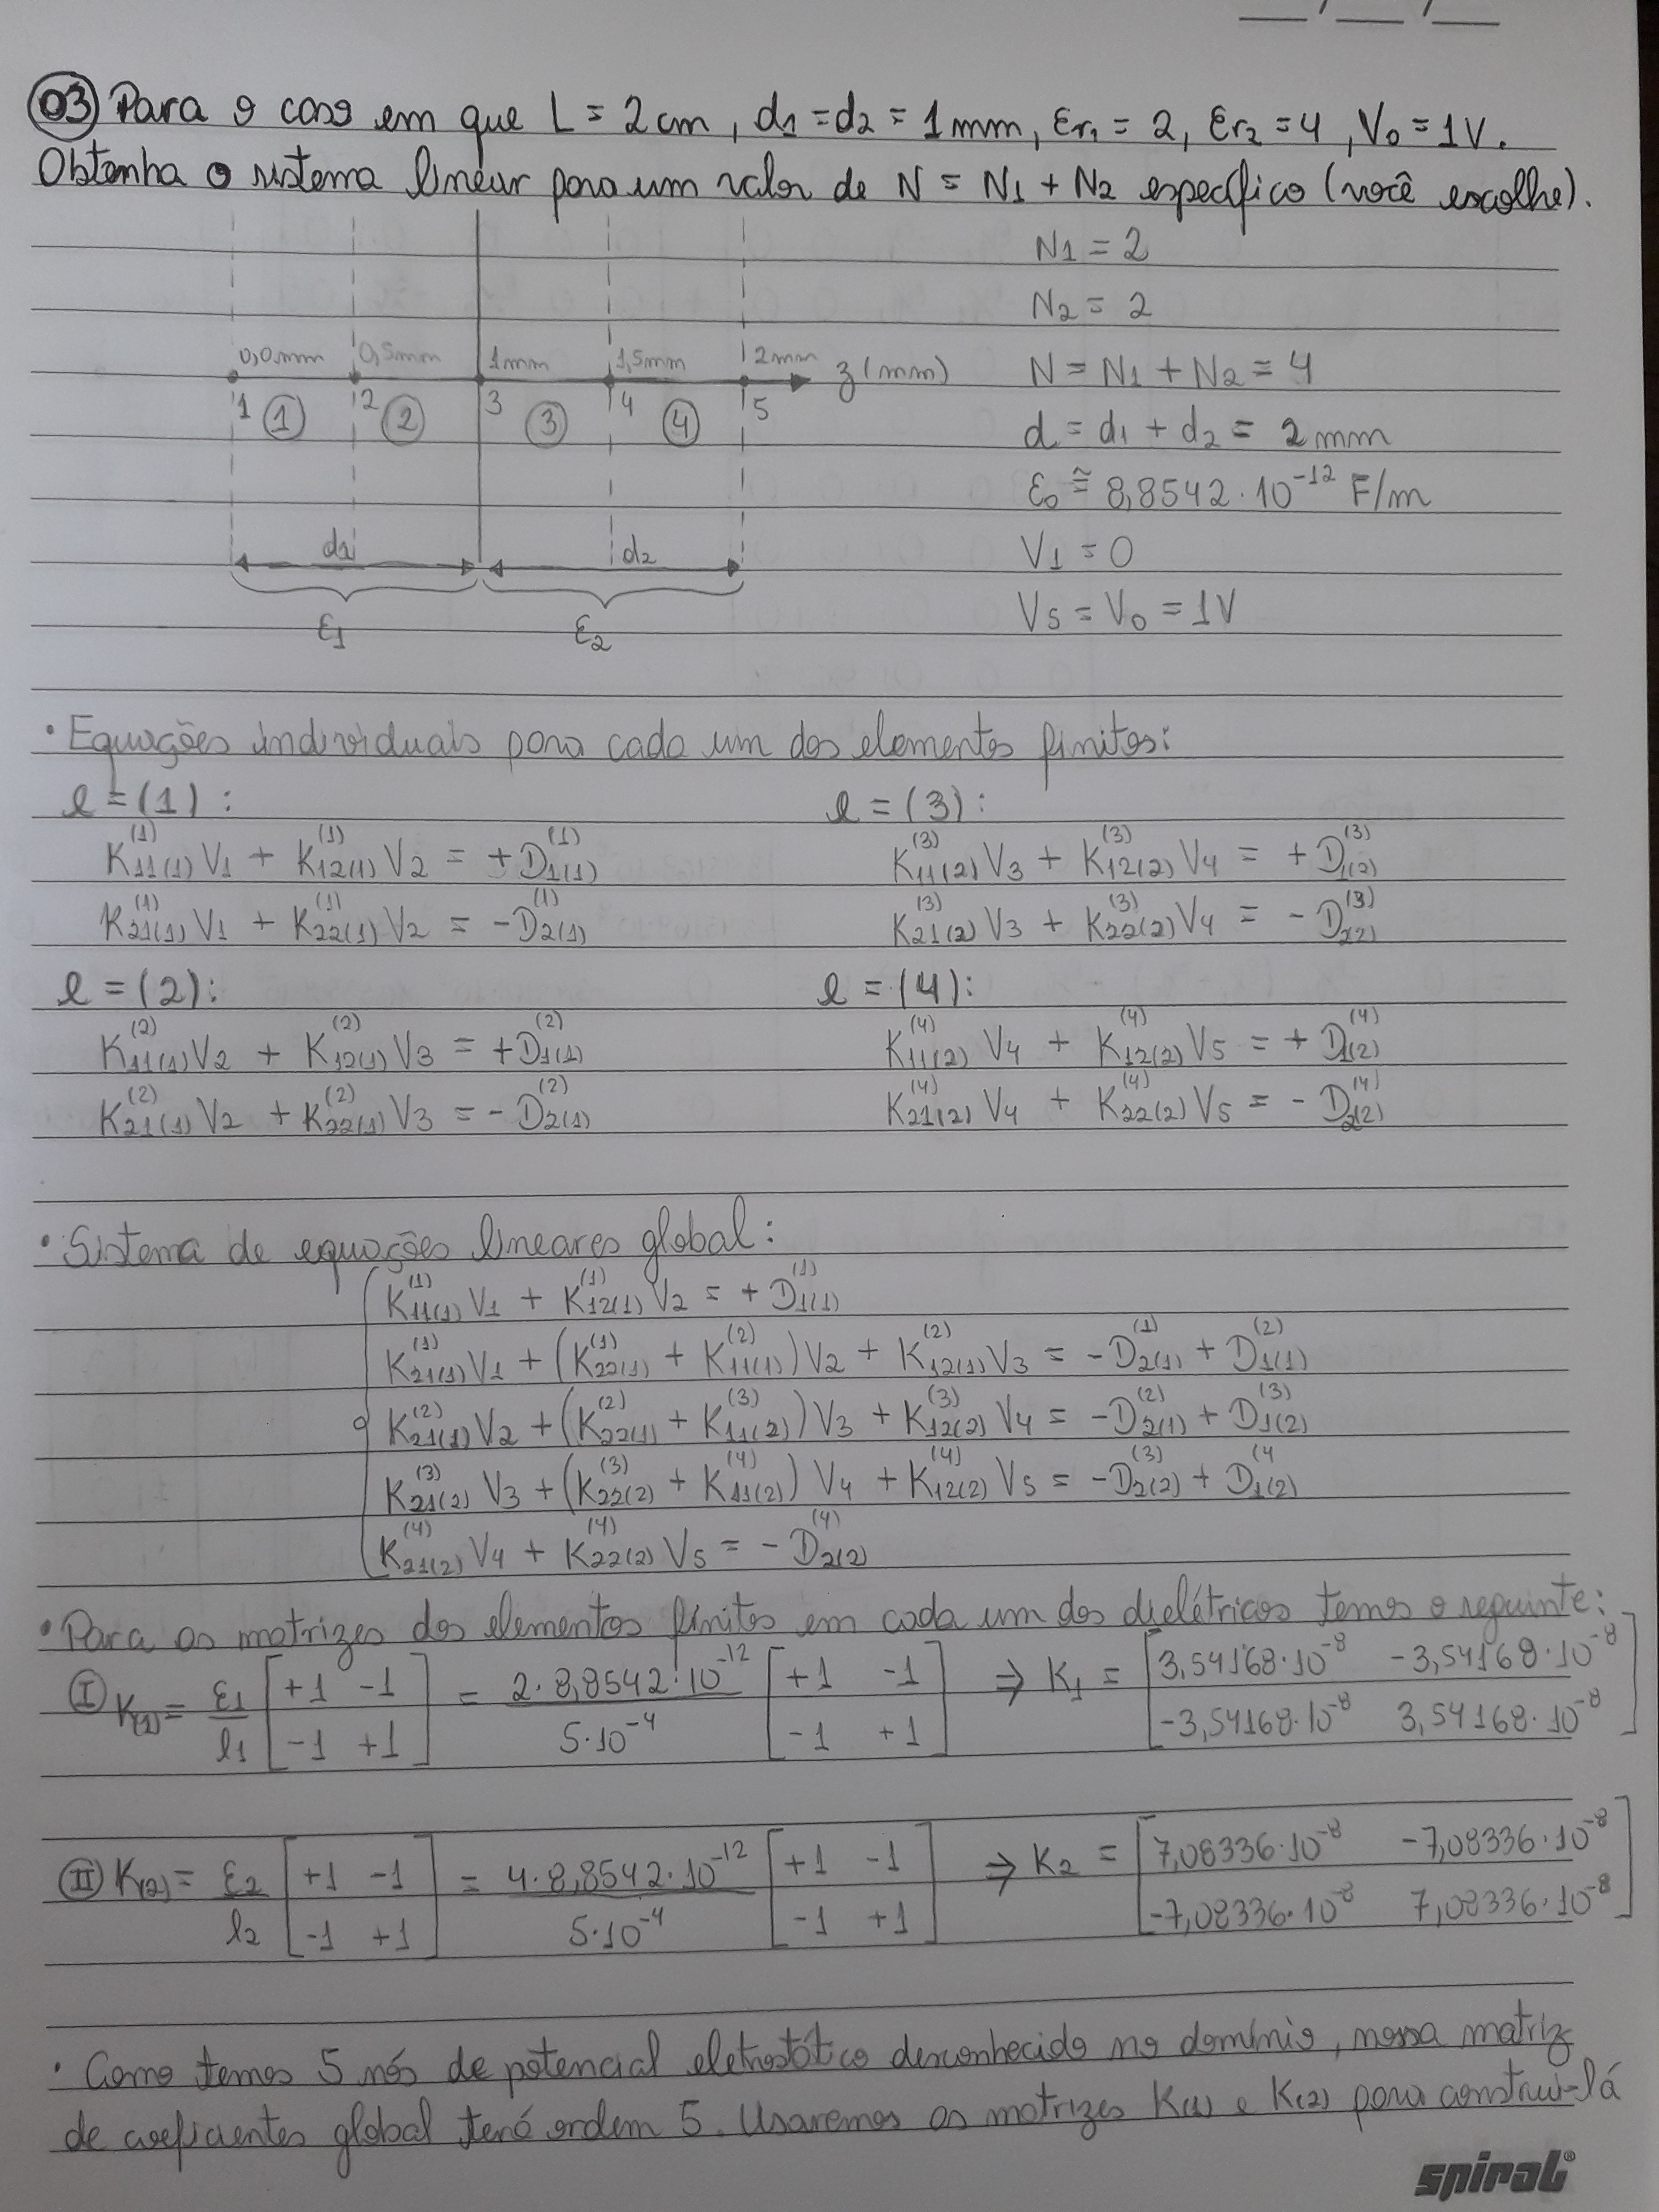
\includegraphics[width=16cm,height=17cm]{FormulaçõesExtras/f1.jpg}}
    \caption{Parte 1}
    \label{fig:f1}
    \end{figure}
    
    \begin{figure}[!htb]
    \centerline{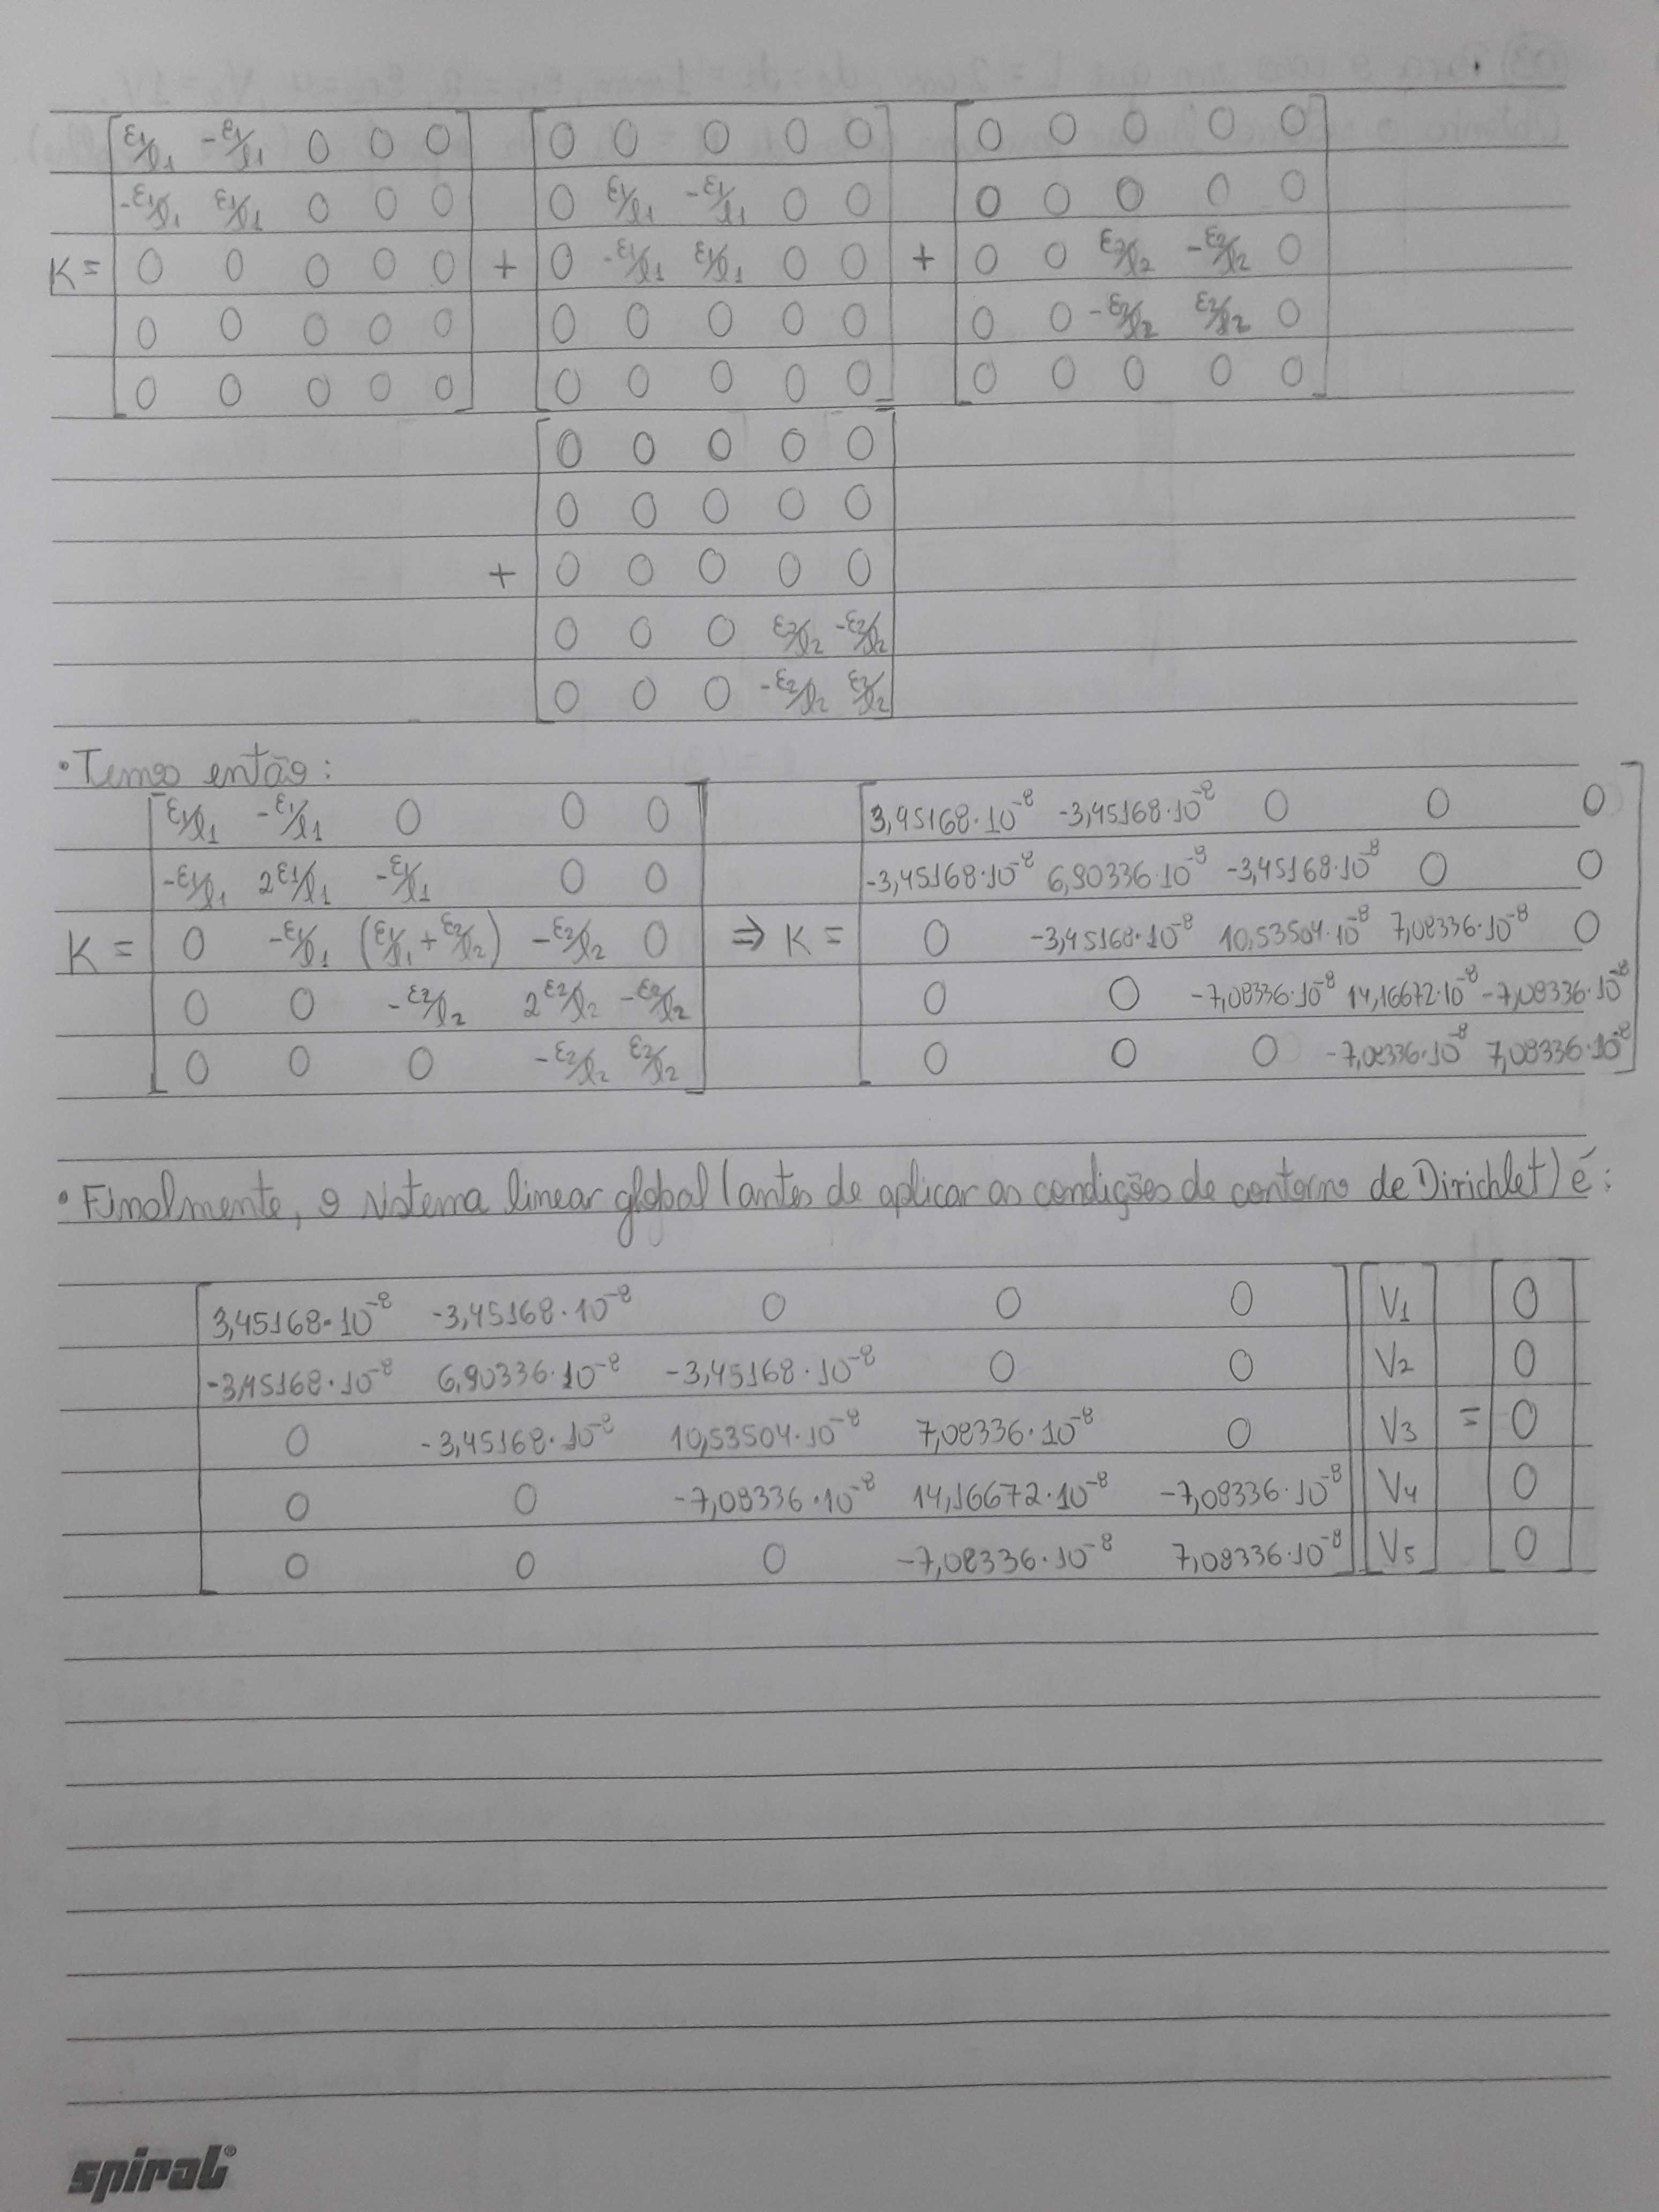
\includegraphics[width=20cm,height=22cm]{FormulaçõesExtras/f2.jpg}}
    \caption{Parte 2}
    \label{fig:f2}
    \end{figure}
    
    \end{itemize}
    
\section{Comparativo entre os valores do potencial eletrostático obtidos para diferentes valores de N}
    
    \begin{itemize}
    \item Gráfico 1: Potencial eletrostático V x Distância d. ($n_{1}$ = 2, $n_{2}$ = 2).
    \begin{figure}[!htb]
    \centerline{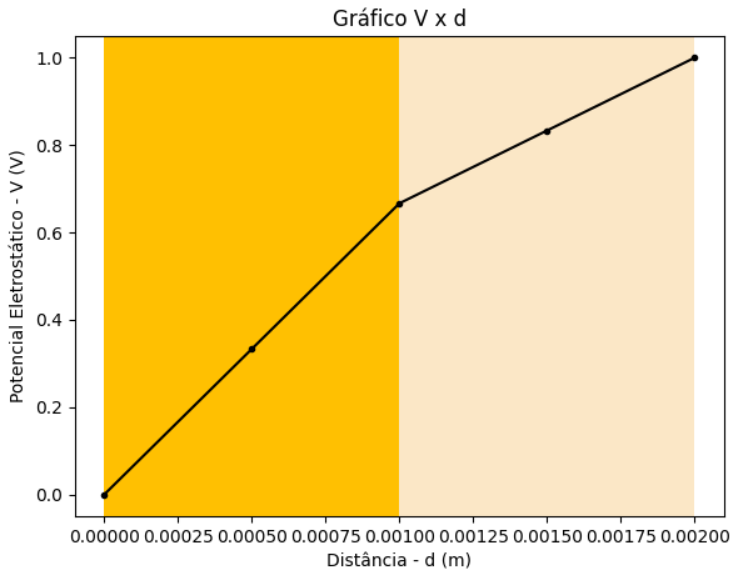
\includegraphics[width=7cm,height=7cm]{Graficos/Plot 1 - 2 2.png}}
    \caption{Gráfico 1}
    \label{fig:f2}
    \end{figure}
    
    \item Gráfico 2: Potencial eletrostático V x Distância d. ($n_{1}$ = 10, $n_{2}$ = 10).
    \begin{figure}[!htb]
    \centerline{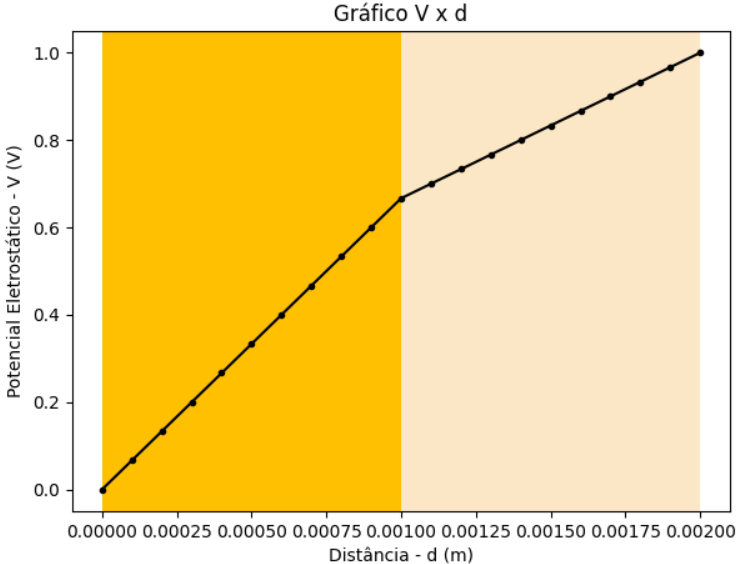
\includegraphics[width=7cm,height=7cm]{Graficos/Plot 2 - 10 10.png}}
    \caption{Gráfico 2}
    \label{fig:f2}
    \end{figure}
    \end{itemize}
    \newpage
    
    \begin{itemize}
    \item Gráfico 3: Potencial eletrostático V x Distância d. ($n_{1}$ = 20, $n_{2}$ = 40).
    \begin{figure}[!htb]
    \centerline{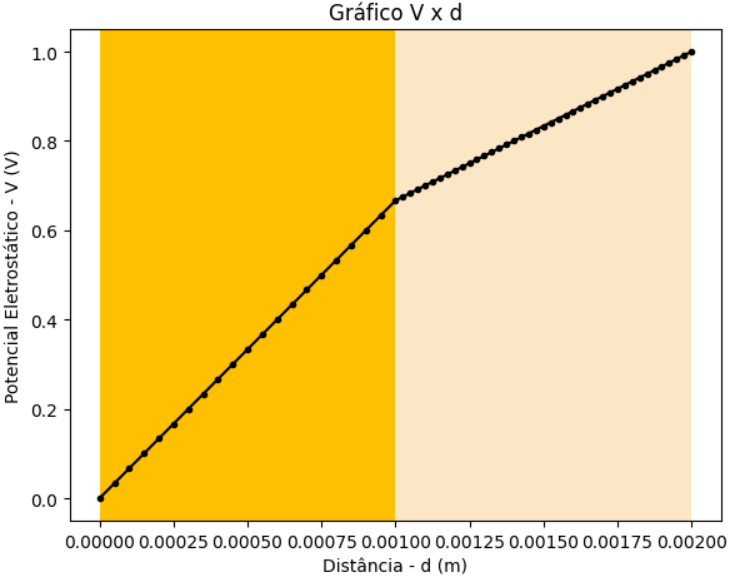
\includegraphics[width=7cm,height=7cm]{Graficos/Plot 3 - 20 40.png}}
    \caption{Gráfico 3}
    \label{fig:f2}
    \end{figure}
    
    \item Gráfico 4: Potencial eletrostático V x Distância d. ($n_{1}$ = 100, $n_{2}$ = 50).
    \begin{figure}[!htb]
    \centerline{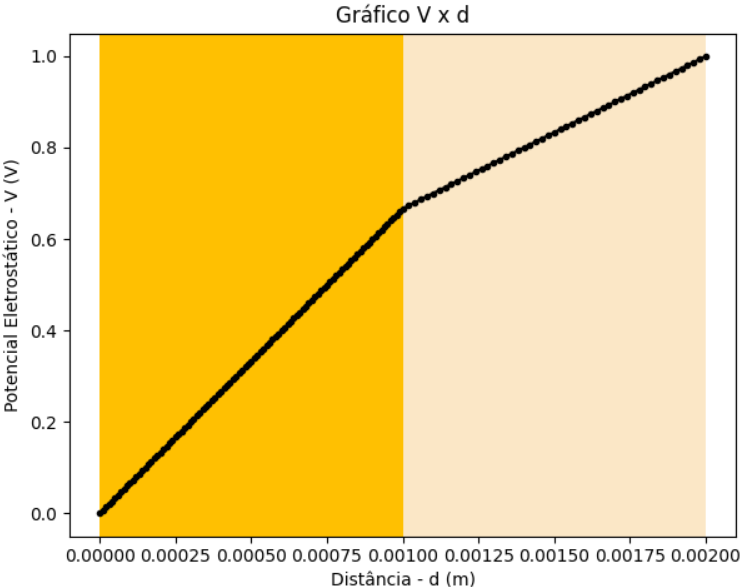
\includegraphics[width=7cm,height=7cm]{Graficos/Plot 4 - 100 50.png}}
    \caption{Gráfico 4}
    \label{fig:f2}
    \end{figure}
    
    \item Analisando os 4 gráficos plotados acima, é perceptível que, para os valores fornecidos no item 3, não há diferenças nos valores dos potenciais eletrostáticos calculados em cada um dos nós.
    \item Isso acontece, pois o fato de não existir cargas livres no interior dos dielétricos implica que a densidade de cargas dentro deles é nula: $\rho = 0$. Logo, ao resolver analiticamente esse problema, temos que a equação de Poisson ($\nabla^{2}V = \frac{-\rho}{\epsilon}$) se torna a equação de Laplace ($\nabla^{2}V = 0$). Consequentemente, a solução , dadas as condições de contorno,  é linear (polinômio de grau 1): $V = ax + b$. O que é exatamente igual ao que foi desenvolvido no método numérico aqui proposto. Como a solução do método teórico/analítico é igual a solução do método numérico, discretizar o domínio em mais elementos finitos não deixará o resultado mais preciso. Novamente, essa equivalência entre aos metados se deve ao fato de que: $\rho = 0$.
    
    \end{itemize}
    \newpage

\section{Comparativo entre os valores da capacitância obtidos para diferentes valores de N e o obtido teoricamente}
    \begin{itemize}
    \item O valor teórico da capacitância $C$ de um capacitor de placas paralelas, que possui 2 dielétricos em série, é dado por:
    
    \begin{figure}[!htb]
    \centerline{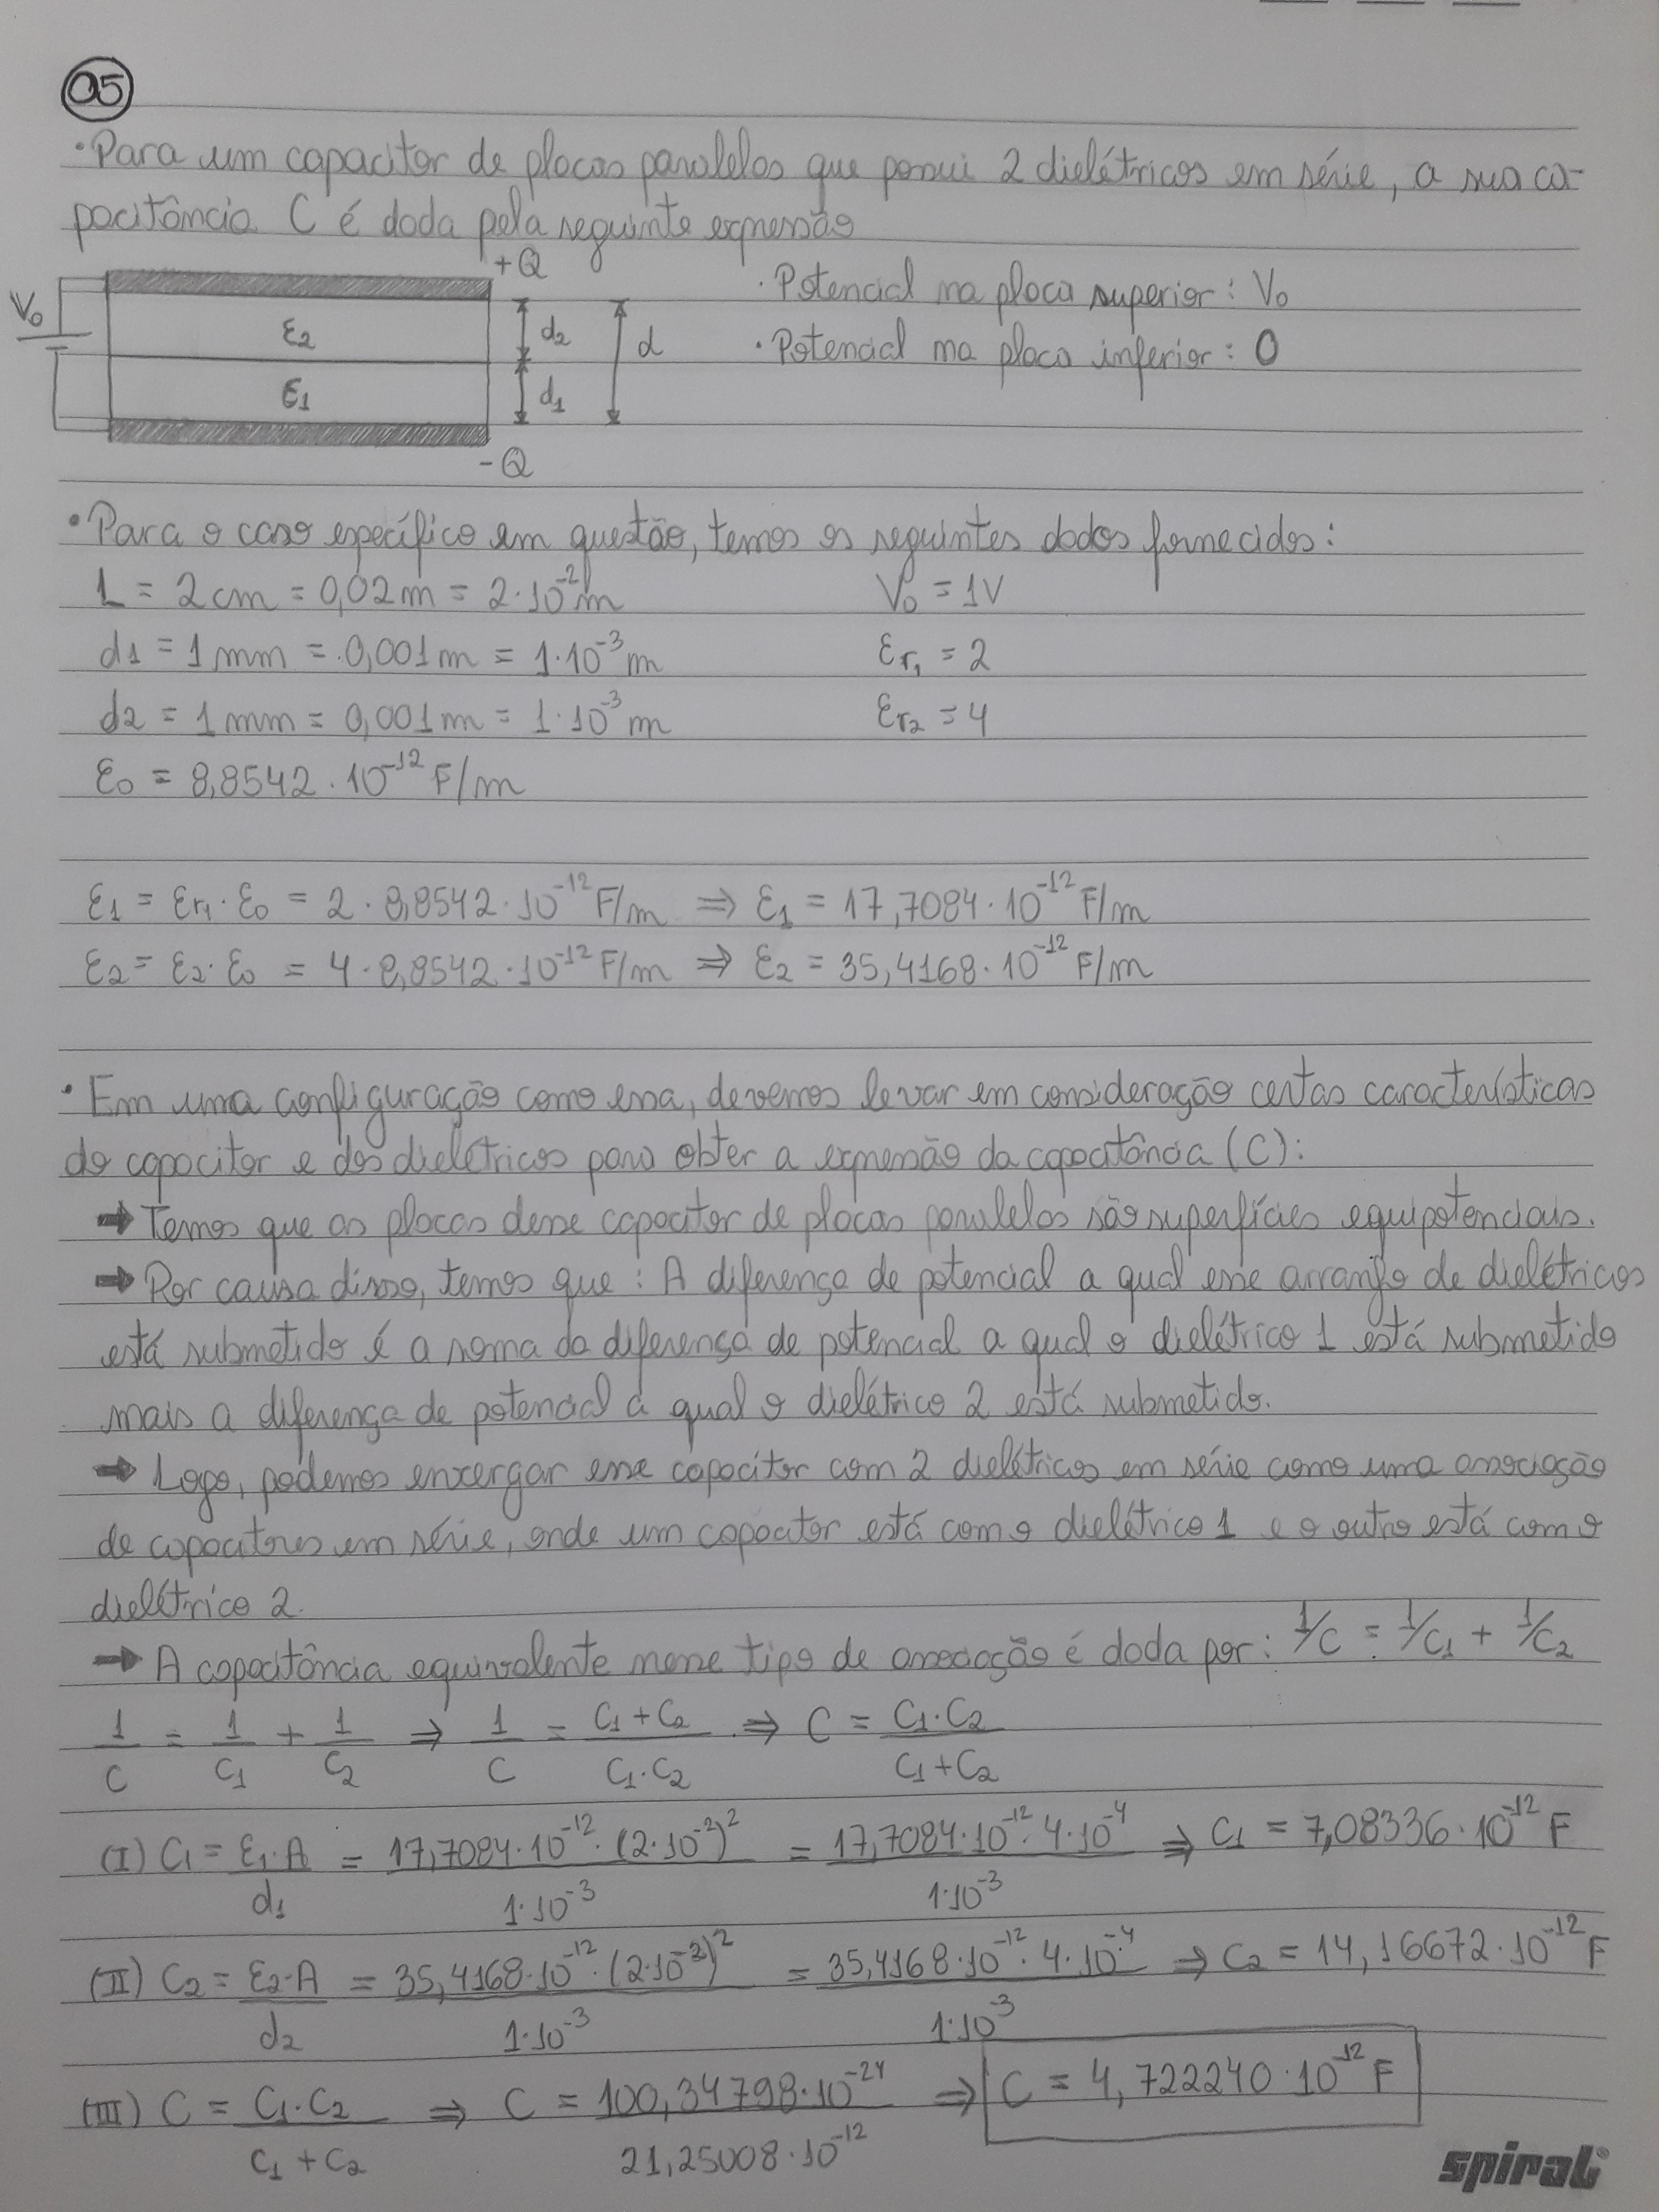
\includegraphics[width=16cm,height=20cm]{capacitancia_teorica.jpg}}
    \caption{Formulação para valor teórico da capacitância $C$}
    \label{fig:f1}
    \end{figure}
    
    \item O valor da capacitância $C$ também pode ser obtido pelo método numérico dos elementos finitos aqui apresentado.
    \item Para isso, a definição da capacitância $C$ diz que: $C = \frac{Q}{V}$. O valor de $V$ é dado pela diferença entre o potencial eletrostático no último nó e  potencial eletrostático no primeiro nó do domínio discretizado. Já a carga $Q$ pode ser estimada.
    \item Para estimar a carga $Q$ será calculada a densidade superficial de carga $\sigma$ na placa superior do capacitor e, usando as dimensões da placa fornecidas no enunciado, a carga poderá ser calculada.
    \item Para a situação do capacitor de placas paralelas que possui um dielétrico entre elas, a condição de contorno da eletrostática é: $\sigma = -\epsilon_{2}\frac{\partial V}{\partial n}$. Onde $n$ é o vetor unitário perpendicular a placa superior do capacitor. Sabendo que $\hat{z} = -n$, a expressão anterior se torna: $\sigma = \epsilon_{2}\frac{\partial V}{\partial z}$
    \item Lembrando que: $Q = \sigma A = \sigma L^{2}$.
    \item Além disso, a expressão $\frac{\partial V}{\partial z}$ pode ser substituída pela aproximação: $\frac{V_{n_{1} + n{2} + 1} - V_{n_{1} + n_{2}}}{l_{2}}$, onde o numerador é a diferença de potencial eletrostático entre os dois últimos nós do domínio e o denominador é o comprimento de um elemento finito no dielétrico 2. Essa aproximação se torna melhor quanto mais elementos são utilizados para discretizar o domínio.
    \item Substituindo essas expressões na expressão inicial da capacitância ($C = \frac{Q}{V}$), têm-se o seguinte: $C = \epsilon_{2}\frac{(\frac{V_{n_{1} + n_{2} + 1} - V_{n_{1} + n_{2}}}{l_{2}})}{V_{n_{1} + n_{2} + 1} - V_{1}}L^{2}$.
    \item Fazendo o comparativo do valor da capacitância $C$ calculado para 6 valores diferentes de $n_{1}$ e $n_{2}$:
    \begin{itemize}
        \item Para $n_{1}$ = 2 e $n_{2}$ = 2, têm-se: $C$ = 4.722233502719999 \cdot $10^{-12}$ F.
        \item Para $n_{1}$ = 50 e $n_{2}$ = 50, têm-se: $C$ = 4.722233502720502 \cdot $10^{-12}$ F.
        \item Para $n_{1}$ = 80 e $n_{2}$ = 60, têm-se: $C$ = 4.722233502720549 \cdot $10^{-12}$ F.
        \item Para $n_{1}$ = 100 e $n_{2}$ = 120, têm-se: $C$ = 4.722233502722625 \cdot $10^{-12}$ F.
        \item Para $n_{1}$ = 2000 e $n_{2}$ = 2000, têm-se: $C$ = 4.722233502744645 \cdot $10^{-12}$ F.
        \item Para $n_{1}$ = 5000 e $n_{2}$ = 5000, têm-se: $C$ = 4.722233502798121 \cdot $10^{-12}$ F.
    \end{itemize}
    \item Conclui-se que o valor da capacitância $C$ calculado pelo método dos elementos finitos tende lentamente ao valor teórico da capacitância (a medida que se aumenta os valores de $n_{1}$ e $n_{2}$), conforme esperado.
    
    
    \end{itemize}

\section{Referências}
    \begin{itemize}
    \item Elementos de Eletromagnetismo, Matthew Sadiku, 3 Ed., 2006.
    \item Introduction to Electrodynamics, David Griffiths, 3 Ed., 1999.
    \item Introduction to the Finite Element Method in Electromagnetics, Anastasis C. Polycarpou, 2006.
    \end{itemize}
    
\end{document}